%
% Physical Architectures For Quantum Computing
%

\section{Physical architectures for quantum computing} \label{sec:archs_QC} \index{Physical architectures}

\dropcap{T}{he} models for quantum computation introduced in the previous section are abstractions of algorithms in terms of elementary operations. But elementary operations must ultimately be physically realised. There are countless physical architectures for realising quantum computations, far too many to describe here, each with their own advantages and disadvantages, and it is far from clear which physical architecture(s) will ultimately win the quantum race.

Here we will summarise some of the physical architectures most applicable to networking. Since we reasonably anticipate that future quantum networking will be optically mediated, we focus on pure-optical and hybrid-optical architectures, on the basis that these will naturally lend themselves to optical interfacing.

%
% Universal Linear Optics
%

\subsection{Universal linear optics} \label{sec:KLM_univ} \index{Universal linear optics quantum computation}\index{Knill-Laflamme-Milburn (KLM)}

With single-photon encoding of qubits in the quantum network, the obvious architecture to implement quantum computation is linear optics quantum computing (LOQC) \cite{bib:KLM01} (KLM), since the states being processed by the computer are of the same form as the states traversing the network. See \cite{bib:Kok05, bib:KokLovettBook} for excellent introductions to this what has become a very broad and exciting field.

LOQC allows universal quantum computing to be implemented using single-photon polarisation or dual-rail encoding, with only linear optics interactions, i.e beamsplitter/phase-shifter networks \cite{bib:Reck94}, with the addition of quantum memory, and fast-feedforward, whereby some photons are measured, and the remaining part of the optical circuit is dynamically reconfigured based on the measurement outcomes. The former is readily available technology today, and elementary demonstrations have been performed \cite{bib:OBrien03, bib:carolan2015universal}, but the latter two have proven to be somewhat more challenging.

Originally it was believed that universal optical quantum computation, specifically the implementation of 2-qubit entangling gates (such as CNOT or CZ gates), would require extremely (and unrealistically) strong optical non-linearities that implement a non-linear sign-shift (NS) gate,
\begin{align} \label{eq:NS_trans}\index{Non-linear sign-shift (NS) gate}
NS: \alpha\ket{0}+\beta\ket{1}+\gamma\ket{2}\to\alpha\ket{0}+\beta\ket{1}-\gamma\ket{2},
\end{align}
in the photon-number basis, up to normalisation (which is determined by the post-selection success probability). That is, it applies a $\pi$ phase-shift to only the $\ket{2}$ component of a photon-number superposition. The breakthrough result by KLM demonstrated that this is in fact not the case at all. Instead, the NS gate can be implemented non-deterministically using post-selected linear optics. Two such NS gates allow the construction of a single CZ gate. The construction of the KLM NS and CZ gates are shown in Figs.~\ref{fig:KLM_gate} \& \ref{fig:KLM_explain}. Equivalently, a CNOT gate may be trivially constructed via conjugation by Hadamard gates, based on the identity \mbox{$\hat{H}\hat{Z}\hat{H}=\hat{X}$}.

\begin{figure}[!htbp]
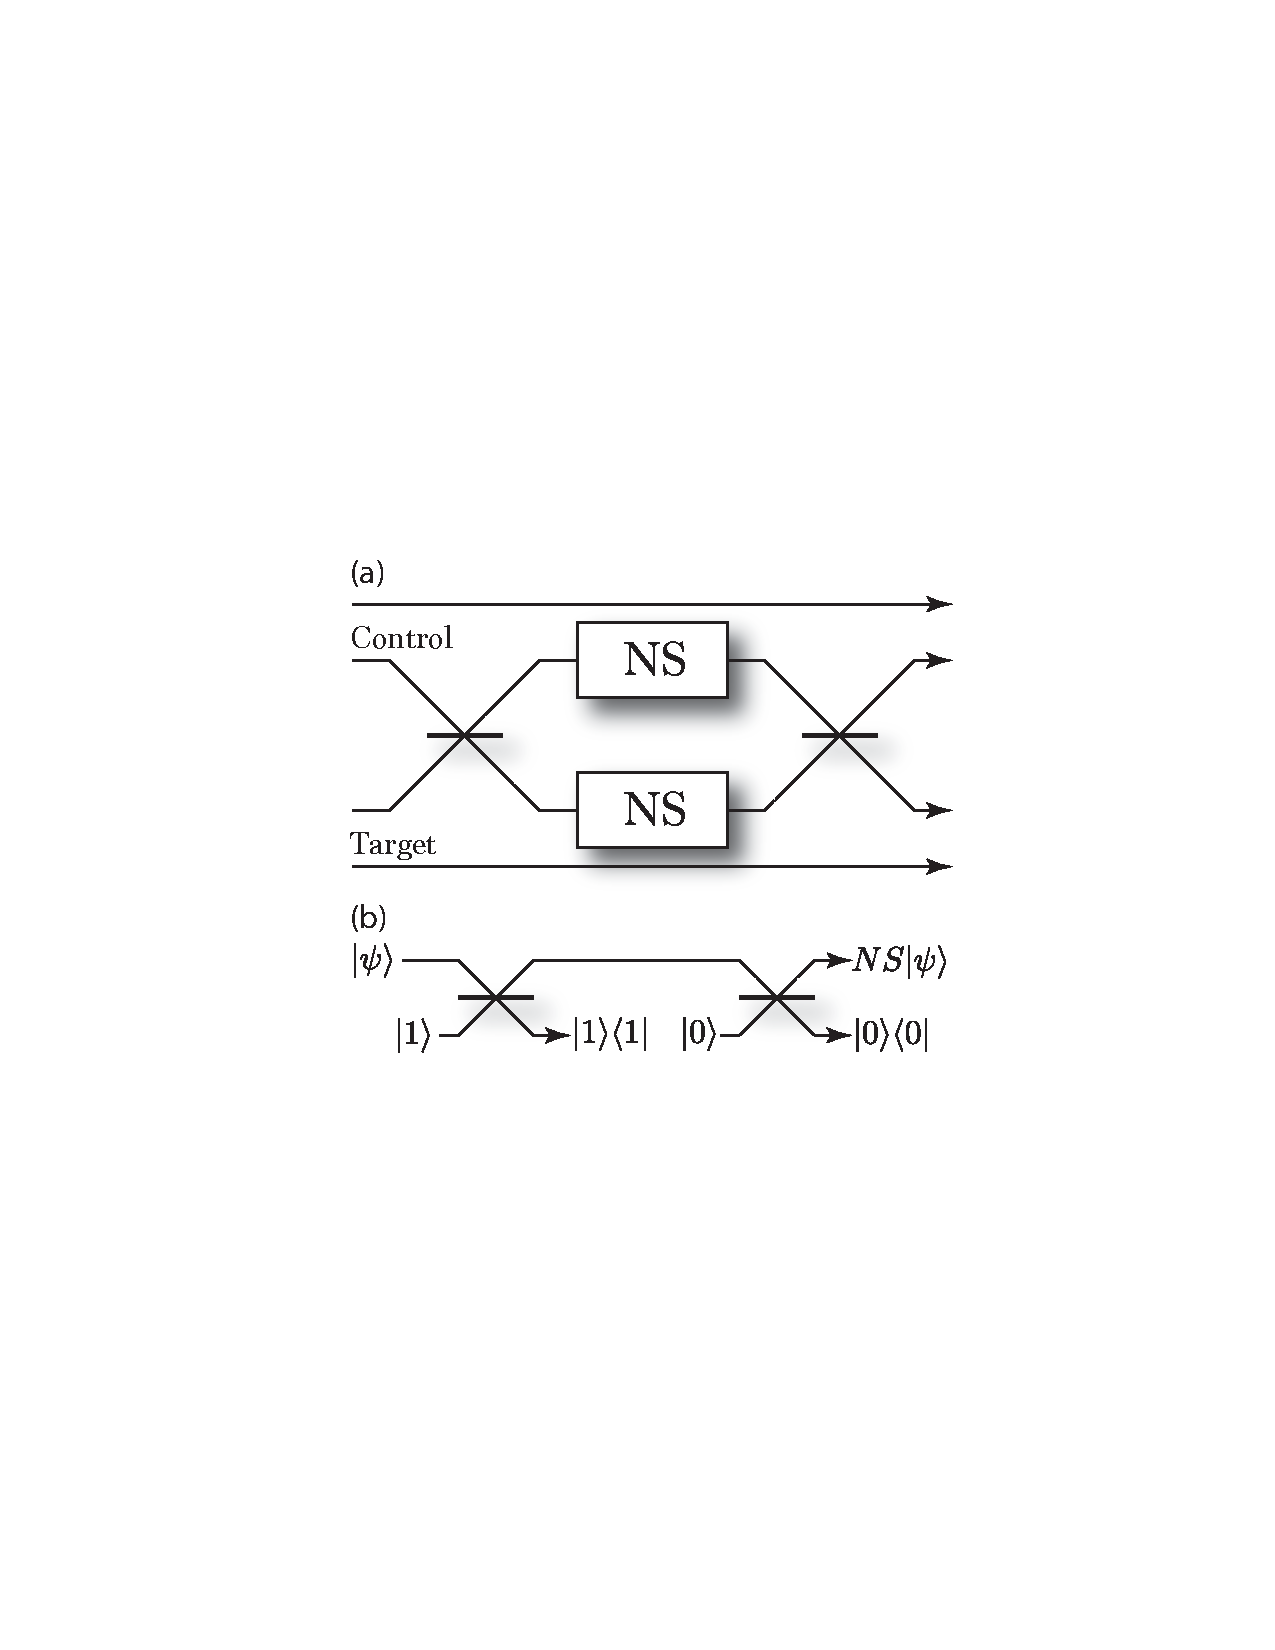
\includegraphics[clip=true, width=0.42\textwidth]{KLM_gate}
\captionspacefig \caption{(a) A KLM CZ gate, employing dual-rail encoding, constructed from two non-linear sign-shift (NS) gates, which apply a $\pi$ phase-shift to only $\ket{2}$ terms in the photon-number basis. (b) Construction of the non-deterministic linear optics NS gate. Two ancillary states -- one $\ket{1}$ and one $\ket{0}$ -- are employed, and two photo-detectors post-select upon detecting $\ket{1}\bra{1}$ and $\ket{0}\bra{0}$ respectively. The beamsplitter reflectivities in (a) are 50:50, and in (b) chosen such that the amplitudes obey Eq.~(\ref{eq:NS_trans}).}. \label{fig:KLM_gate} \index{Knill-Laflamme-Milburn (KLM)}\index{Non-linear sign-shift (NS) gate}
\end{figure}

\if 2\pubmode
	\begin{figure}[!htbp]
	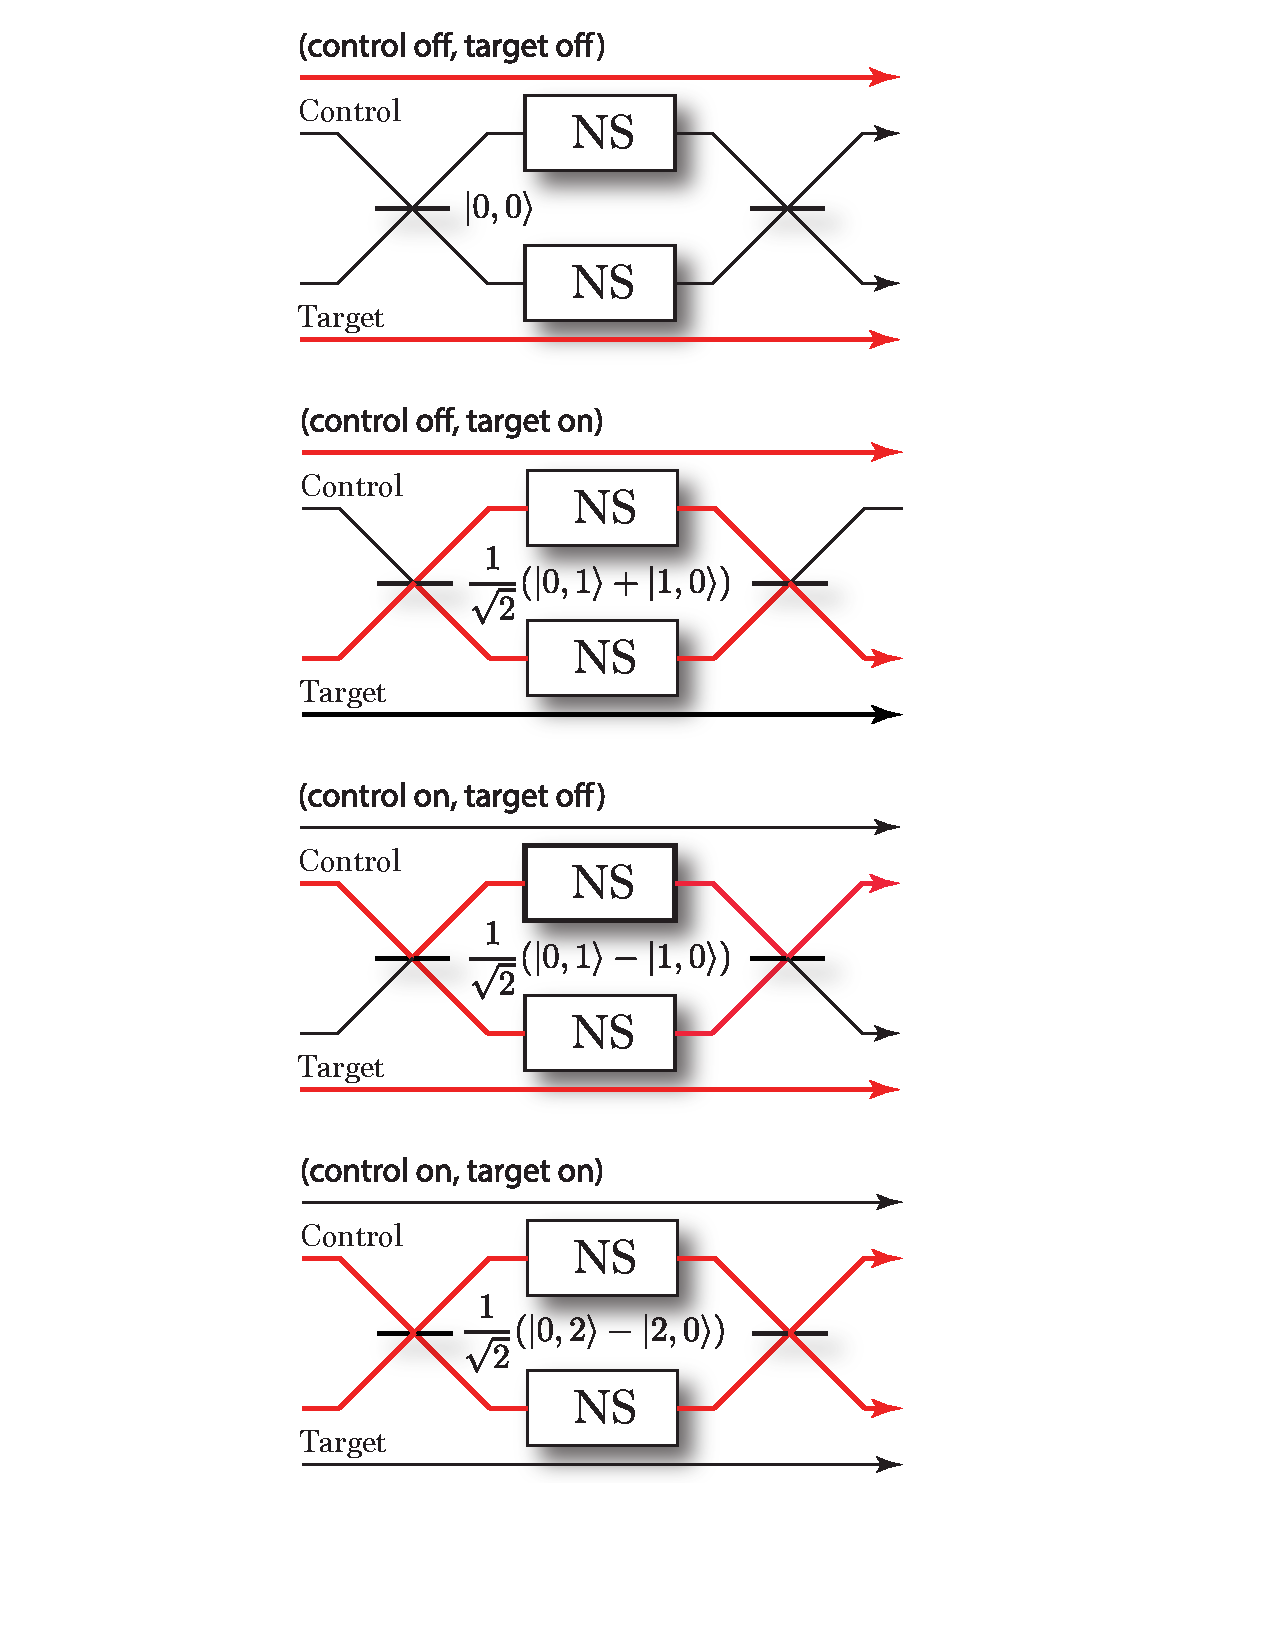
\includegraphics[clip=true, width=0.43\textwidth]{KLM_optical_paths_long}
	\captionspacefig \caption{Evolution of the four logical basis states through the KLM CZ gate. The NS gates do nothing in the first three cases, since they are operating only on vacuum and single-photon terms, which are left unchanged by the NS gate. In the last case, where both control and target are on, HOM interference results in photon bunching after the first beamsplitter, thereby creating two-photon terms. These terms inherit the $\pi$ phase-shift from the NS gate transformation, after which the final beamsplitter reverses the HOM photon bunching, yielding the same logical basis state with an acquired $\pi$ phase-shift.} \label{fig:KLM_explain} \index{Knill-Laflamme-Milburn (KLM)}\index{Controlled-Z (CZ) gates}
	\end{figure}
\else
	\begin{figure*}[!htbp]
	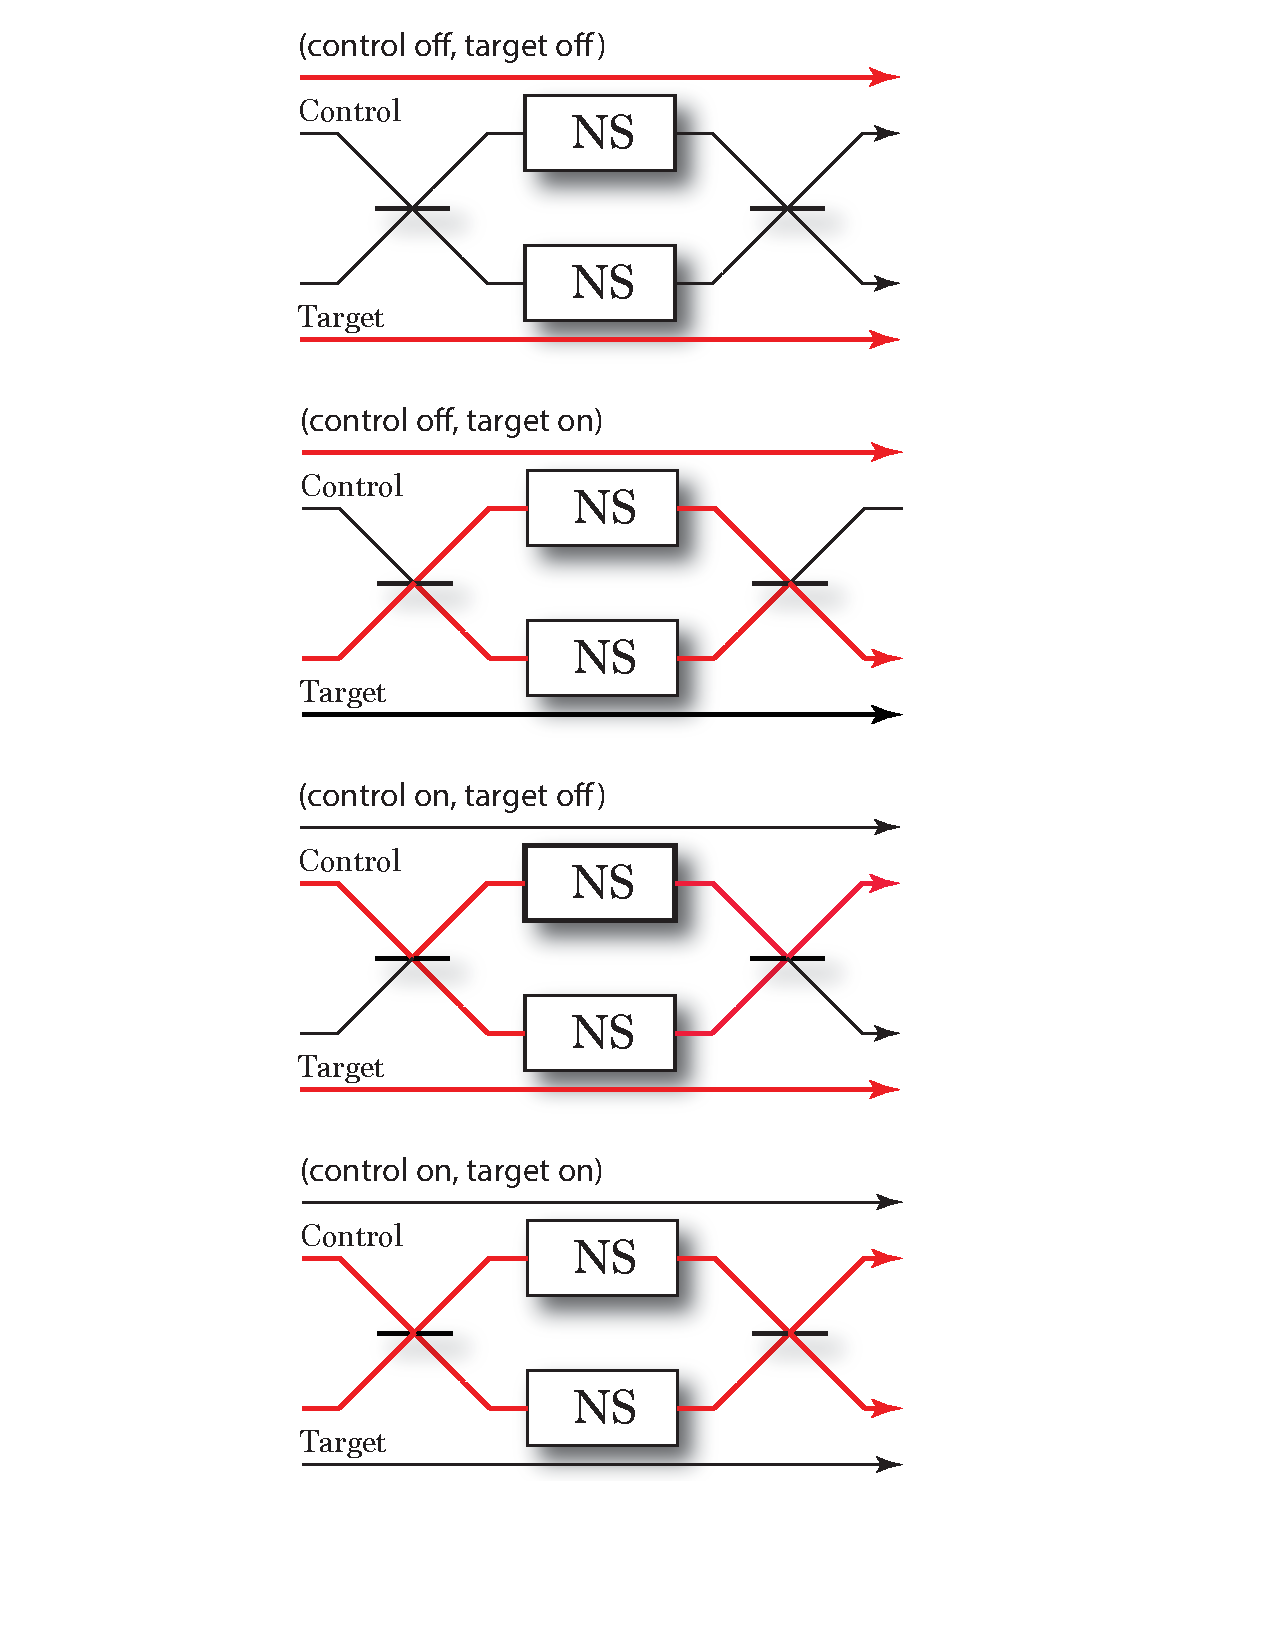
\includegraphics[clip=true, width=0.9\textwidth]{KLM_optical_paths}
	\captionspacefig \caption{Evolution of the four logical basis states through the KLM CZ gate. The NS gates do nothing in the first three cases, since they are operating only on vacuum and single-photon terms, which are left unchanged by the NS gate. In the last case, where both control and target are on, HOM interference results in photon bunching after the first beamsplitter, thereby creating two-photon terms. These terms inherit the $\pi$ phase-shift from the NS gate transformation, after which the final beamsplitter reverses the HOM photon bunching, yielding the same logical basis state with an acquired $\pi$ phase-shift.} \label{fig:KLM_explain} \index{Knill-Laflamme-Milburn (KLM)}\index{Controlled-Z (CZ) gates}
	\end{figure*}
\fi

Clearly this non-determinism is of immediate concern, since concatenating multiple gates would have exponentially decreasing success probability, making the protocol inefficient -- if the probability of a single gate succeeding is $p$, and we require that a circuit comprising $n$ of them all succeed, the success probability is clearly $p^n$.

The first key observation then is that gate teleportation can be used to shift this non-determinism to a resource state preparation stage, as described in detail in Sec.~\ref{sec:teleport_gate}. However, this is not the end of the story, since gate teleportation requires Bell state projections, which are themselves non-deterministic using purely linear optics (either using PBSs or CNOT gates). \latinquote{Ignotum per ignotius}.

The final insight provided by KLM is that by concatenating these non-deterministic CNOT gates, we can inductively build up higher-level CNOT gates with ever increasing success probabilities, asymptoting to unity with high- (but polynomial-) depth concatenation. By combining these key insights, KLM were able to show that near-deterministic CNOT gates can be constructed using an efficient (polynomial) resource overhead, thereby enabling efficient universal quantum computation\footnote{Note that all single-qubit gates are trivially and deterministically implemented using wave-plates or beamsplitters, for polarisation or dual-rail encoding respectively. Thus, we need only concern ourselves with the challenges associated with implementing 2-qubit entangling gates.}. A sketch of the general KLM formalism is shown in Fig.~\ref{fig:KLM_protocol}.

\begin{figure}[!htbp]
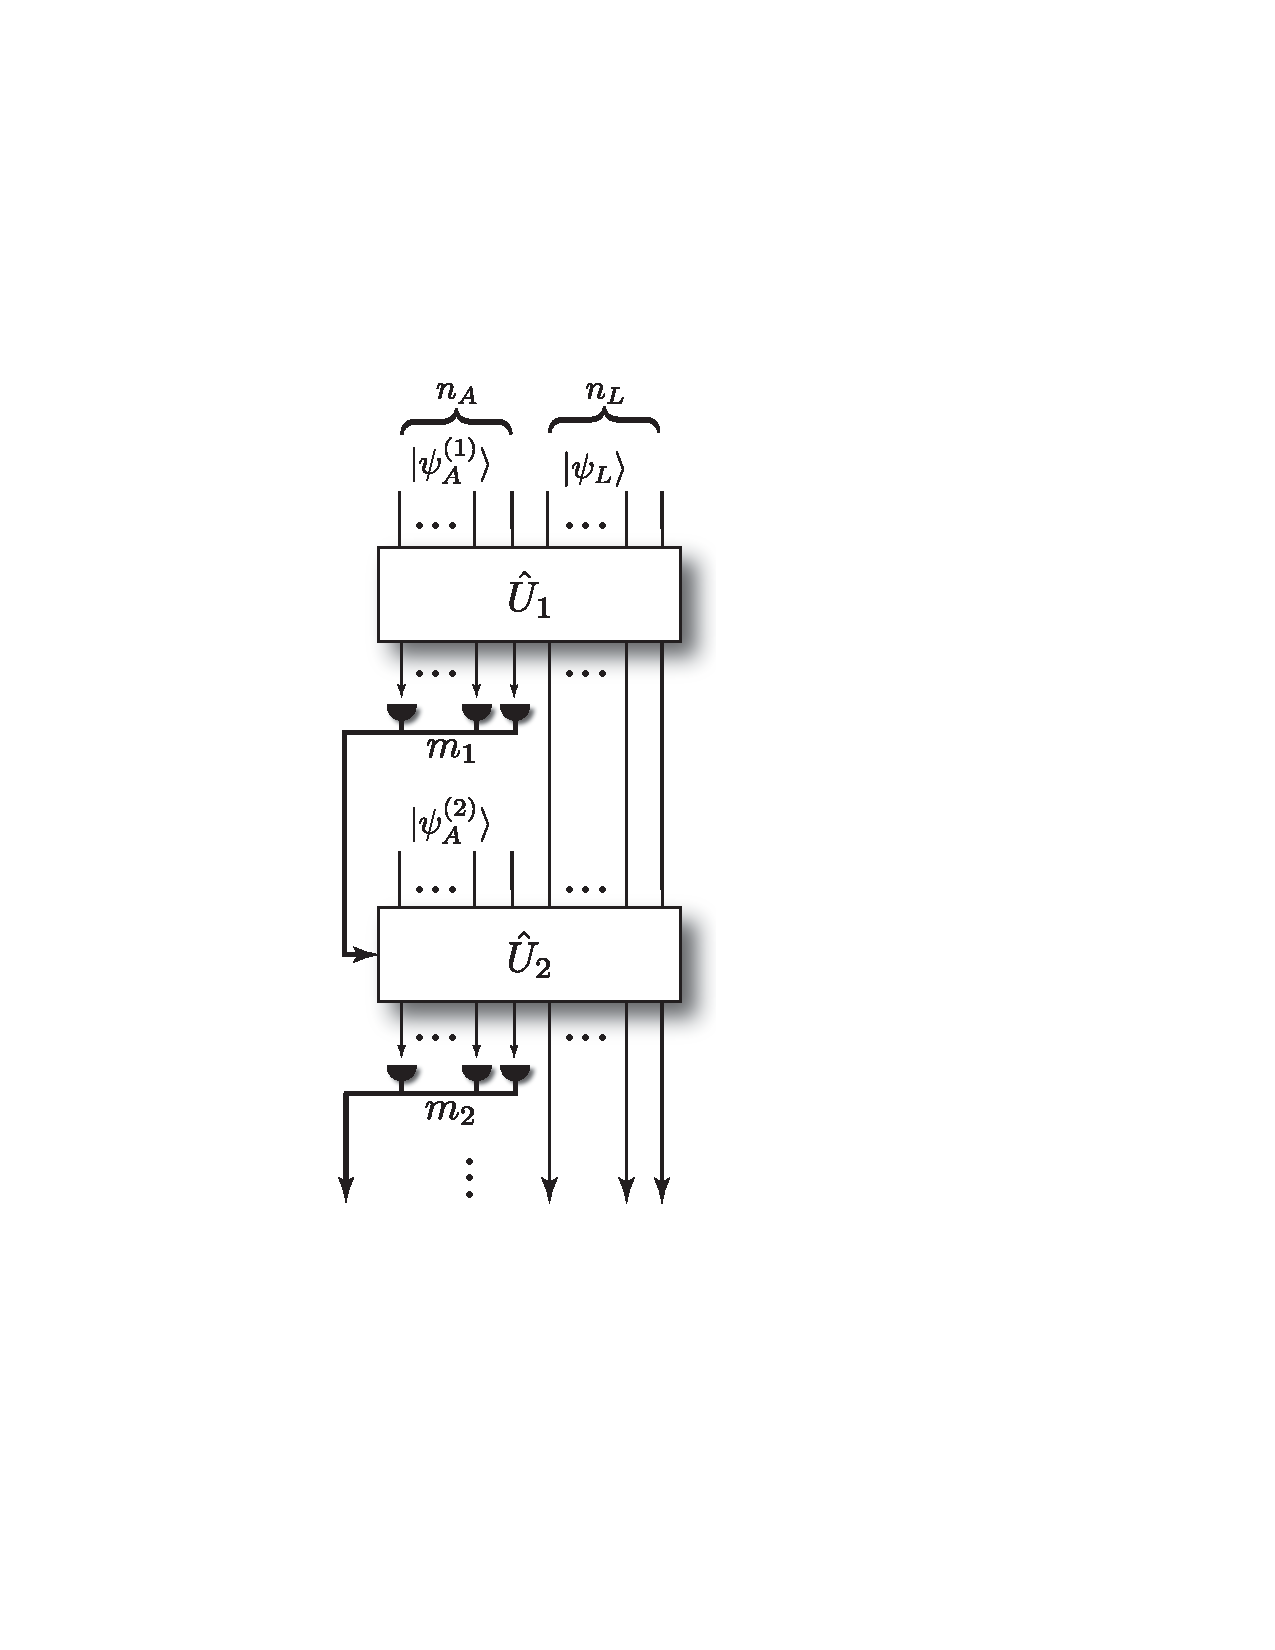
\includegraphics[clip=true, width=0.28\textwidth]{KLM}
\captionspacefig \caption{KLM architecture for universal LOQC. $n_L$ optical modes are associated with logical qubits in the state $\ket{\psi_L}$, with the remaining $n_A$ modes acting as ancillary states, $\ket{\psi_A}$. A round of passive linear optics is applied, $\hat{U}_1$. Then the ancillary modes are measured, yielding some set of measurement outcomes $m_1$. These are classically processed to determine what the next round of passive linear optics, $\hat{U}_2$, ought to be. This repeats some polynomial number of times, from which an arbitrary quantum computation can be implemented. The \textsc{BosonSampling} and quantum walk models are equivalent to taking just the first stage of this protocol: one round of input state, passive linear optics, and measurement.} \label{fig:KLM_protocol}\index{Knill-Laflamme-Milburn (KLM)}
\end{figure}

Evolution via linear optics implements transformations of the form of Eq.~(\ref{eq:LO_unitary_map}), and may be implemented using the experimental architectures described in Sec.~\ref{sec:LO_ev_archs} and Fig.~\ref{fig:LO_archs}.

The measurements are implemented simply by number-resolved photo-detectors, implementing measurement projectors of the form \mbox{$\hat\Pi_n=\ket{n}\bra{n}$}, for the measurement outcome of $n$ photons (Sec.~\ref{sec:photo_detection}).

Since the original presentation of a universal LOQC gate set by KLM, numerous alternate implementations have been presented and experimentally demonstrated, with various pros and cons \cite{bib:Ralph01, bib:Pittman01, bib:Ralph02, bib:Knill02, bib:Pittman03, bib:MorYoran06}.

Significant progress is being made on reconfigurable, integrated LOQC devices \cite{bib:carolan2015universal}, but switching times remain orders of magnitude slower than that required for fast-feedforward. The resource overhead associated with overcoming the non-determinism of entangling gates is substantial in the original KLM proposal. But despite being improved upon by cluster state approaches, to be discussed next (Sec.~\ref{sec:CS_LO}), resource scaling remains daunting. It therefore seems most likely that certain elements from LOQC might be combined into hybrid architectures, to be discussed in detail in Sec.~\ref{sec:hybrid}.

%
% Cluster State Linear Optics
%

\subsection{Cluster state linear optics} \label{sec:CS_LO} \index{Cluster states}

Although the original KLM scheme is universal, and `efficient'\footnote{From a purely computer scientist's definition of `efficient = polynomial'\index{Efficiency}.}, resource usage can be reduced by orders of magnitude by combining concepts from LOQC with the cluster state formalism (Sec.~\ref{sec:CSQC}) or related concepts \cite{bib:YoranReznik03, bib:Nielsen04, bib:BrowneRudolph05, bib:GilchristHayes05, bib:Lim05, bib:LimBarrett05}.

Specifically, instead of using our non-deterministic KLM CZ gates within the circuit model formalism, they could be employed for the preparation of cluster states, since after all a CZ gate directly creates an edge in a cluster state graph.

We now review approaches for cluster state-based LOQC using non-deterministic entangling gates. A further discussion of this topic continues in Sec.~\ref{sec:module}, where we introduce modularised quantum computing from a cluster state perspective also using non-deterministic gates. We recommend beginning this topic here, and then skipping ahead to Sec.~\ref{sec:module} for continued discussion if interested.

%
% Fusion Gates
%

\subsubsection{Fusion gates} \index{Fusion!Gates}

As introduced in Sec.~\ref{sec:CSQC}, a cluster state may be defined by the action of CZ gates upon a graph of qubits initialised into the $\ket{+}$ state. As we saw in the previous section, implementing these CZ gates is troublesome using linear optics, as it is non-deterministic and carries the burden of a large resource overhead. Nonetheless, it was shown early on \cite{NielsenOptCS} that by combining non-deterministic CZ gates with the cluster state formalism yields LOQC protocols far more efficient than the original KLM protocol for LOQC.

It was then noted \cite{BrowneRudolph} that CZ gates aren't required at all for the preparation of optical cluster states. Instead, parity measurements (Sec.~\ref{sec:bell_proj})\index{Bell measurements} operating in a rotated basis may be used to fuse smaller cluster states into larger ones, albeit acting destructively on two of the qubits, and also being non-deterministic, with a success probability of $1/2$. These gates have become known as \textit{fusion gates}, of which there are two types:
\begin{itemize}
	\item Type-I: destroy only a single photon, but require efficient number-resolved detection.
	\item Type-II: destroy two photons, but only require on/off detectors, since the gate succeeds upon coincidence events only and preserves photon-number.
\end{itemize}
Both types of gates have several highly favourable characteristics:
\begin{itemize}
	\item Unlike the KLM CZ gate, only HOM stability is required (Sec.~\ref{sec:opt_stab}). At no stage in the cluster state preparation procedure is any interferometric (i.e wavelength-scale) stability required.
	\item Gate failure is heralded by measurement of the wrong photon-number.
	\item Gate failure measures the respective qubits in the computational basis, thereby simply removing those qubits from the cluster state graph, whilst preserving the remainder of the state, which can be `recycled'\index{Cluster states!Recycling} for reuse.
\end{itemize}

The explicit construction of the linear optics fusion gates is shown in Fig.~\ref{fig:fusion_gates}.

\begin{figure}[!htbp]
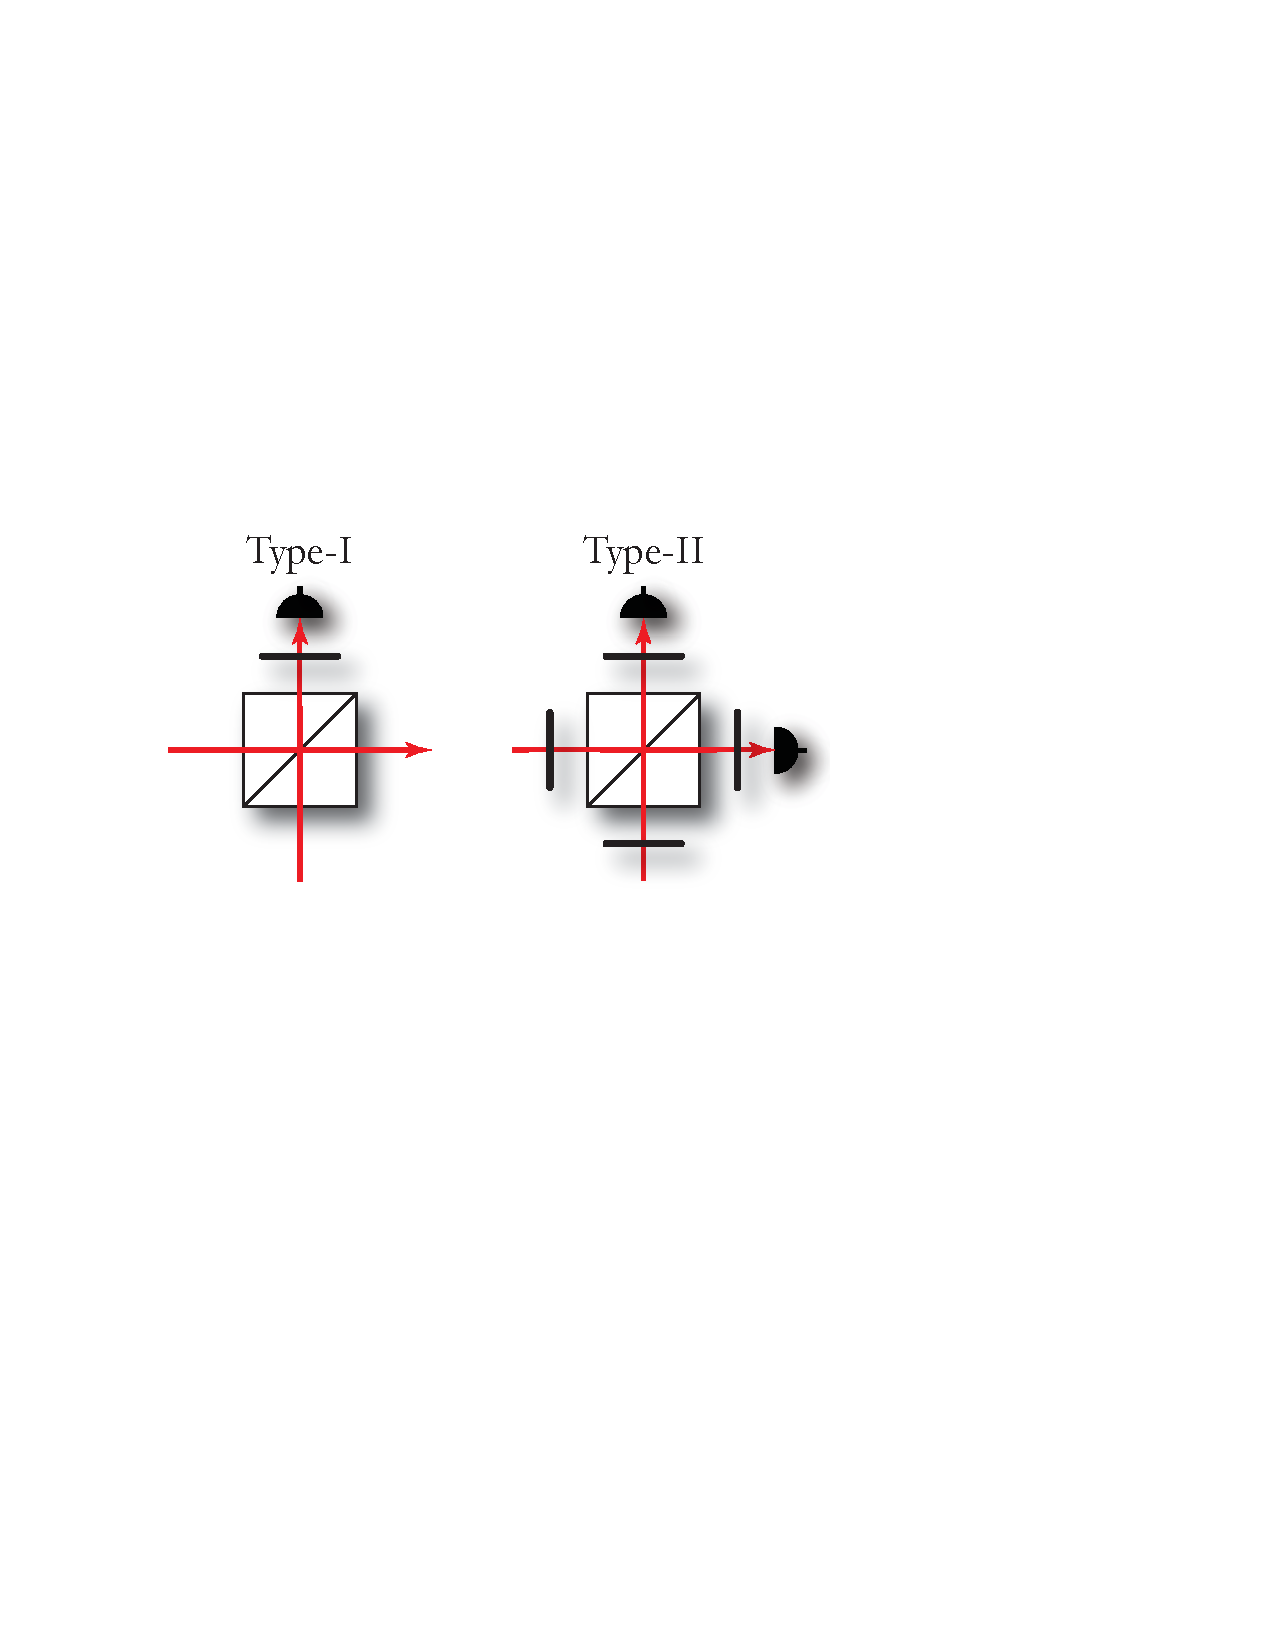
\includegraphics[clip=true, width=0.4\textwidth]{fusion_gates}
\captionspacefig \caption{Linear optics cluster state fusion gates for polarisation-encoded photons. Both type-I and type-II gates employ a single polarising beamsplitter to mediate the entangling measurement. The black bars represent Hadamard gates in the polarisation basis (waveplates). The type-I gate only measures a single photon, the other freely exiting the gate, which forms a part of the final cluster state. The type-II gate consumes two photons. Because the type-I gate does not measure in coincidence, as per the type-II gate, it requires number-resolved photo-detection, whereas bucket detectors suffice for type-II.} \label{fig:fusion_gates}
\end{figure}

%
% Fusion Strategies
%

\subsubsection{Fusion strategies} \index{Fusion!Strategies}

If a large cluster state has $n$ edges in its graph, single-shot state preparation will succeed with probability $p^n$ if individual gates succeed with probability $p$, implying that on average $1/p^n$ attempts will need to be made until success. Clearly this exponentiality doesn't lend itself to efficient implementation.

Thankfully, cluster states needn't be prepared in a single shot, since individual gate failures do not destroy the entire graph, but rather only cause localised damage to the graph in the vicinity of the gate.

Despite their non-determinism, numerous authors have examined approaches for efficiently preparing arbitrarily large cluster states using these destructive, non-deterministic gates \cite{nielsen, kieling, rohdebarrett, kokBuffer, ???}. We refer to these schemes as `fusion strategies' -- simple algorithms for how to arrange qubits geometrically and the order in which to attempt bonding them.

These principles can be extended beyond LO to other schemes where entangling gates are inherently non-deterministic or sometimes fail in a heralded manner, e.g hybrid architectures (Sec.~\ref{sec:hybrid}), where a beamsplitter mediates entanglement via which-path erasure, but only successfully projects onto an entangled state with probability 1/2.

The key feature of all these fusion strategies is to employ `micro-clusters'\index{Micro-cluster states} as a primitive resource, which enable multiple bonding attempts between them via redundant vertices. We will now outline several of these schemes.

%
% Linear Clusters
%

\paragraph{Linear clusters}\index{Linear cluster states}

We begin with discussion of linear clusters as these are a particularly useful primitive resource for more advanced strategies. We briefly sketch out the formalism introduced by \cite{bib:RohdeBarrett07} for linear state preparation, which is applicable to a number of different variants of entangling gates.

A key observation was that although numerous strategies yield efficient state preparation, exact efficiencies are highly dependent on the ordering of bonding operations -- which clusters do we choose to bond together first?

Consider a non-deterministic KLM-type CZ gate\footnote{In reality, no one would use KLM-type gates for preparing cluster states, owing to their complexity compared to fusion gates. Rather, we use this gate for illustrative purposes, since its operation upon success and failure are very simple for exposition.}, which upon failure destroys its two input photons by measuring them in the computational $\hat{Z}$-basis, and leaves the number of qubits unchanged upon success and bonds them together.

To analyse the operation of such a non-deterministic protocol, we begin by defining a vector $\vec{n}_t$ at time $t$, which stores purely classical information. Specifically, the vector tells us how many clusters of every length we have stored in memory (except single-qubit clusters, which we assume `come for free'\footnote{As in beer.\index{Beer}}). For example, the second element of the vector tells us how many 3-qubit linear clusters we have in our possession.

We then define a strategy, $\mathcal{S}$\index{Fusion!Strategies}, for choosing clusters we have stored and bonding them together to form larger clusters. The strategy acts on our cluster vector and updates it accordingly,
\begin{align}\index{Update rules}
\vec{n}_{t+1} = \mathcal{S}(\vec{n}_t).
\end{align}
That is, the length vector can be thought of as a series of `buckets' containing clusters of different lengths, and the strategy simply probabilistically shuffles the contents of the buckets around each time it is applied. The process can be thought of as a random walk\index{Random walks}, guided by a probabilistic update rule. Fig.~\ref{fig:linear_cs_strategy} outlines the protocol.

\begin{figure}[!htbp]
	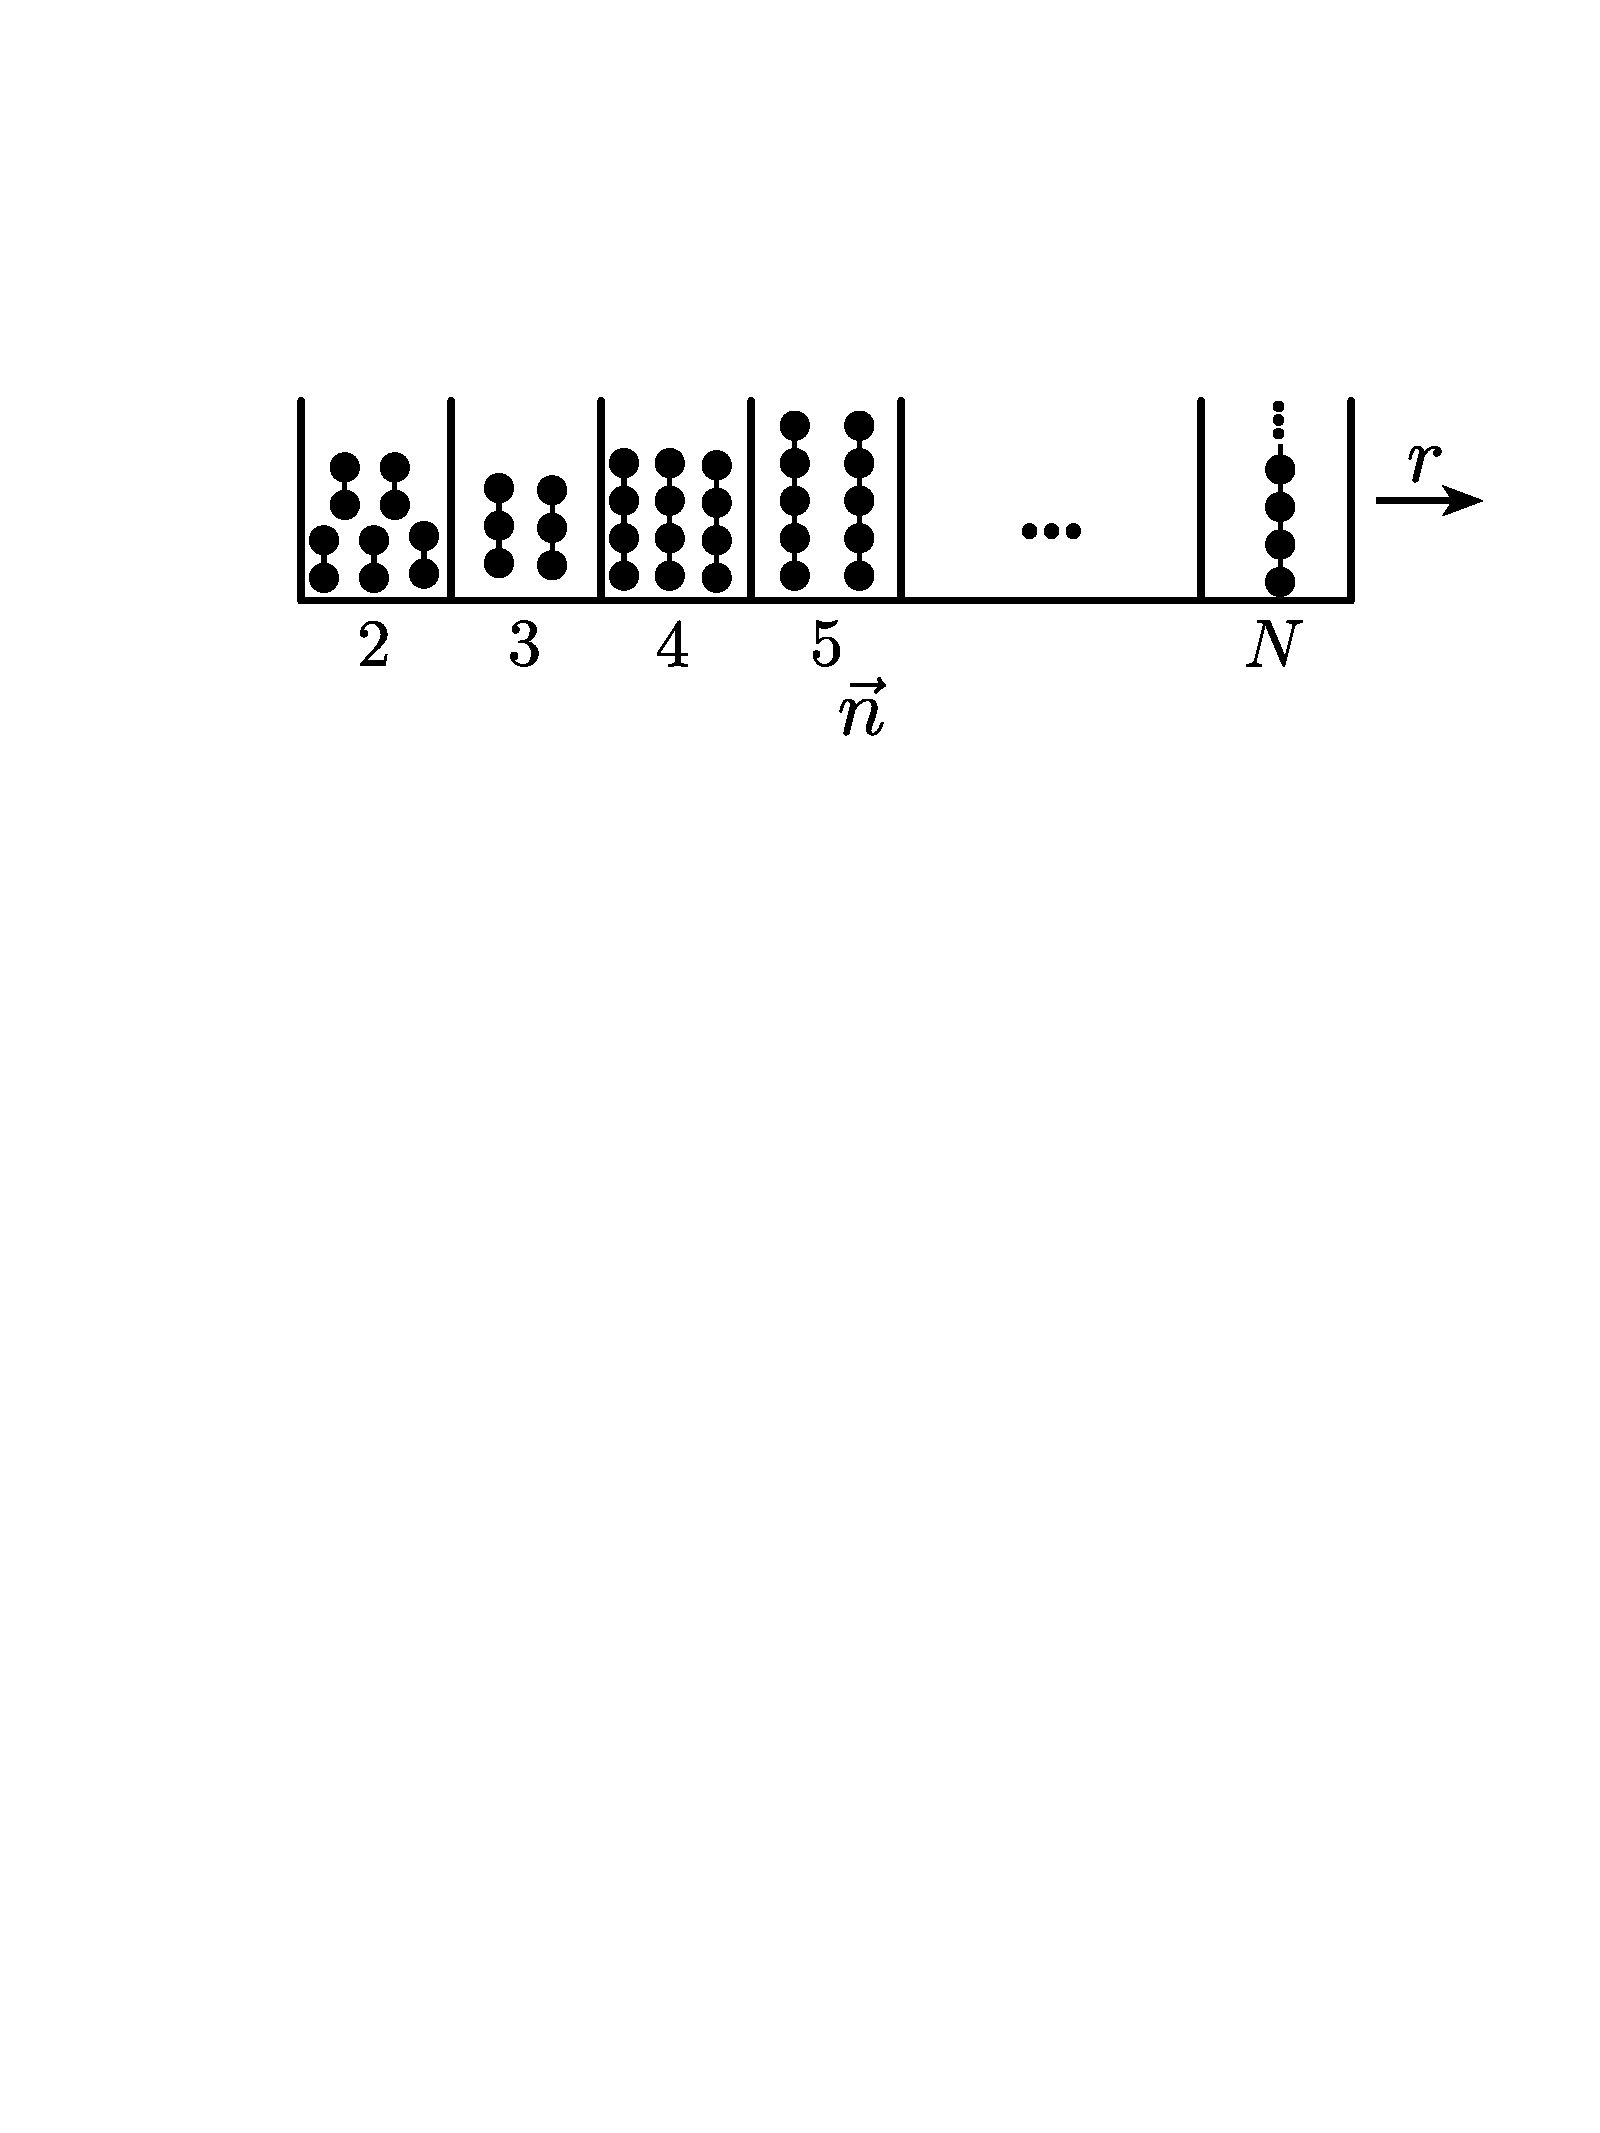
\includegraphics[clip=true, width=0.475\textwidth]{linear_cluster_state_strategies}
	\captionspacefig \caption{Protocol for preparing linear cluster states using non-deterministic entangling gates and quantum memory. Each `bucket' holds a resource of micro-clusters of a given length, represented by the vector $\vec n$. Beginning with a resource of single qubits we repeatedly attempt bonding operations between micro-clusters in the buckets, according to a fusion strategy, $\mathcal{S}$. Proceeding as a biased random walk, the contents of the buckets shuffle around until ultimately (hopefully) clusters of the target length $N$ are prepared and steadily flow out as output at rate $r$ clusters per update operation. We assume a free supply of single qubits as a resource.}\label{fig:linear_cs_strategy}
\end{figure}

The strategy description, $\mathcal{S}$, is also responsible for taking care of updating the elements of $\vec{n}$ according to an update rule, which dictates how many photons are lost or gained upon success or failure of the non-deterministic gate. For example, the CZ gate we have employed here for our toy model destroys two qubits upon failure, but upon success creates a cluster of length given by the sum of the lengths of the clusters acted upon by the gate.

We are then interested in the \textit{rate}\index{Cluster states!Preparation rate}, $r$, at which large clusters are output from the protocol. This is simply extracted by defining a single parameter which counts the number of clusters in $\vec{n}$ above some predetermined target length, and normalises it by the total time taken to reach that point. The rate parameter converges asymptotically for long runtimes. Formally, the rate of preparation is given by,
\begin{align}
r = \lim_{t\to\infty} \frac{N_t}{t},
\end{align}
where $N_t$ is the total number of clusters of length greater than the target length at time $t$. The preparation rate is bounded by \mbox{$0\leq r\leq1$}. If the rate $r$ converges to a positive, finite value in the limit of large $t$, this implies state preparation proceeds in linear time and is therefore efficient.

This completes the theoretical analysis for different strategies and gate types, allowing us to explore different approaches tailored to different physical systems and their varying gate implementations.

One of the key outcomes was that a \textsc{Balanced} strategy\index{Balanced strategy} is optimal in terms of preparation rate. This is simply a strategy which preferentially always bonds clusters of equal length, beginning with the largest ones available. Asymmetric strategies, which bond clusters of differing lengths were found to be far less efficient.

Example simulated state preparation rate results are shown in Fig.~\ref{fig:linear_cluster_state_r} for various types of entangling gates and gate success probabilities.

\begin{figure}[!htbp]
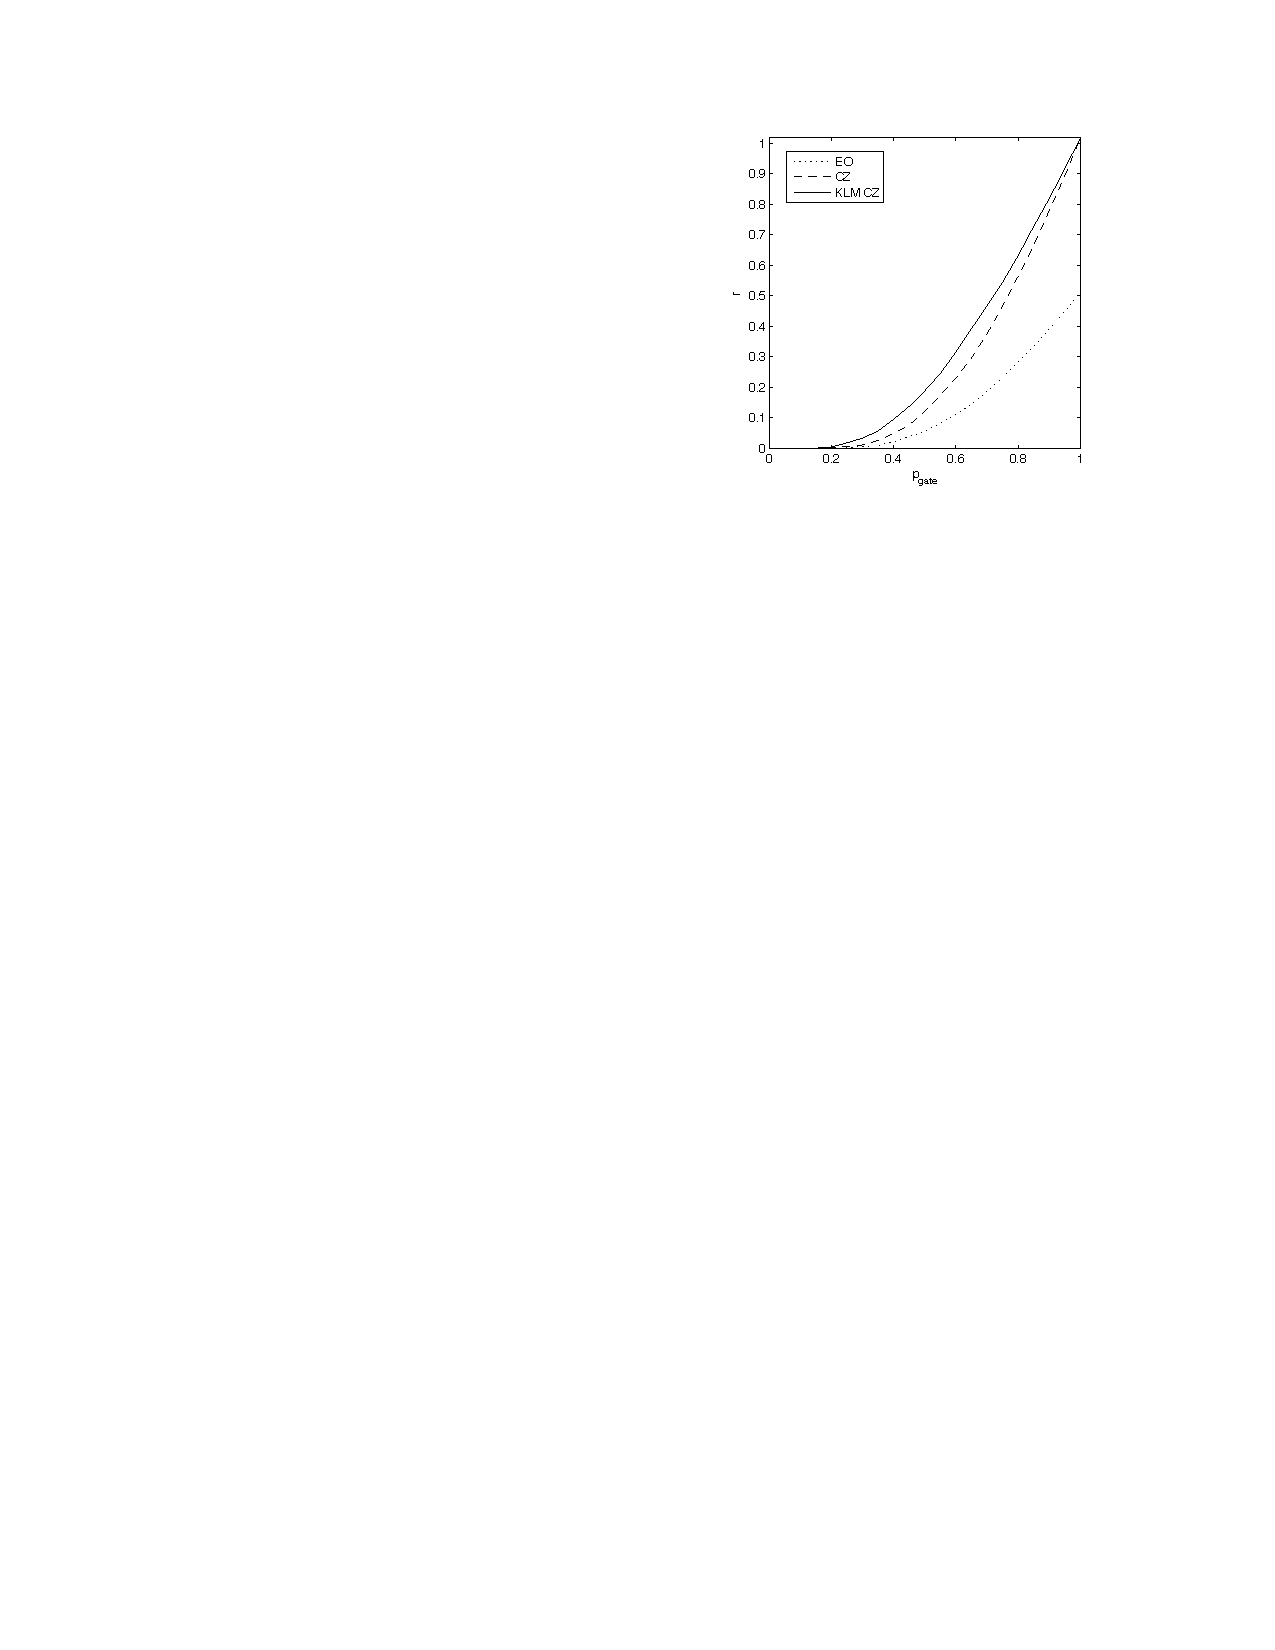
\includegraphics[clip=true, width=0.475\textwidth]{linear_cluster_state_rates}
\captionspacefig \caption{Linear micro-cluster preparation rates for three different types of entangling gates as described in \cite{bib:RohdeBarrett07}, against gate success probability, $p_\mathrm{gate}$. Here a \textsc{Balanced} fusion strategy is employed, whereby we only attempt to join clusters of equal length, always prioritising the largest ones available. This strategy was empirically found to perform better than any asymmetric strategies.}\label{fig:linear_cluster_state_r}
\end{figure}

%
% Lattice Clusters
%

\paragraph{Lattice clusters}\index{Lattice cluster states}

As we learnt from Sec.~\ref{sec:CSQC}, linear cluster states are not universal for quantum computation. What is required is lattices, where the rows and columns respectively map to logical qubits and time in the circuit model. There are numerous approaches one could employ to assemble such lattice clusters using non-deterministic gates, however the easiest to treat for illustrative purposes is to take a resource of linear clusters, prepared as described earlier, and weld them together according to some algorithm, enabling more complex two-dimensional topologies.

The central strategy is similar as for linear clusters -- we construct recyclable micro-clusters, which enable multiple bonding attempts, since gate failures only cause localised damage. The key difference now is that these redundant vertices must emanate in multiple directions so as to allow the more complex 2D topology.

Fig.~\ref{fig:micro_clusters} illustrates several topologies for micro-clusters, beginning with the linear micro-cluster that we employed previously for preparing 1D clusters, and two variations of micro-clusters that can be employed for 2D state preparation.

\if 2\pubmode
\begin{figure}[!htbp]
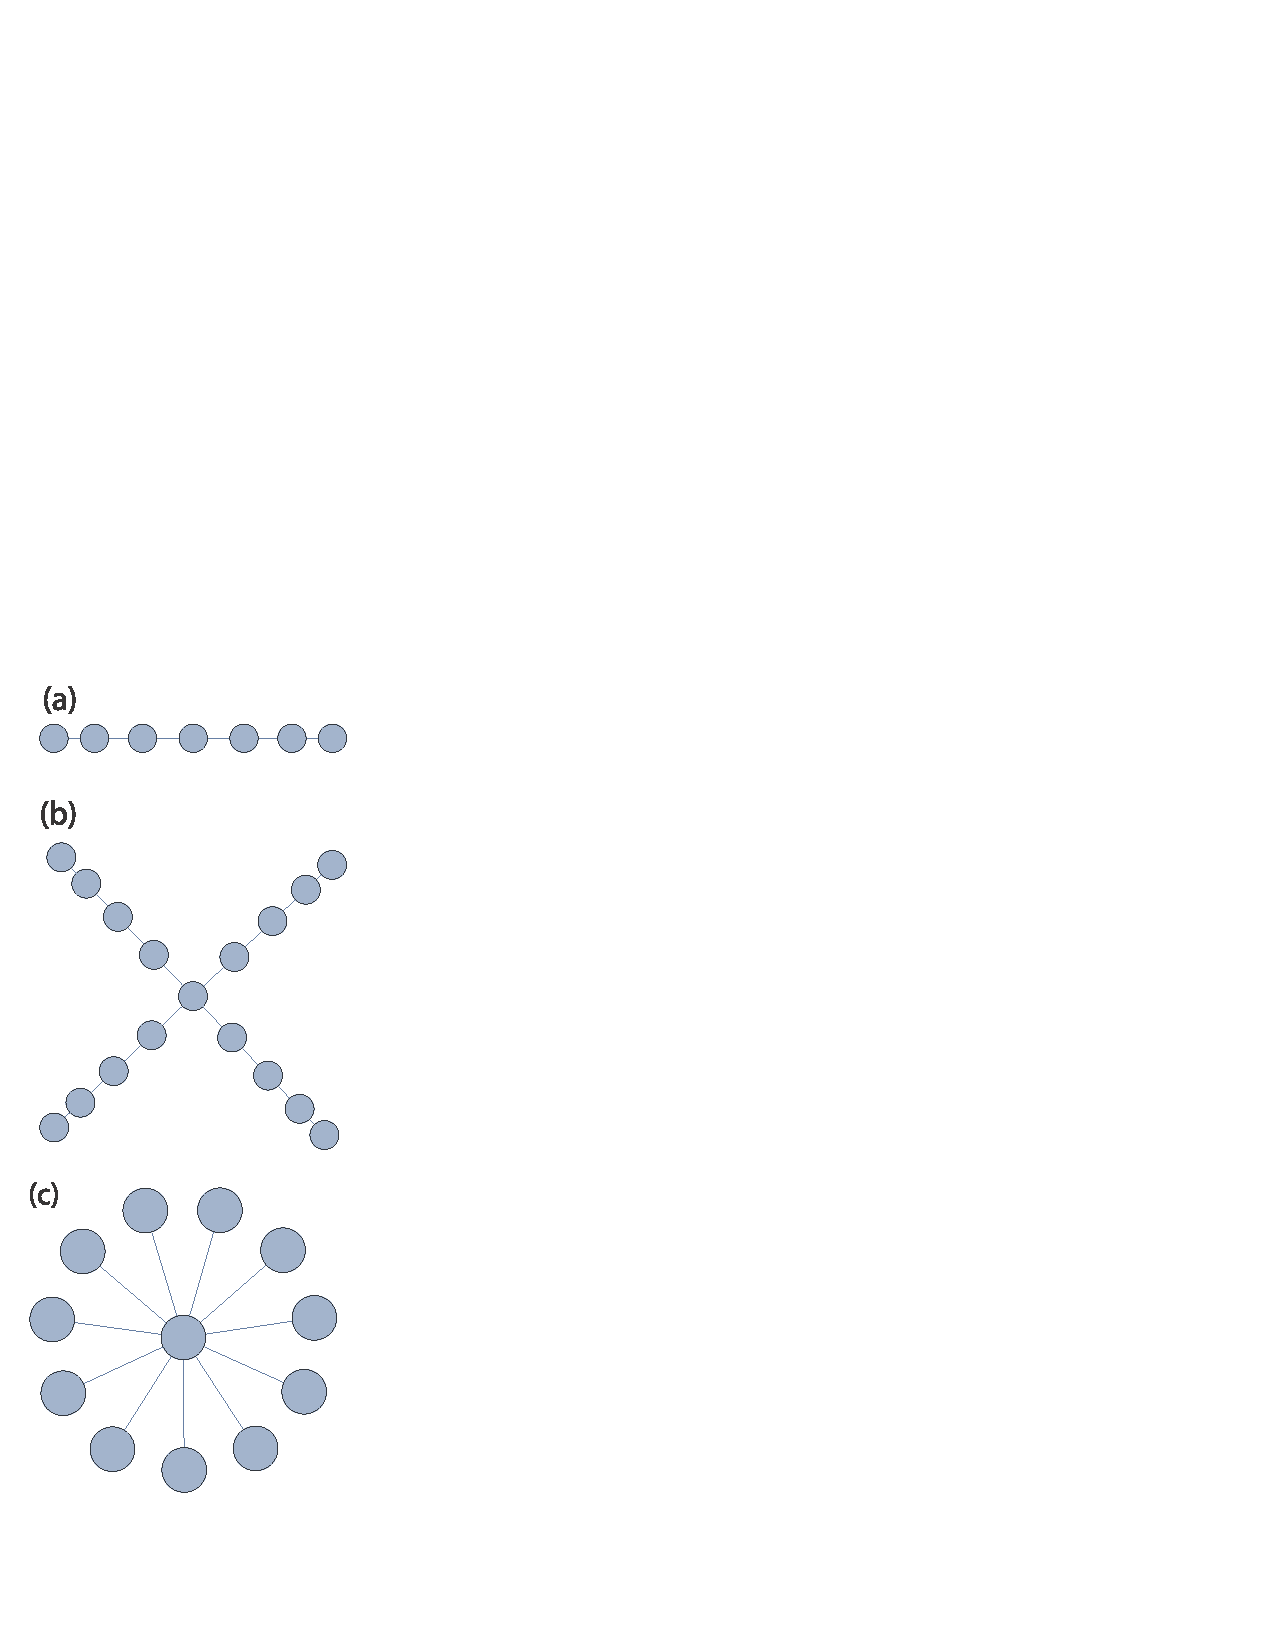
\includegraphics[clip=true, width=0.2\textwidth]{micro_clusters_long}
\captionspacefig \caption{(a) Linear, (b) plus ($+$), and (c) star micro-cluster states.}\label{fig:micro_clusters}\index{Linear micro-cluster states}\index{Plus micro-cluster states}\index{Star micro-cluster states}\index{Micro-cluster states}
\end{figure}
\else
\begin{figure*}[!htbp]
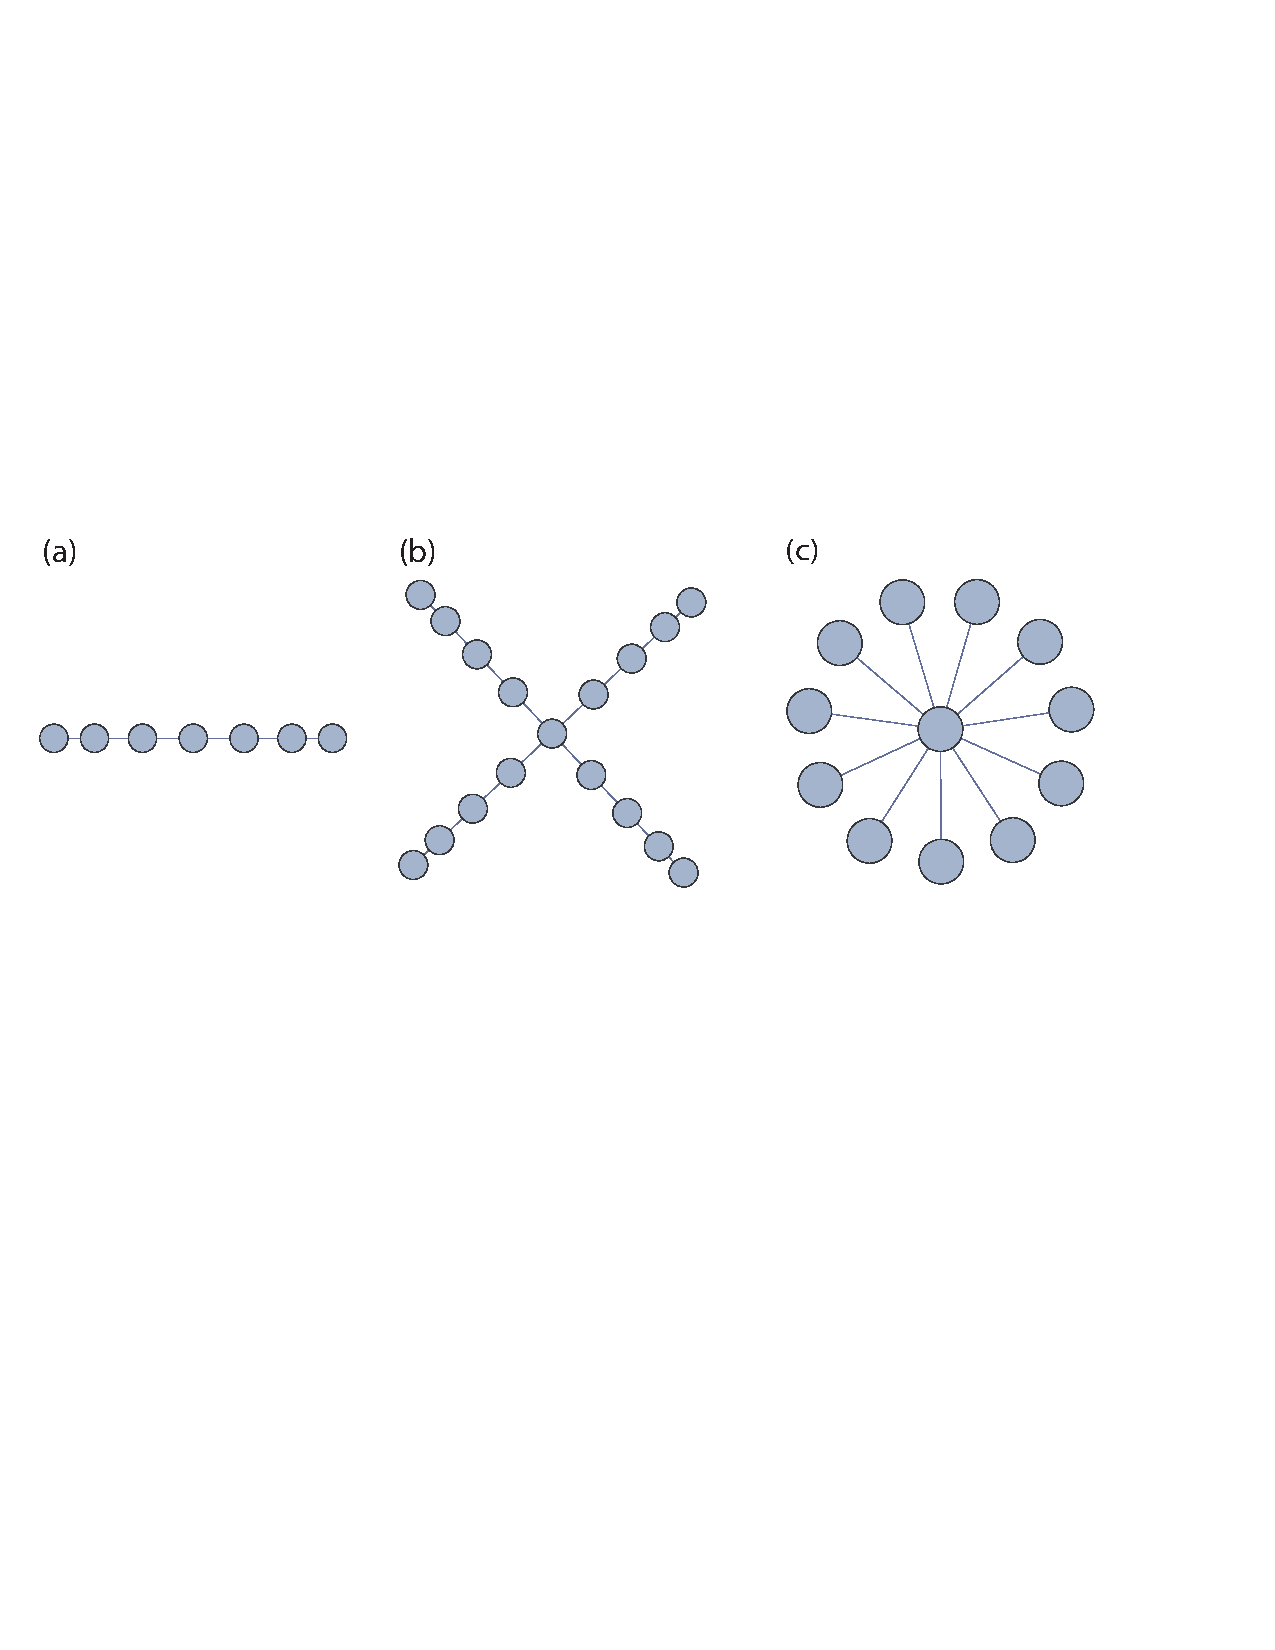
\includegraphics[clip=true, width=0.7\textwidth]{micro_clusters}
\captionspacefig \caption{(a) Linear, (b) plus ($+$), and (c) star micro-cluster states.}\label{fig:micro_clusters}\index{Linear micro-cluster states}\index{Plus micro-cluster states}\index{Star micro-cluster states}\index{Micro-cluster states}
\end{figure*}
\fi

The $+$-cluster\index{Plus micro-cluster states} simply comprises four linear clusters emanating in the four directions, welded together at a central vertex. It's self-evident how this is subsequently applied to 2D state preparation -- we lay out the $+$-clusters in a grid, and attempt nearest neighbour bonding in each direction for every neighbouring pair of micro-clusters.

The star-cluster\index{Star micro-cluster states} similarly allows multiple bonding attempts in each direction. But now the dangling bonds are not uniquely associated with a particular direction, and may therefore be utilised when bonding to a neighbouring micro-cluster in any direction. This implies a modest efficiency improvement, since leftover vertices in any given direction needn't be wasted upon a successful bond in that direction. However, these micro-clusters are not as efficient to prepare as the $+$-clusters, since they do not straightforwardly arise from two fused linear clusters, which are highly efficient to prepare. Rather they must be prepared via a sequence of repeated successful bonding operations to the central node, where a single gate failure destroys the entire state.

In addition to an efficiency improvement in terms of the number of required physical qubits, minimising the number of redundant qubits that must be removed via $\hat{Y}$ measurements upon completion of the bonding strategy has another key benefit -- error accumulation \cite{RohdeMunroEtal}. Whenever a cluster state qubit is measured, the action of any error process that acted on that qubit will be teleported to its neighbour(s). For example, if we measure the first qubit in a linear cluster, which was previously acted upon by a depolarising channel\index{Depolarising channel}, the depolarisation process will be teleported to the neighbouring second qubit in the cluster. Thus, with high levels of redundancy, although this increases our chances of successfully joining two micro-clusters, it similarly increases the accumulation of errors. There is therefore a direct tradeoff between two undesirable error mechanisms -- gate failure, and logical errors. This tradeoff must be carefully managed in a real-world implementation.

Having made this observation about error accumulation, is there a topology that is optimal? Yes there is -- the so-called snowflake cluster, shown in Fig.~\ref{fig:snowflake_graph}. He we take the $+$-cluster topology and replace the linear clusters emanating in each direction with binary tree graphs of some depth, $d$. This variation of micro-clusters has been studied in great detail both in optical and non-optical contexts \cite{SimonBenjaminPapers}.

The endpoints (leaves) of each tree now provide the bonding opportunities for joining two neighbouring micro-clusters. There are $O(2^d)$ such opportunities. The bonding attempts proceed as expected, always exploiting the trees' outermost leaves.

Now the key feature is that when two sub-trees are successfully bonded via their leaves we do not need to measure out \textit{all} the leftover redundant vertices to reduce the graph to the desired residual topology. Instead we can `prune' away entire sub-trees by performing $\hat{Z}$ measurements at the base of their trunks. All vertices above the trunk will thereby be detached from the graph and needn't all be individually measured. Correspondingly, any error processes that had acted on the pruned vertices will not be teleported onto the main cluster, only the measurements acting on the trunks will contribute.

\begin{figure}[!htbp]
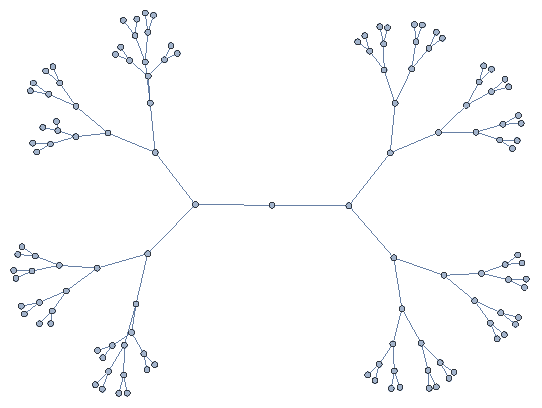
\includegraphics[clip=true, width=0.475\textwidth]{microcluster_snowflake}
\captionspacefig \caption{Snowflake micro-cluster comprising a binary tree structure, with depth \mbox{$d=7$}. Multiple copies of this micro-cluster can be placed side-by-side and fused together via attempting to bond the most outward available leaf qubits from neighbouring clusters. The tree structure allows excess qubits to be `pruned' via their trunks rather than leaves, bypassing the need to measure out every single leftover qubit, as is the case, for example, for $+$-clusters. This reduces the number of required pruning measurements from linear to logarithmic, similarly reducing the accumulation of errors associated with pruned qubits.} \label{fig:snowflake_graph}\index{Snowflake micro-cluster states}
\end{figure}

Formally, for a linear subgraph of length $n$, there will be $O(n)$ leftover redundant qubits on average, which must \textit{all} be measured out using $\hat{Y}$ measurements. Thus, the residual state will have accumulated the action of $O(n)$ independent error processes. On the other hand, for a snowflake subgraph, the trees' depth scales as \mbox{$d=O(\log n)$}, and therefore at most \mbox{$O(\log n)$} qubits must be measured to prune away unwanted branches. Fig.~\ref{fig:snowflake_pruning} presents an example of how the pruning process works.

\begin{figure}[!htbp]
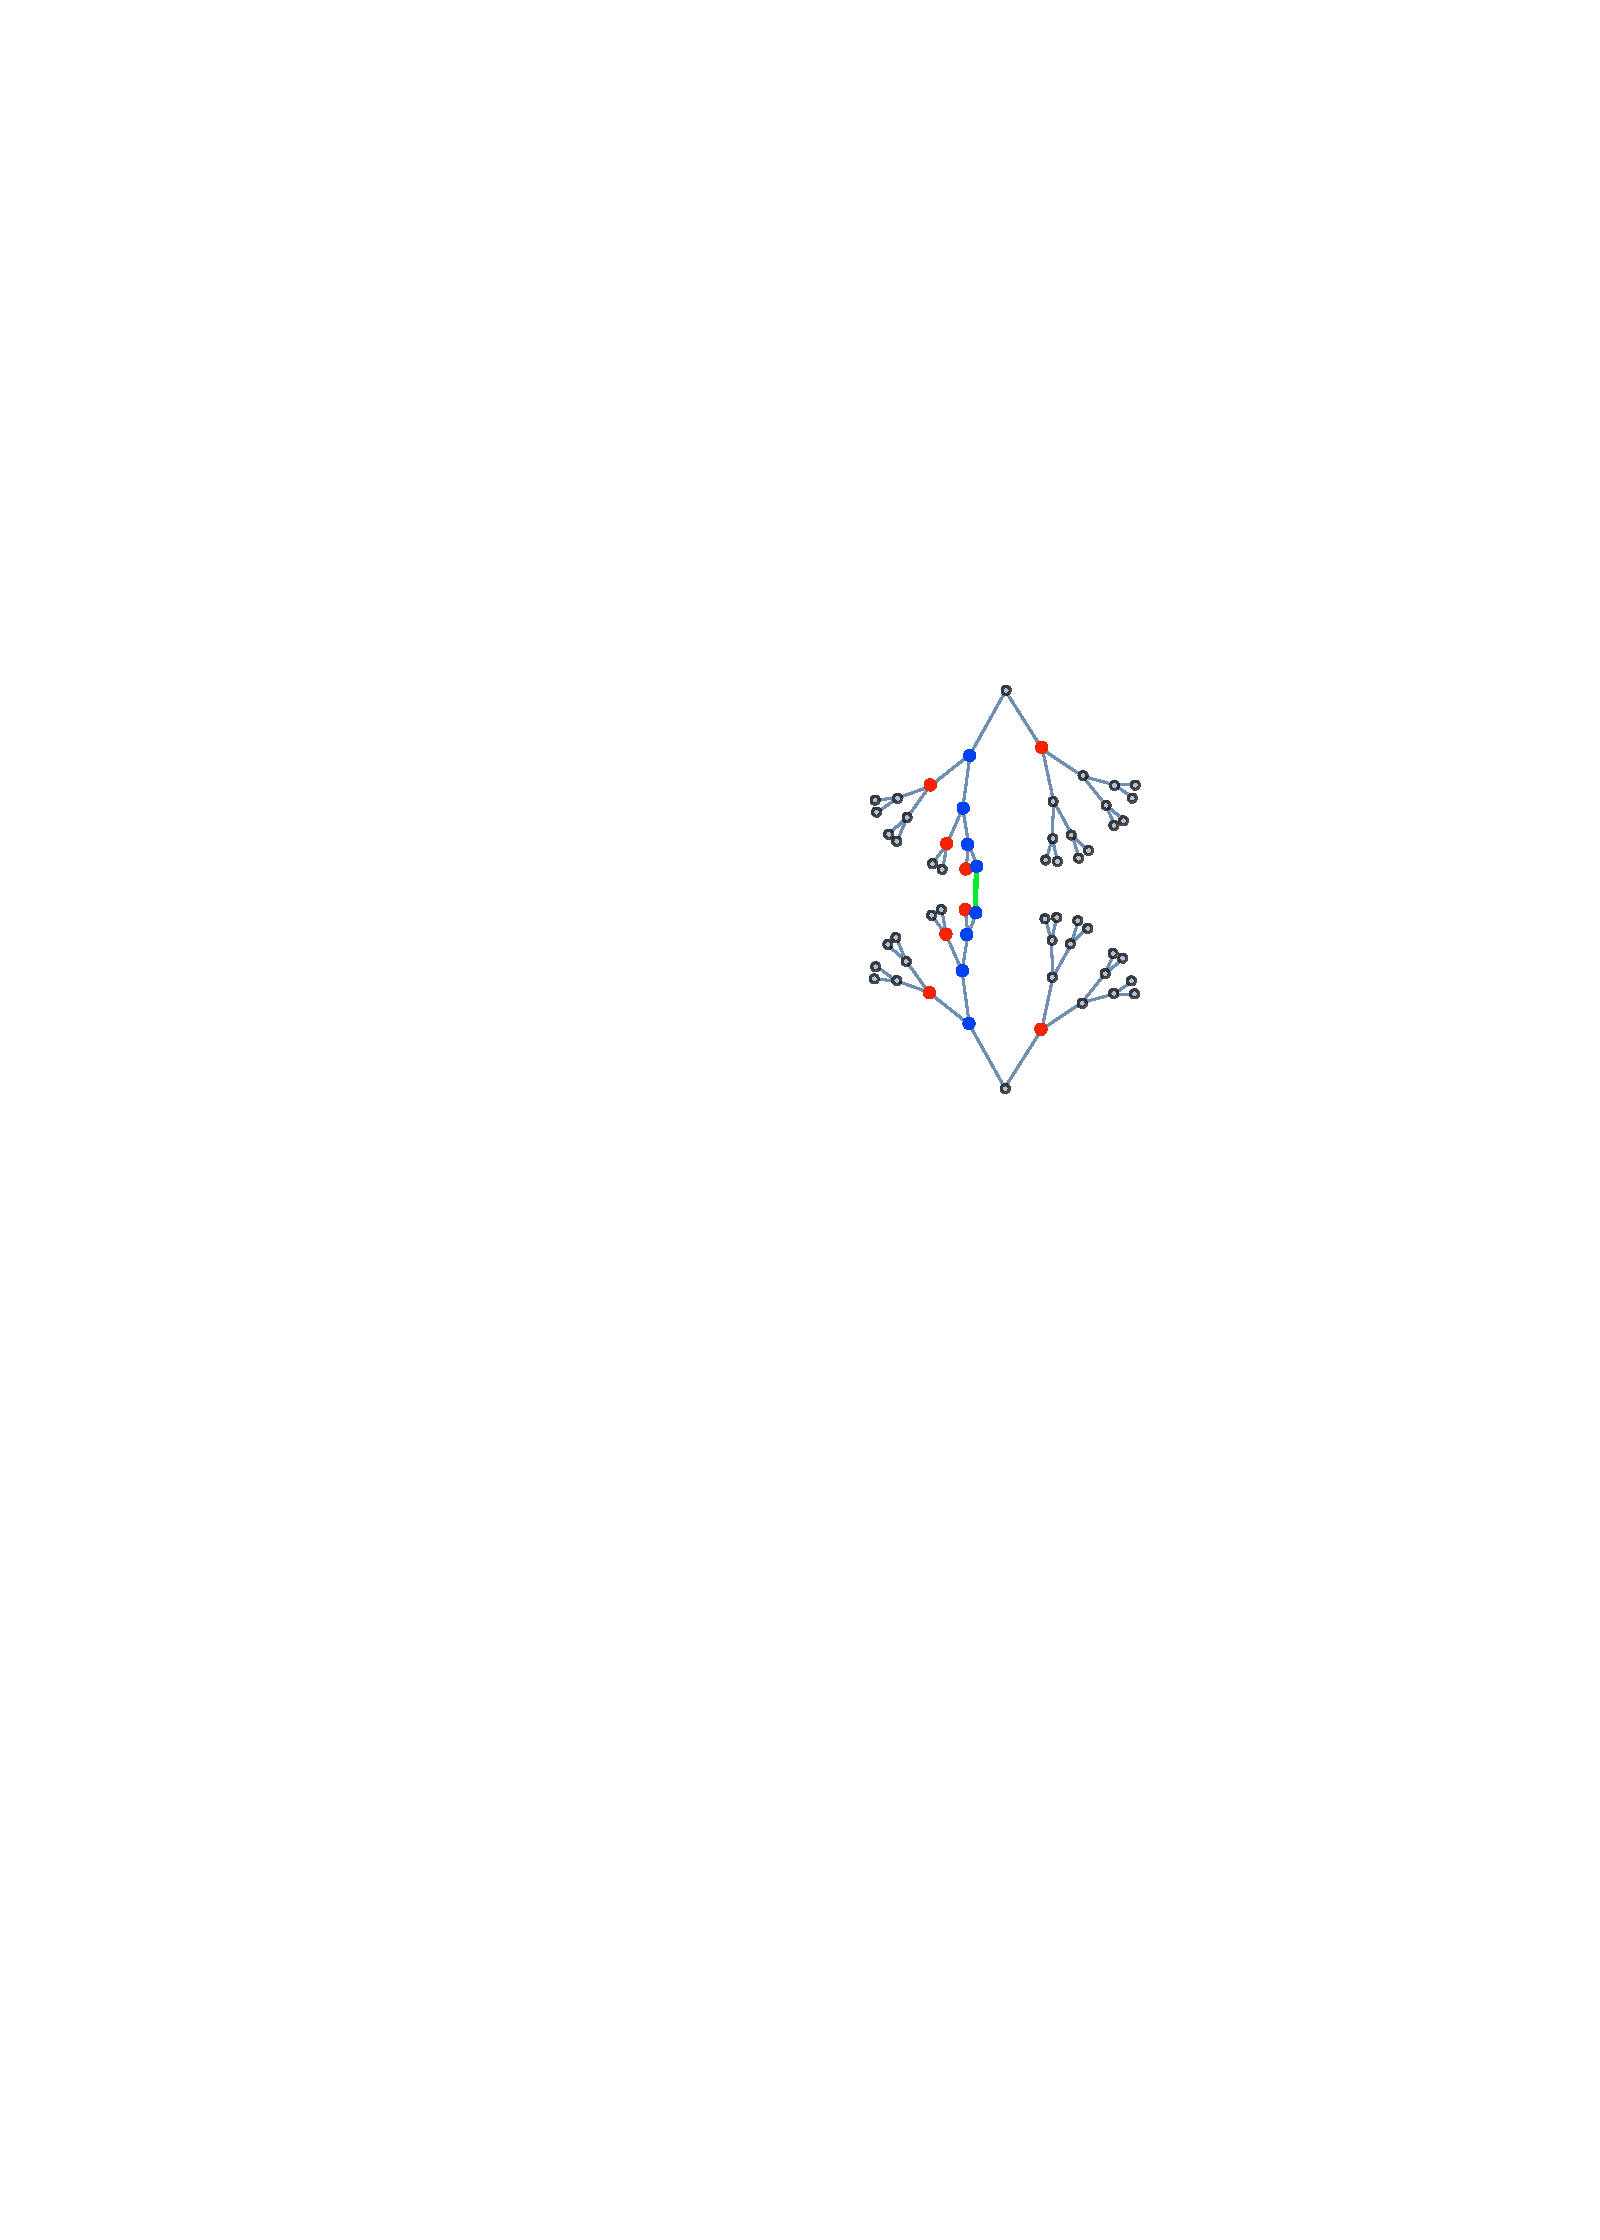
\includegraphics[clip=true, width=0.35\textwidth]{snowflake_pruning}
\captionspacefig \caption{Pruning snowflake micro-clusters\index{Snowflake micro-cluster states} upon successful fusion of their outer leaves. Green indicates where the successful fusion operation took place. To remove all redundant nodes we measure the qubits marked in blue in the $\hat{Y}$-basis and the ones marked in red in the $\hat{Z}$ basis. This will discard all the other qubits marked in grey, modulo the two root qubits at the far top and bottom, which are left with a direct link between them. The total number of measured qubits scales logarithmically with the number of leaves.}\label{fig:snowflake_pruning}	
\end{figure}

Keeping in mind that for an error process with error rate $p$, the net probability of an error occurring for $m$ independent channels is \mbox{$1-p^m$}, thus reducing $m$ from linear to logarithmic is highly favourable in terms of the accumulation of errors.

%
% On-Demand Cluster State Preparation
%

\paragraph{On-demand cluster state preparation}\index{On-demand cluster state preparation}

A beautiful feature of the cluster state model is that the entire cluster needn't be prepared in its entirety for computation to proceed. Instead the state can be grown via the fusion of additional qubits on-demand as the computation proceeds. This arises simply because all the entanglement in the graph is nearest neighbour only, i.e very short-range. So long as a gate failure doesn't lay its fingers on the leftmost column of qubits in the cluster we are in business. This means fewer quantum memories are required, which are very challenging optically. In non-optical, specifically matter qubit systems, this additionally means that physical qubits can be reused on-the-fly.

The computation therefore proceeds as alternating applications of: (1) measuring the leftmost column of physical qubits to evolve the computation by a single step; (2) bond on a new column of qubits to the rightmost column. The qubits in between the left and rightmost columns act as a buffer to give us some leeway when bonding operations fail. The architecture is shown in Fig.~\ref{fig:on_demand_cs}.

\begin{figure}[!htbp]
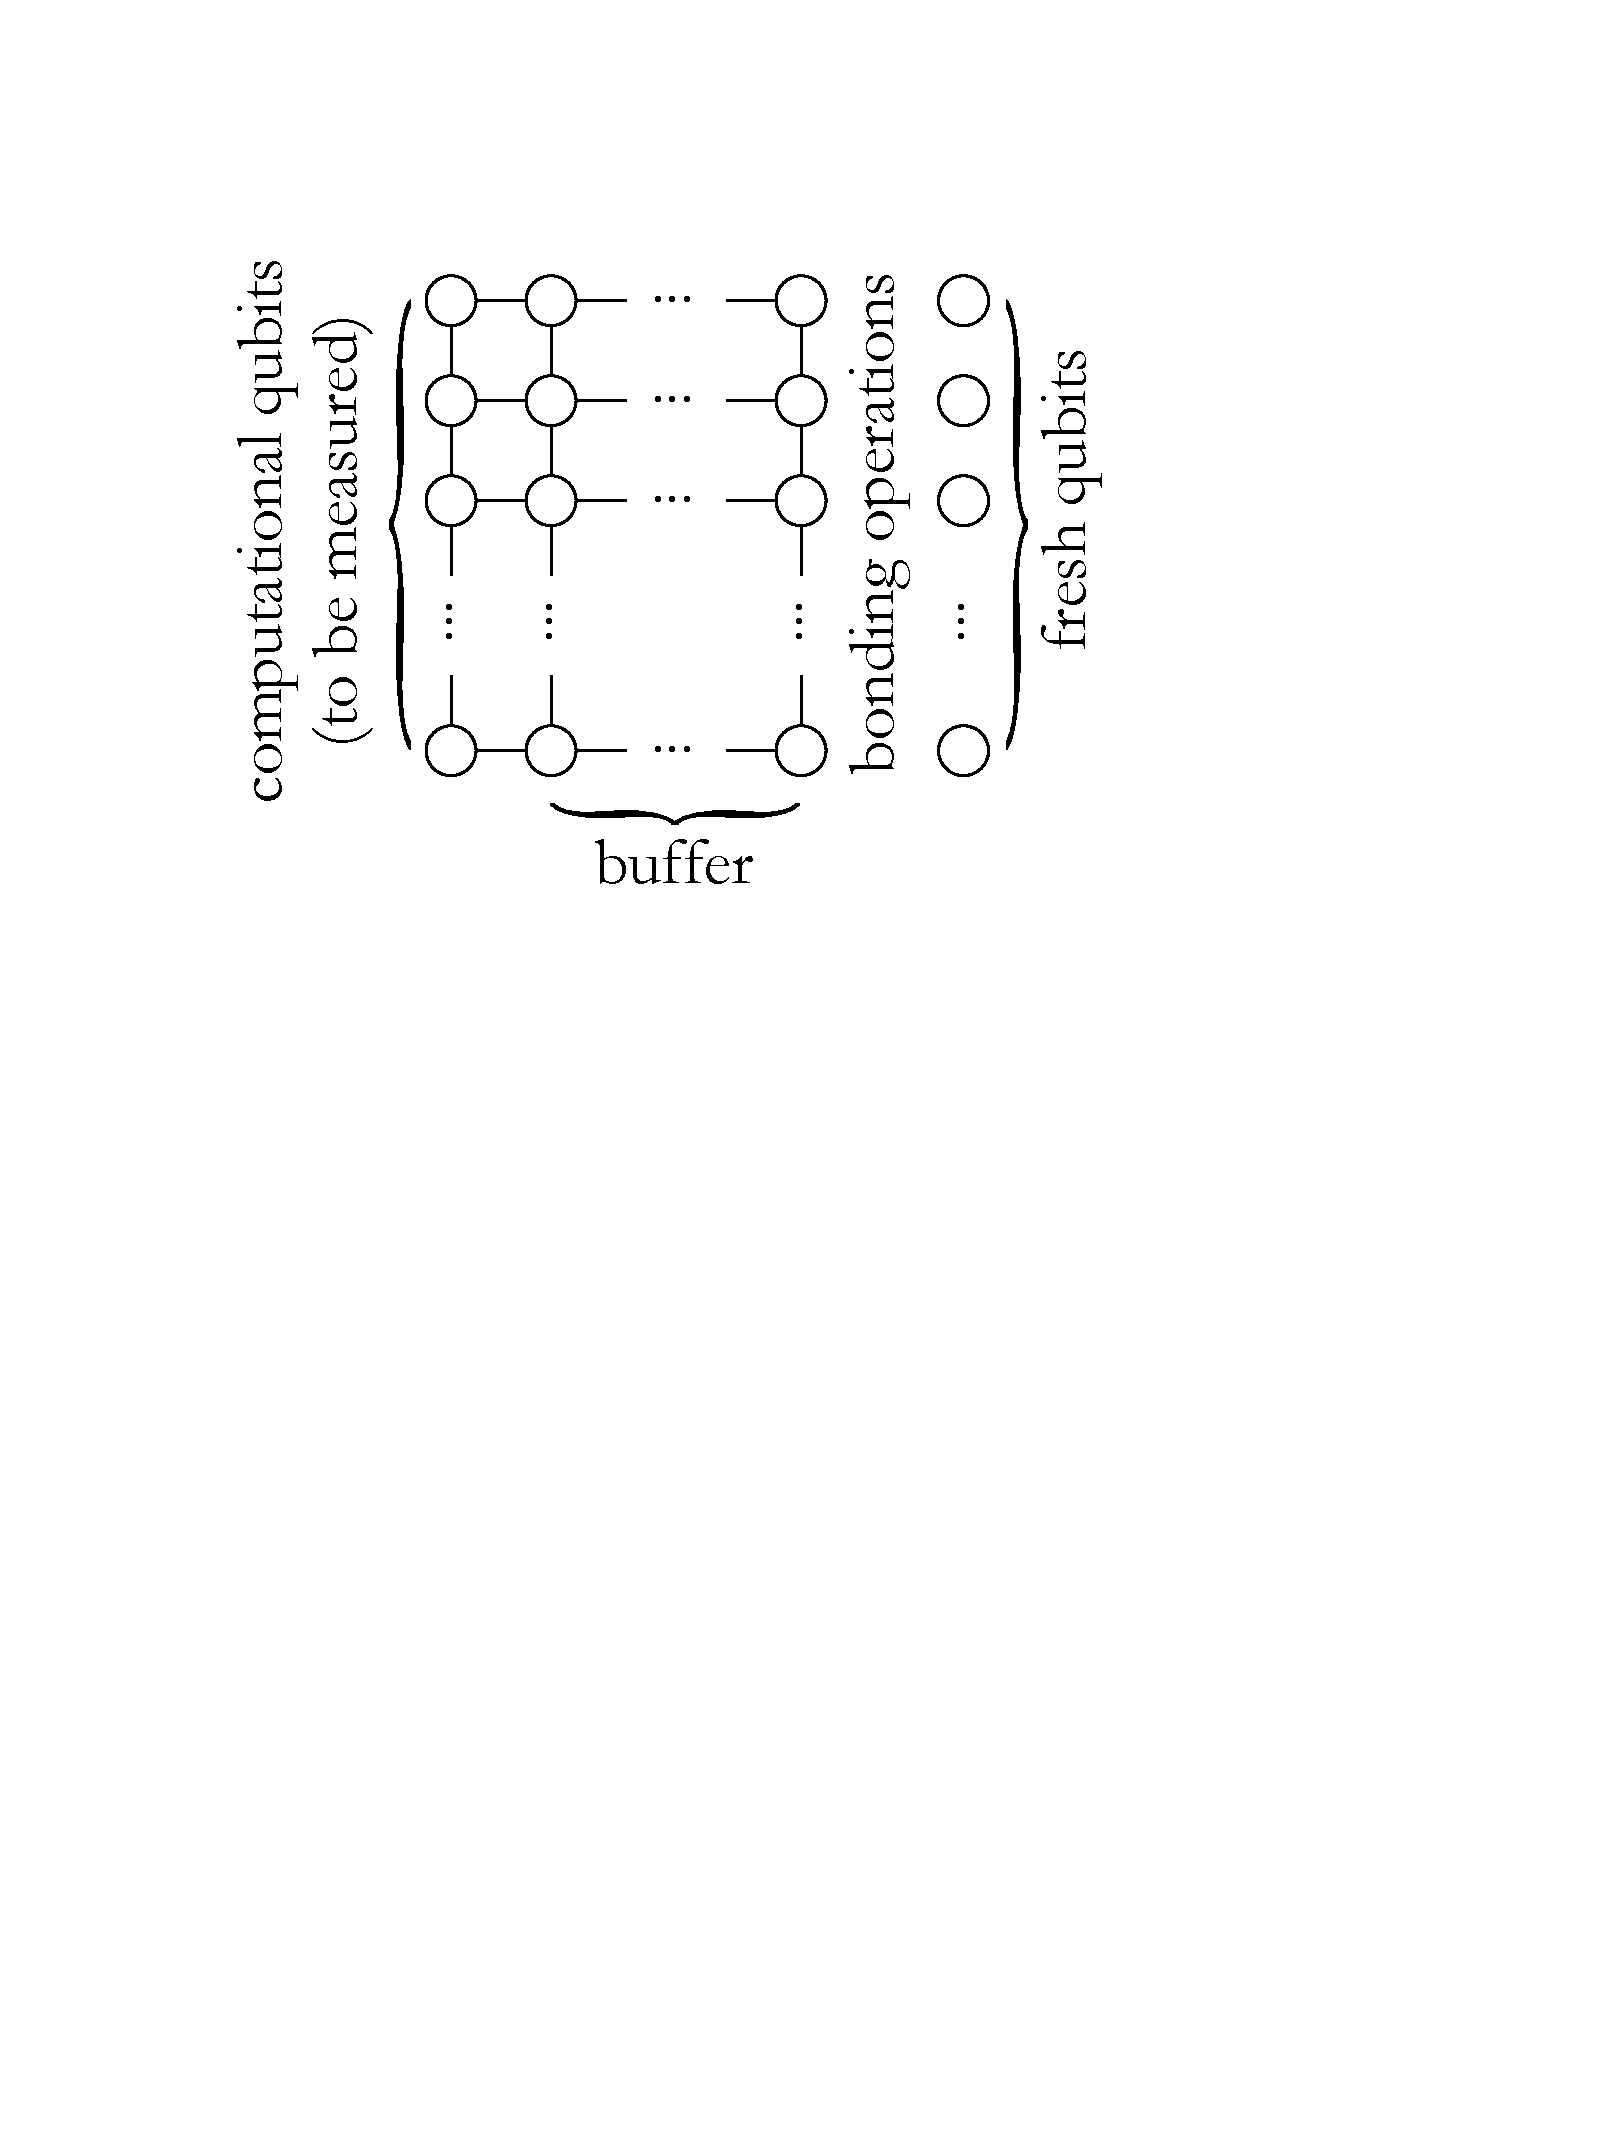
\includegraphics[clip=true, width=0.475\textwidth]{on_demand_cluster_states}
\captionspacefig \caption{On-demand cluster state preparation. Every time a column of computational qubits are measured away from the lefthand side, thereby evolving the computation by a single step, we dynamically bond on a fresh column of qubits to the righthand side. The buffer in between provides the redundancy necessary when using non-deterministic gates.}\label{fig:on_demand_cs}
\end{figure}

\cite{KokBuffer} performed an analysis of this approach in the optical context and found that high-depth MBQC can be efficiently implemented using non-deterministic entangling operations, with significantly reduced quantum memory requirements compared to full in-advance state preparation.

In addition to technologically simplifying the architecture by reducing the number of required quantum memories, physical qubits are in existence within the computation for substantially reduced periods of time, since they are only prepared on-demand. This correspondingly reduces error rates.

%
% Weak Cross-Kerr Non-Linearities
%

\subsection{Weak cross-Kerr non-linearities} \index{Weak cross-Kerr non-linearity quantum computation}

More recently, as an alternative to using post-selection to simulate strong optical non-linearities, it was shown that by introducing strong coherent states, the strength of a cross-Kerr optical non-linearity can be effectively amplified, allowing even very weak non-linearities to be employed for deterministic entangling gate operations \cite{bib:Munro05}. However, such schemes are particularly sensitive to loss, with sensitivity increasing with the coherent amplitudes in the system, creating a direct tradeoff between effective non-linear interaction strength and susceptibility to loss.

\comment{To do! Bill Munro perhaps?}
\index{Quantum bus (Qubus)}

%
% Passive Linear Optics
%

\subsection{Passive linear optics} \label{sec:passive_LO} \index{Passive linear optics quantum computation}

While the KLM protocol (and subsequent improvements, e.g using cluster states) are universal for quantum computing, some of the key technological requirements are very challenging, and unlikely to be achieved in the short-term. However, simplified yet non-universal models for optical quantum computing can abandon some of the more challenging requirements, nonetheless implementing a restricted set of post-classical quantum computations. In particular, we consider protocols requiring only photon-number state preparation, passive linear optics evolution [as per Eq.~(\ref{eq:LO_unitary_map})], and photo-detection.

Optically, the two main contenders for this are multi-photon quantum walks \cite{bib:Aharonov93, bib:Aharonov01, bib:Kempe03, bib:Childs09, bib:Salvador12, bib:RohdeMultiWalk11} and \textsc{BosonSampling} \cite{bib:AaronsonArkhipov10, bib:RohdeIntroBS15}, both closely related in that they require only passive linear optics and single-photon states, whilst mitigating the need for active switching, quantum memory and dynamic fast-feedforward. Since, evidence has been presented that similar passive linear optics protocols may implement computationally hard problems using states of light other than photon-number states \cite{bib:RandBS, bib:RohdePhotAdd15, bib:RohdeDisp15, bib:RohdeCat15}.

These protocols involve nothing more than evolving multiple single-photon states through beamsplitter networks and measuring the output photo-statistics. This is equivalent to just taking the first stage of the KLM protocol shown in Fig.~\ref{fig:KLM_protocol}.

Both quantum walks and \textsc{BosonSampling} have been subject to extensive experimental investigation in recent years \cite{bib:PeruzzoQW, bib:Broome10, bib:Schreiber11b, bib:Owens11, bib:RohdeQWExp12, bib:Broome2012, bib:RohdeQWExp12, bib:Spring2, bib:Crespi3, bib:Tillmann4}.

Because these models are entirely passive, they can be made cloud-based very trivially: Alice prepares her permutation of single photons as the input state, sends it to Bob over the quantum network, who applies the passive operations before returning the state to Alice. In this case, no intermediate client/server interaction is required. Alternately, she could classically communicate a bit-string to Bob indicating the input photon-number configuration, in case she is unable to prepare it herself.

The \textsc{BosonSampling} and quantum walk models are based on single-photon encoding. However, passive linear optics could also be applied to other states of light. In particular, passive linear optics acting upon multi-mode coherent states implements the \textit{classical} computation of matrix multiplication.

%
% Boson-Sampling
%

\subsubsection{\textsc{BosonSampling}} \label{sec:BS} \index{Boson-sampling}

\textsc{BosonSampling} is the problem of sampling the output photon-number statistics of a linear optics interferometer fed with single-photon inputs. While not universal for quantum computing (in fact no one has any idea what to use it for at all!), there is strong evidence that it is a classically hard problem \cite{bib:AaronsonArkhipov10, bib:RohdeIntroBS15}.

The computational hardness of \textsc{BosonSampling} relates to the fact that the amplitudes in the output superpositions are proportional to matrix permanents, which are known to be \#\textbf{P}-hard\index{\#P} in general. This is believed to be a classically hard complexity class, even harder than \textbf{NP}-complete\index{NP \& NP-complete} in the complexity hierarchy, requiring exponential classical time to evaluate (see Fig.~\ref{fig:complexity_classes} for the believed complexity relationships). This yields computationally complex sampling problems.

%
% The Boson-Sampling Model
%

\paragraph{The \textsc{BosonSampling} model} \index{Boson-sampling}

For an $m$-mode interferometer, and input state,
\begin{align}
\ket\psi_\mathrm{in} = \ket{T_1,\dots,T_m},
\end{align}
where there are $T_i$ photons in the $i$th input mode, the output superposition takes the form,
\begin{align}
\ket\psi_\mathrm{out} = \sum_S \gamma_{S,T} \ket{S_1,\dots,S_m},
\end{align}
where $S$ sums over all possible photon-number configurations at the output, of which there are,
\begin{align}
|S| = \binom{n+m-1}{n},
\end{align}
where there are $n$ photons in total in $m$ modes. It is assumed that,
\begin{align}
m=O(n^2),
\end{align}
which, for large $m$, puts us into the anti-bunched (i.e binary photon-number) regime with high probability\footnote{That is, we are unlikely to observe more than a single photon in any given output mode, placing us into a binary photo-detection regime. This condition has become known as the `bosonic birthday paradox' \cite{aaronson}.}, rendering non-number-resolved photo-detectors sufficient for physical implementation. However, this `no-collision' subspace remains exponentially large,
\begin{align}
|S_\mathrm{no\,collision}| = \binom{m}{n}.
\end{align}

The amplitudes $\gamma_{S,T}$ are given by,\index{Configuration amplitudes}
\begin{align}\label{eq:BS_perms}
	\gamma_{S,T} = \frac{\mathrm{Per}(U_{S,T})}{\sqrt{S_1!\dots S_m! T_1!\dots T_m!}},
\end{align}
and the associated configuration probabilities by,
\begin{align}
	P_{S,T} &= |\gamma_{S,T}|^2 \nonumber \\
	&= \frac{|\mathrm{Per}(U_{S,T})|^2}{S_1!\dots S_m! T_1!\dots T_m!}
\end{align}
where $\mathrm{Per}(\cdot)$ denotes the matrix permanent, and $U_{S,T}$ is a sub-matrix of $U$ -- the transfer matrix\index{Transfer matrices} associated with the particular input-to-output sample configuration -- obtained by taking $S_i$ copies of the $i$th row, and $T_j$ copies of the $j$th column of the linear optics unitary matrix $U$. For the purposes of the original complexity proof, the unitary is chosen randomly from the Haar-measure\footnote{The Haar-measure generalises the notion of a uniform distribution to higher-dimensional topologies than the real numbers, in this instance to the $\mathrm{SU}(n)$ group.}\index{Haar measure}, although it remains an open question as to what is the full class of unitaries that yield computationally hard problems.

\paragraph{The relationship to matrix permanents}\index{Permanents}

The observation that output probability amplitudes are related to matrix permanents as per Eq.~(\ref{eq:BS_perms}) is the most important one, as this is ultimately responsible for the computational hardness of the \textsc{BosonSampling} problem, since permanents are in general \textbf{\#P}-hard\index{\#P} problems, a classically inefficient complexity class.

The permanent of a square matrix is defined as\index{Permanents},
\begin{align}\label{eq:permanent}
\mathrm{Per}(A) = \sum_{\sigma\in S_n} \prod_{i=1}^n A_{i,\sigma_i},
\end{align}
which sums over $n!$ terms (super-exponential), where $S_n$ is the symmetric group, the group of permutations on $n$ elements, of which there are $n!$. Note the similarity with the definition for the matrix determinant\index{Determinants}, defines identically, but with the addition of an alternating $\pm$-sign in the terms. Despite this similarity, determinants reside in \textbf{P}, with an efficient classical algorithm. For this reason, Fermionic sampling\index{Fermionic sampling} yields an easy computational problem, since Fermionic sampling differs only in replacing the permanent with the determinant. The best-known classical algorithm for evaluating permanents by \cite{bib:RyserAlg} has exponential runtime,
\begin{align}
	O(2^n n^2).
\end{align}

To see how matrix permanents naturally arise in this setting, it is easiest to explain by example. In Fig.~\ref{fig:BS_2_comb} we illustrate a simple interferometer, fed with two photons. We wish to calculate the output amplitude of measuring a photon in each of the modes 2 and 3, given photons input at modes 1 and 2. To evaluate this amplitude we simply need to add up the amplitudes of all possible paths yielding the desired outcome. In this simple example this sum-of-paths\index{Sum-of-paths} is given by,
\begin{align} \label{eq:BS_2_ph_comb}
\gamma_{\{2,3\}} &= \underbrace{U_{1,2}U_{2,3}}_{\mathrm{don't\ swap}} + \underbrace{U_{1,3}U_{2,2}}_{\mathrm{swap}} \nonumber \\
&= \mathrm{Per} \left[ {\begin{array}{cc}
   U_{1,2} & U_{2,2} \\
   U_{1,3} & U_{2,3} \\
  \end{array} } \right],
\end{align}
from which it is immediately clear that the amplitude is given by the sum of \mbox{$2!=2$} paths\footnote{The number of paths scales as $n!$ in general, which corresponds to the $n!$ order of the symmetric group, $S_n$, in the definition of the permanent from Eq.~(\ref{eq:permanent}).}, the permanent of the \mbox{$2\times 2$} matrix obtained from taking the columns (rows) of $\hat{U}$ where a photon is present at the respective input (output) mode.

\begin{figure}[!htbp]
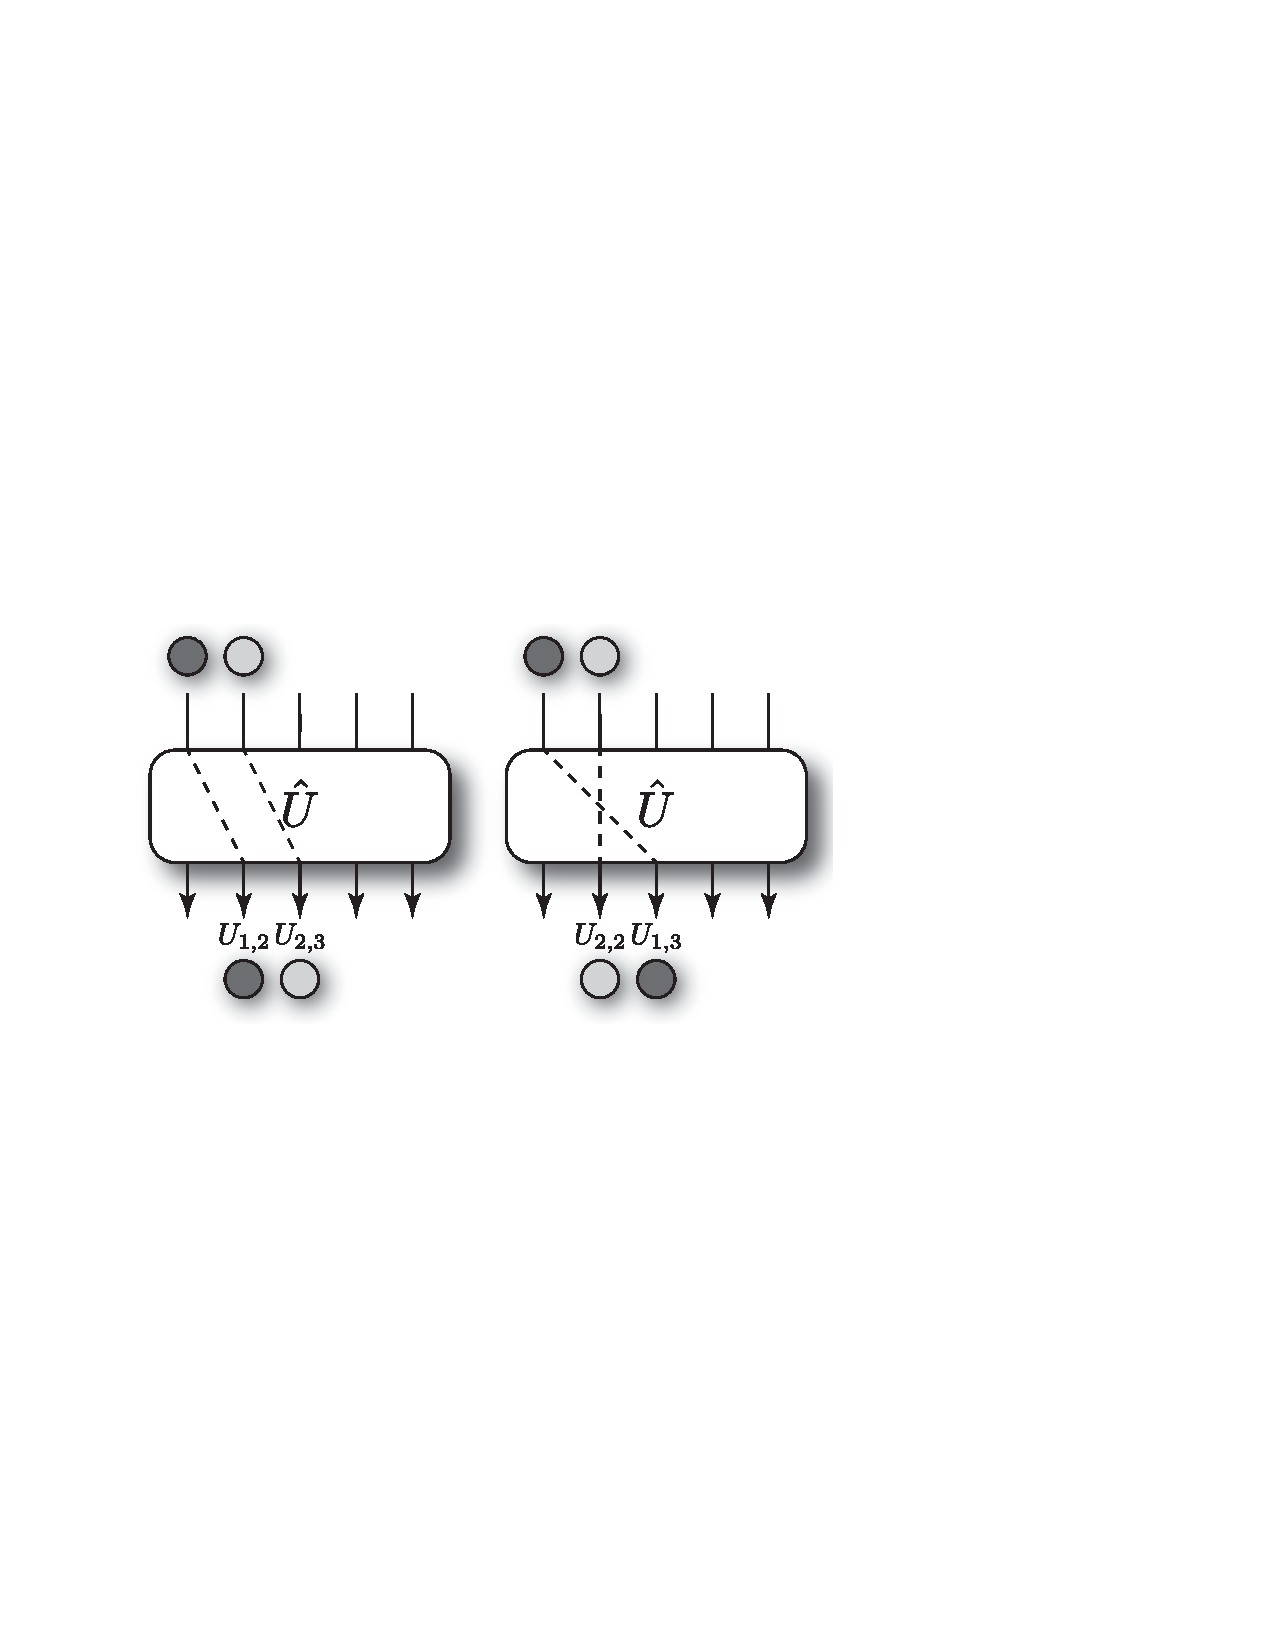
\includegraphics[clip=true, width=0.475\textwidth]{BS_2_photon_combinatorics}
\caption{A linear optics interferometer $\hat{U}$, fed with 2 single-photon inputs, one in each of the first two modes. To calculate the output amplitude of one photon in each of the modes 2 and 3, we sum the amplitudes of all possible paths consistent with that output. In this example there are only two such paths -- either both photons pass straight through, or they swap positions. This summation yields a \mbox{$2\times 2$} matrix permanent, given by Eq.~(\ref{eq:BS_2_ph_comb}).}\label{fig:BS_2_comb}	
\end{figure}

In Fig.~\ref{fig:BS_3_comb} we present to next most sophisticated example of an interferometer fed by 3 photons, for which the sum-of-paths\index{Sum-of-paths} has \mbox{$3!=6$} terms, given by,
\begin{align} \label{eq:BS_3_ph_comb}
\gamma_{\{1,2,3\}} &= U_{1,1}U_{2,2}U_{3,3} + U_{1,1}U_{3,2}U_{2,3} \nonumber \\
&+ U_{2,1}U_{1,2}U_{3,3} + U_{2,1}U_{3,2}U_{1,3} \nonumber \\
&+ U_{3,1}U_{1,2}U_{2,3} + U_{3,1}U_{2,2}U_{1,3}
\nonumber \\
&= \mathrm{Per} \left[ {\begin{array}{ccc}
   U_{1,1} & U_{2,1} & U_{3,1} \\
   U_{1,2} & U_{2,2} & U_{3,2} \\
   U_{1,3} & U_{2,3} & U_{3,3} \\
  \end{array} } \right],
\end{align}
and it is now clear upon inspection that the amplitude is given by a \mbox{$3\times 3$} matrix permanent.

\begin{figure}[!htbp]
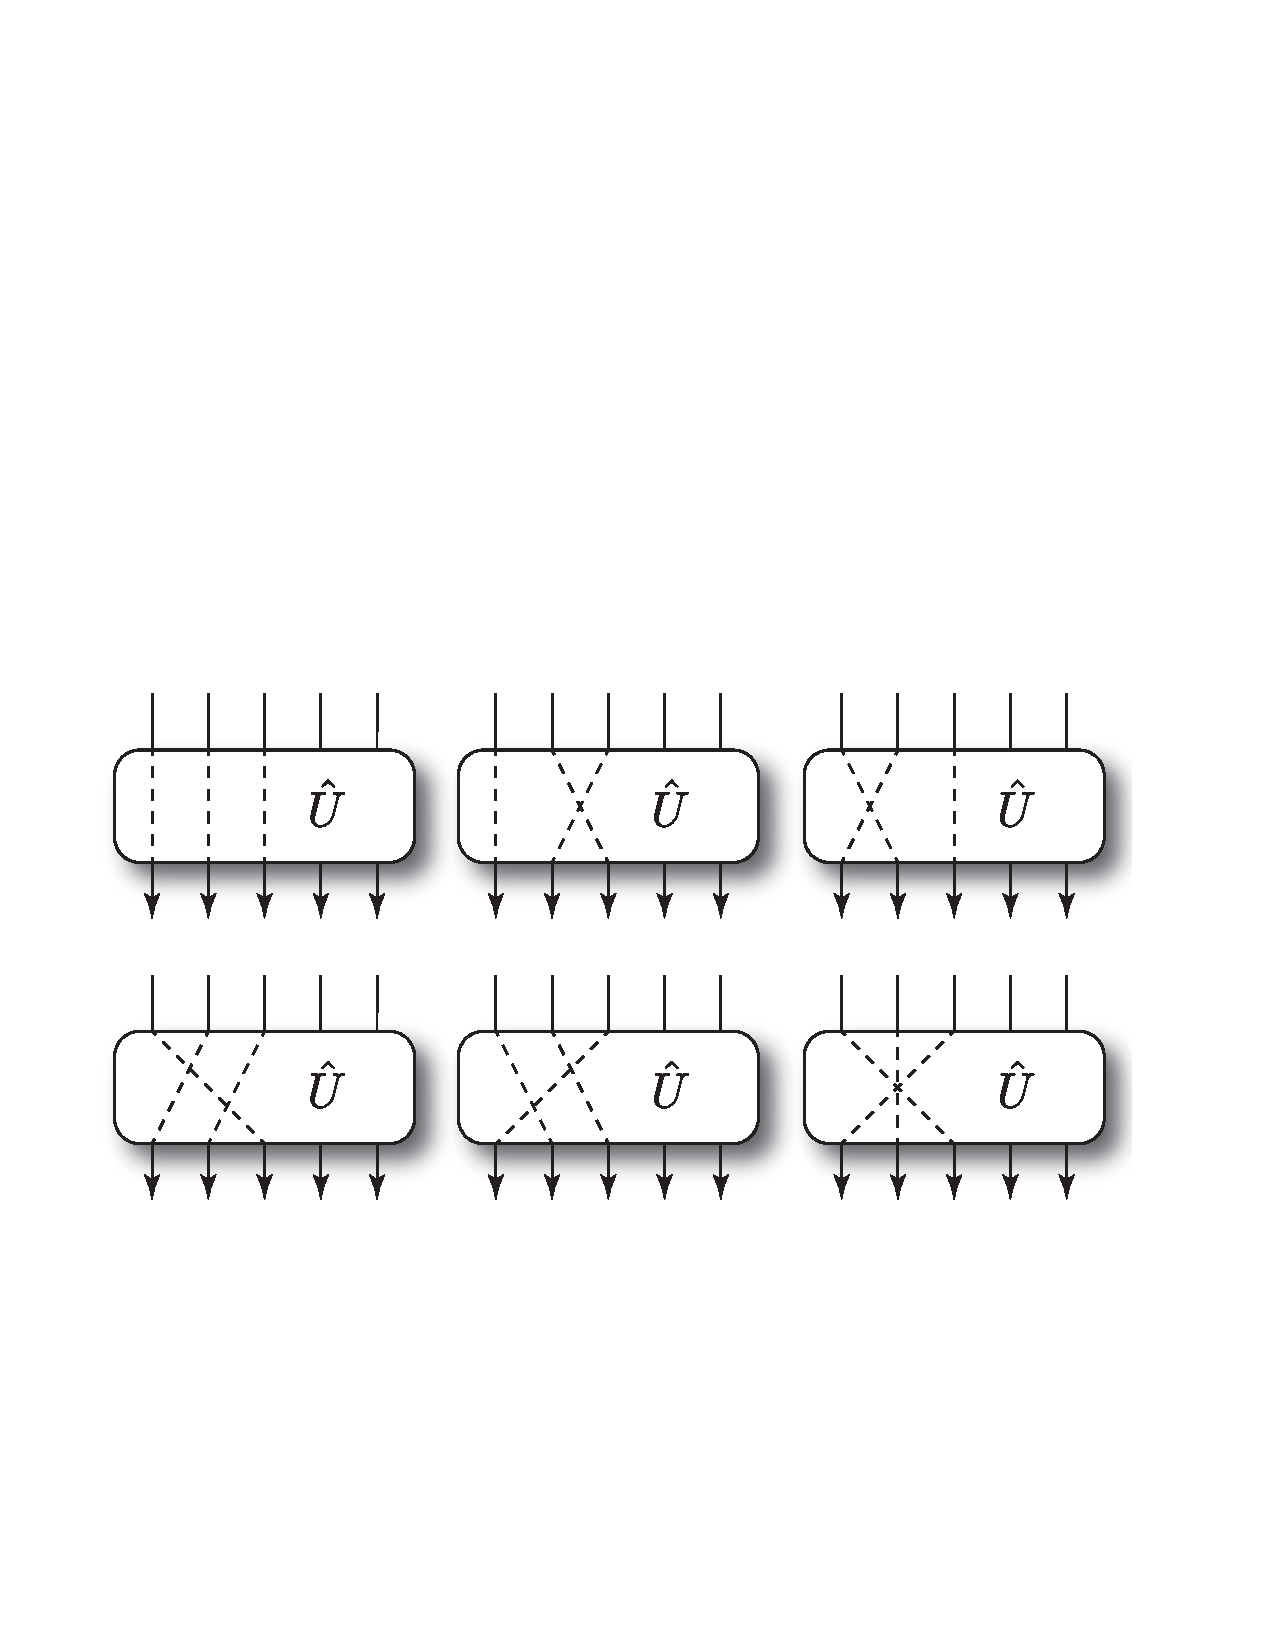
\includegraphics[clip=true, width=0.475\textwidth]{BS_3_photon_combinatorics}
\caption{A linear optics interferometer $\hat{U}$, fed with 3 single-photon inputs, in modes 1, 2 and 3. To calculate the output amplitude of one photon in each of the modes 1, 2 and 3, we sum the amplitudes of all possible paths consistent with that output. This summation yields a \mbox{$3\times 3$} matrix permanent, given by Eq.~(\ref{eq:BS_3_ph_comb}).}\label{fig:BS_3_comb}	
\end{figure}

\paragraph{Problem description}

The computational problem is simply to sample this probability distribution $P_{S,T}$, which the linear optics network can implement efficiently, but it is believed a classical computer cannot. The full model is shown in Fig.~\ref{fig:bs_model}.

\begin{figure}[!htbp]
\includegraphics[clip=true, width=0.35\textwidth]{BS_model}
\captionspacefig \caption{The \textsc{BosonSampling} model for non-universal linear optics quantum computing. $S$ (output) and $T$ (input) are represented in the photon-number basis. After application of the Haar-random linear optics unitary to the input multi-mode Fock state, the output superposition is sampled with coincidence photo-detection.} \label{fig:bs_model}
\end{figure}

For comparison, the equivalent classical protocol using distinguishable photons that evolve independently through the network would be described by,
\begin{align}
	P_{S,T} = \frac{\mathrm{Per}(|U_{S,T}|^2)}{S_1!\dots S_m! T_1!\dots T_m!},
\end{align}
which yields a classically efficient sampling problem. Thus, for \textsc{BosonSampling} the permanents are of complex-valued matrices, whereas for the equivalent classical problem the permanents are of positive real-valued matrices.

Very importantly, note that \textsc{BosonSampling} does \textit{not} let us efficiently \textit{calculate} matrix permanents. Rather, it samples across a distribution of an exponential number of permanents. This is because, for an exponentially large sample space, with only a polynomial number of measurement trials, we are unlikely to gain more than binary accuracy about individual amplitudes, which is insufficient for determining any particular permanent. It appears that God knows how to efficiently solve matrix permanents, but conspires against us such that we remain ignorant of them. \latinquote{Deus magnus est.}

The size of a boson-sampler required to exhibit post-classicality is under active debate, as has undergone much historical revision \cite{RohdeRalph}. But some recent estimates suggest that as many as \mbox{$n=50$} photons in \mbox{$m=2,500$} modes might be a rough guide for such a threshold \cite{NoSupBS_Montanaro}. Needless to say, this is already an extremely challenging technological goal, suggesting that although the \textsc{BosonSampling} problem is far simpler than universal LOQC, it is far from simple.

\textsc{BosonSampling} in the presence of various error models, such as loss, source non-determinism and mode-mismatch, has been extensively investigated \cite{bib:RohdeErrBS12, bib:RohdeSPDC13, bib:ScottLost16, bib:RohdeArbSpec15, bib:RandBS}. 

%
% Multiplexed Boson-Sampling
%

\paragraph{Multiplexed \textsc{BosonSampling}} \index{Multiplexed!Boson-sampling}

As discussed in Sec.~\ref{sec:single_phot_src}, SPDC is the most common present-day implementation of single-photon sources. However, despite their ready availability, they suffer from non-determinism, with single-photon heralding probability given by Eq.~(\ref{eq:SPDC_p_prep}). To improve upon this, multiplexed sources can be employed \cite{bib:RohdeSPDC13}, improving effective single-photon preparation probabilities asymptotically to unity, as given by Eq.~(\ref{eq:SPDC_multiplex}).

However, rather than employing a multiplexed SPDC source in place of each of the required $n$ single-photons, we can instead employ a larger multiplexer that routes \mbox{$N\gg n$} sources to $n$ modes, which is far more efficient than $n$ independent multiplexed single-photon sources.

The model is shown in Fig.~\ref{fig:multiplexed_bs}. We begin by operating $N$ SPDC sources in parallel. Clearly if $N$ is sufficiently large with respect to $n$, it becomes asymptotically certain that at least $n$ photons will be heralded. When this occurs, the successfully prepared $n$ photons -- in whatever configuration they happen to occur -- are routed to the first $n$ modes of the \textsc{BosonSampling} interferometer $\hat{U}$ by the multiplexer (which is classically controlled by the SPDC heralding outcomes), and the protocol proceeds as usual.

\begin{figure}[!htbp]
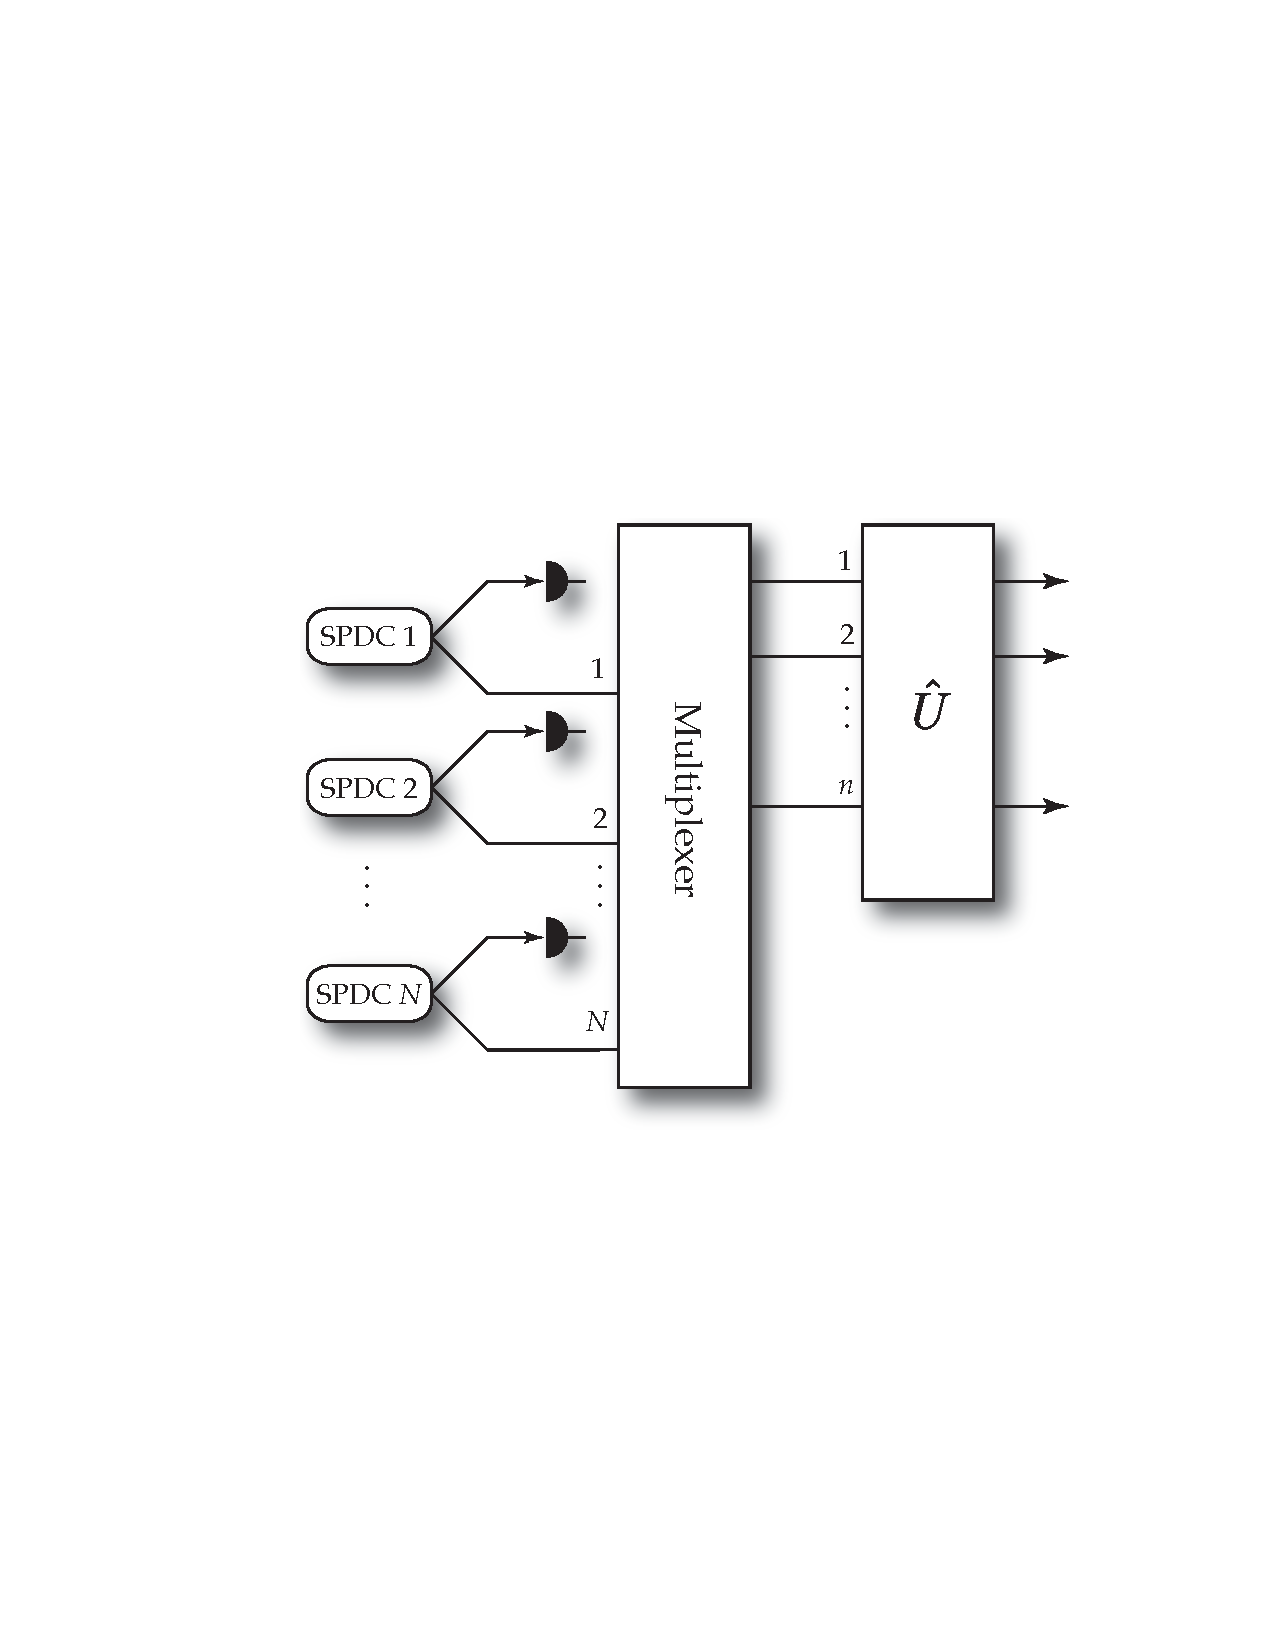
\includegraphics[clip=true, width=0.475\textwidth]{multiplexed_boson_sampling}
\captionspacefig \caption{Model for multiplexed \textsc{BosonSampling}. We operate \mbox{$N\gg n$} SPDC sources in parallel, which are multiplexed to the first $n$ modes of the interferometer $\hat{U}$. With sufficiently large $N$ it becomes asymptotically certain that at least $n$ single-photons will be heralded, thereby successfully preparing the desired \textsc{BosonSampling} input state.} \label{fig:multiplexed_bs}\index{Multiplexed!Boson-sampling}
\end{figure}

Specifically, the probability of at least $n$ successful single-photon heralding events occurring is,
\begin{align}
P_{\geq n} = \sum_{i=n}^\infty \binom{N}{i} 	{P_\mathrm{herald}}^i (1-P_\mathrm{herald})^{N-i},
\end{align}
where,
\begin{align}
	P_\mathrm{herald} = \chi^2(1-\chi^2),
\end{align}
is the probability of a single SPDC source heralding the preparation of a single-photon. This quantity asymptotes to unity for \mbox{$N\gg n$}, as shown in Fig.~\ref{fig:multiplex_bs_res}.

\begin{figure}[!htbp]
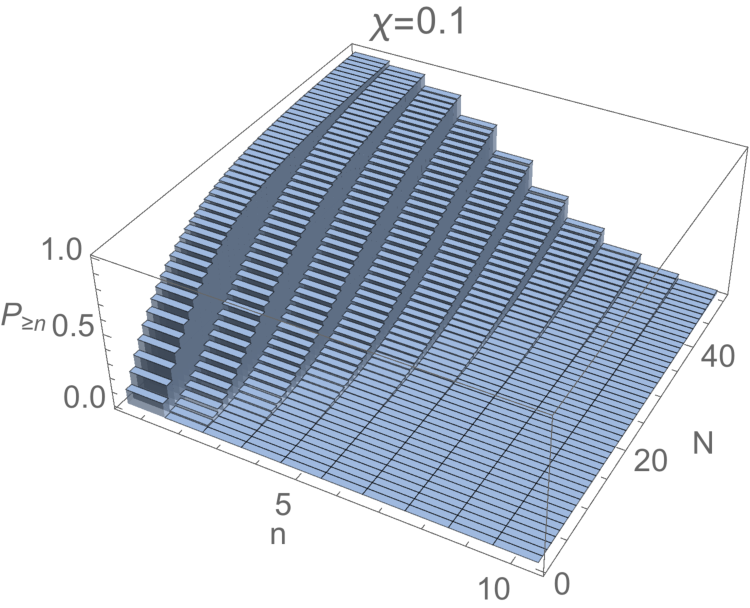
\includegraphics[clip=true, width=0.475\textwidth]{multiplex_bs}
\captionspacefig \caption{Probability of successfully preparing at least $n$ photons for \textsc{BosonSampling} from a multiplexed source comprising a bank of $N$ SPDC sources in parallel. For sufficiently large $N$, we prepare the desired $n$ photons with probability asymptoting to unity.} \label{fig:multiplex_bs_res}\index{Multiplexed!Boson-sampling}
\end{figure}

However, although this procedure works in-principle, it comes at the expense of a large number of sources, $N$, and more challengingly, fast-feedforward. Keep in mind that if we were able to perform complex fast-feedforward, we might be able to do much more (and far more interesting things) than just \textsc{BosonSampling} in the first place!

%
% Scattershot Boson-Sampling
%

\paragraph{Scattershot \textsc{BosonSampling}} \index{Scattershot boson-sampling}

A variation on SPDC-based \textsc{BosonSampling}, known as `scattershot'\index{Scattershot boson-sampling} \textsc{BosonSampling}, has been presented \cite{bib:RandBS}, which obviates the difficultly of fast multiplexing in the approach described previously. Here, rather than inputting an SPDC source into the first $n$ of the $m$ modes, we input a source into \textit{every} mode, i.e $m$ sources in total. We then accept all events with $n$ heralding successes in total, irrespective of the configuration in which they occur. This has the effect of implementing $n$-photon \textsc{BosonSampling} with an additional layer of randomisation on the input modes (i.e a randomisation in the input configuration, $T$, which is ordinarily fixed). However, since the algorithm is already randomised, this additional layer of randomisation does not undermine the complexity proofs, which hold as is. The scattershot model is shown in Fig.~\ref{fig:scattershot_model}.

\begin{figure}[!htbp]
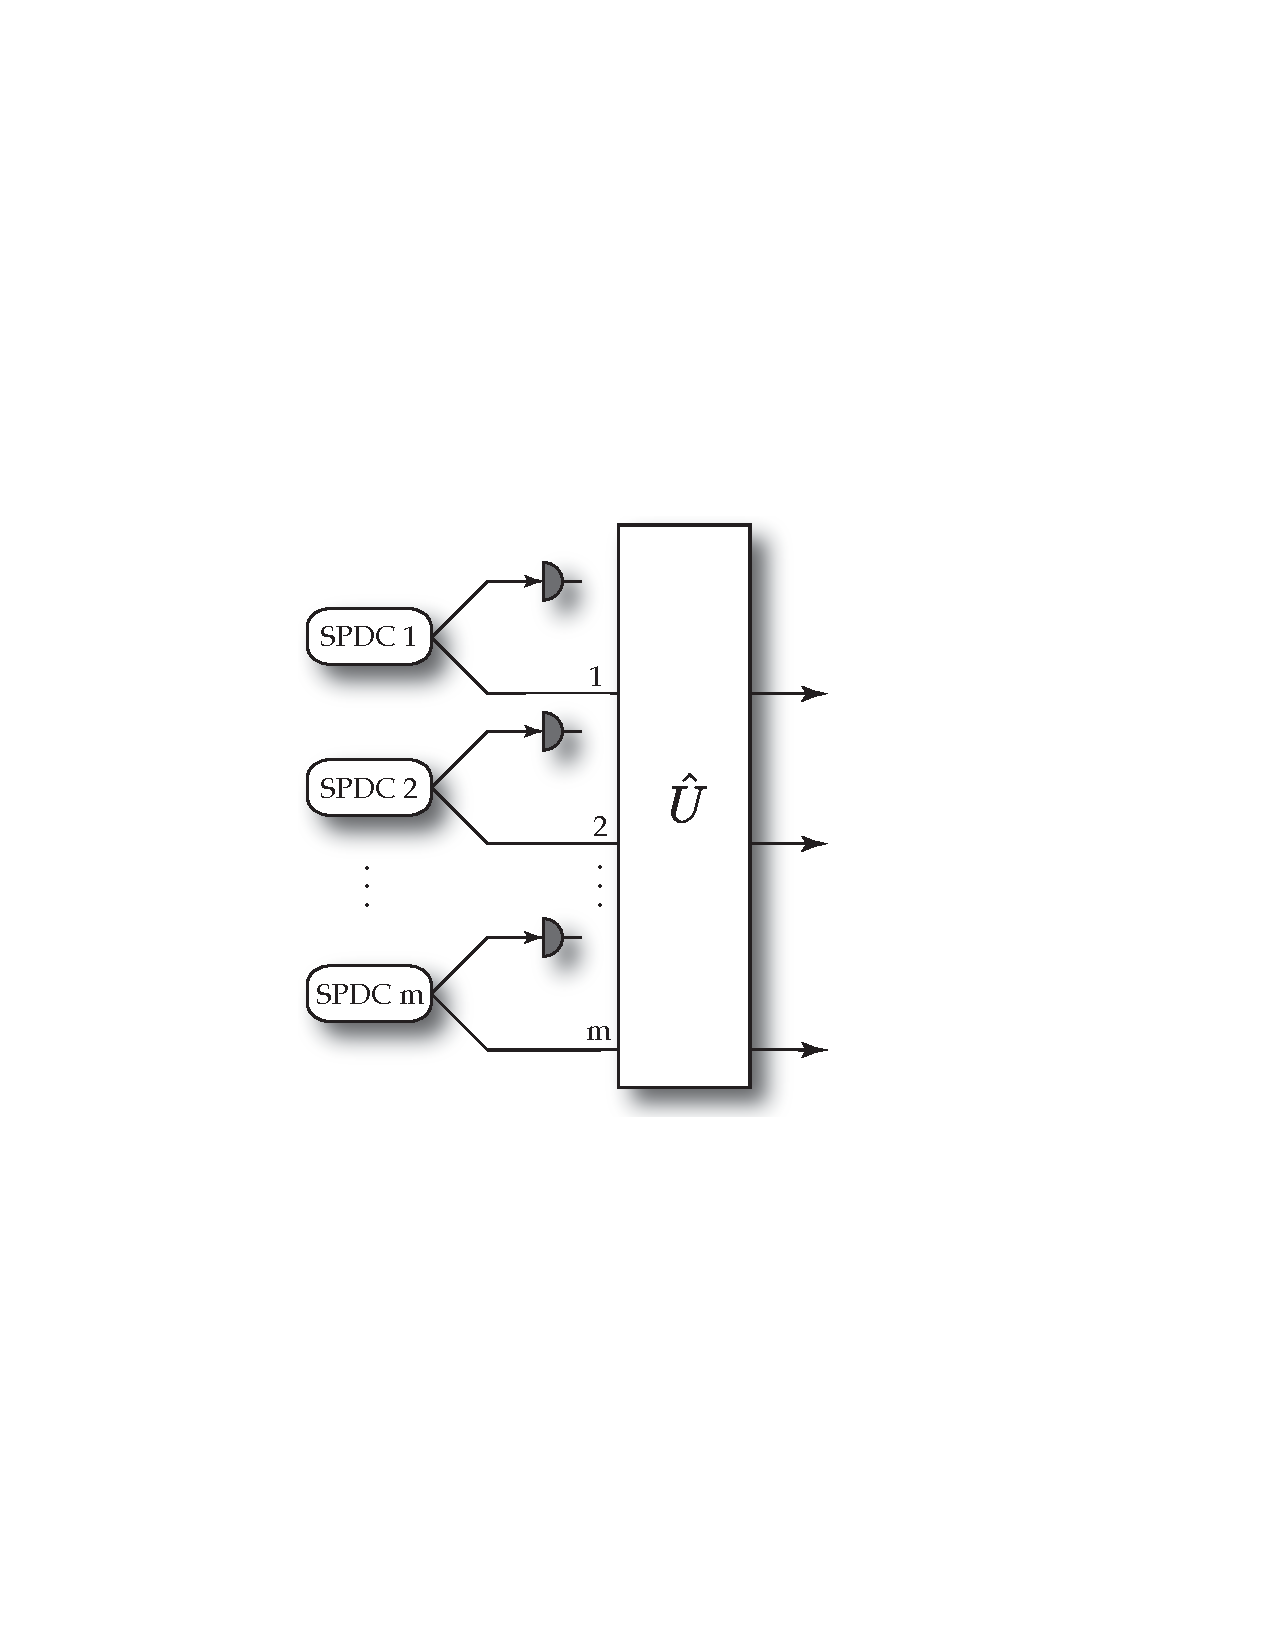
\includegraphics[clip=true, width=0.35\textwidth]{scattershot_model}
\captionspacefig \caption{Model for `scattershot' \textsc{BosonSampling}. An SPDC source is inputted into all $m$ input modes. We post-select upon detecting a total of $n$ photons in the heralding modes, irrespective of their configuration, yielding an $n$-photon instance of \textsc{BosonSampling} with randomised input configuration. Unlike multiplexed architectures, the scheme remains entirely passive, without requiring adaptive fast-feedforward.} \label{fig:scattershot_model}
\end{figure}

By keeping all configurations of $n$ photons, rather than just the \mbox{$\ket{T}=\ket{1}^{\otimes n} \ket{0}^{\otimes (m-n)}$} case, we effectively boost the $n$-photon heralding probability from,
\begin{align}
	P_n = \chi^{2n}(1-\chi^2)^n,	
\end{align}
to,
\begin{align}
	P_n = \binom{n^2}{n}\chi^{2n}(1-\chi^2)^{n^2},	
\end{align}
exhibiting a binomial enhancement in $n$-photon events, yielding a significant improvement in count-rates. For a given desired photon-number $n$, choosing the value for the squeezing parameter, $\chi$, which maximises $P_n$, we obtain the optimised success probability,
\begin{align}
	P_n^{(\mathrm{opt})} \approx \frac{1}{e\sqrt{2\pi(n-1)}},
\end{align}
which exhibits only polynomial scaling against photon-number $n$, and is therefore scalable. This is shown in Fig.~\ref{fig:scattershot_probs}. This is in stark contrast to conventional \textsc{BosonSampling}, where the success probability decays exponentially with photon-number, and is therefore inefficient. Importantly, unlike the multiplexed approach, this efficiency improvement does not require any active elements, remaining in the true spirit of \textsc{BosonSampling}.

\begin{figure}[!htbp]
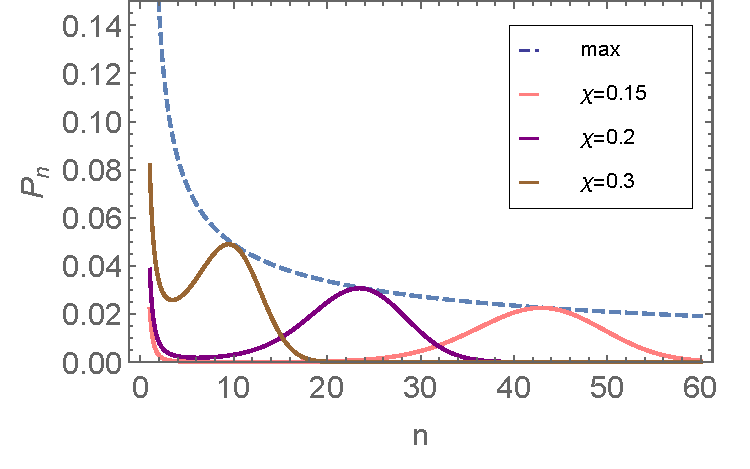
\includegraphics[clip=true, width=0.475\textwidth]{scattershot_probs}
\captionspacefig \caption{Probability of successfully implementing an instance of $n$-photon \textsc{BosonSampling} using the scattershot technique, whereby all input modes are fed with an SPDC source, and all $n$-photon heralding events are accepted, irrespective of their configuration.} \label{fig:scattershot_probs}
\end{figure}

%
% Coherent States
%

\subsubsection{Coherent states} \label{sec:coherent_state_QC} \index{Coherent states!Computation}

A linear optics network acting on a tensor product of coherent state inputs implements simple matrix multiplication\index{Matrix multiplication} on the vector of coherent amplitudes. Specifically, Eq.~(\ref{eq:LO_unitary_map}) implies that for the input multi-mode coherent state,
\begin{align}
\ket{\psi}_\mathrm{in} = \ket{\vec\alpha} = \ket{\alpha_1,\dots,\alpha_m},
\end{align}
where $\alpha_i$ is the coherent amplitude of the $i$th mode, the linear map now takes the form,
\begin{align}
\beta_i = \sum_{j=1}^m U_{i,j} \alpha_j,
\end{align}
where the output state is the separable multi-mode coherent state,
\begin{align}
\ket{\psi}_\mathrm{out} = \ket{\vec\beta} = \ket{\beta_1,\dots,\beta_m}.
\end{align}
Equivalently, this could simply be expressed as the matrix equation,
\begin{align}\label{eq:coherent_state_LO_map}
\vec{\beta} = U\cdot\vec{\alpha}.
\end{align}

Of course this is not strictly a \textit{quantum} computation, since:
\begin{itemize}
\item It can be efficiently classically computed using $O(m^2)$ operations\footnote{Using the na\"ive element-wise approach, which can be further improved upon using more sophisticated contemporary algorithms.}, thus residing in \textbf{P}\index{P}.
\item Coherent states are considered classical states (i.e approximated by laser light\index{Laser light}) with strictly positive Wigner and $P$-functions\index{Wigner function}\index{P-function}.
\item There is no entanglement between modes.
\item The algorithm offers no quantum (exponential) speedup.
\end{itemize}

Despite offering no direct quantum advantage, we introduce this model for restricted computation, since it lends itself very elegantly to a form of homomorphic encryption, to be described in detail in Sec.~\ref{sec:homo_coherent_state}.

The applications for matrix multiplication needn't be stated, as it forms such a ubiquitous elementary primitive throughout linear algebra and in solving systems of differential equations, with applications too many to count.

%
% Other Linear Optics Sampling Problems
%

\subsubsection{Other linear optics sampling problems} \label{sec:other_LO_samp_probs} \index{Linear optics!Sampling problems}

Beyond photonic \textsc{BosonSampling}, much investigation has explored the computational hardness of other types of linear optics sampling problems, using states beyond just single photons.

%
% Hard Problems
%

\paragraph{Hard problems}\index{Hard linear optics sampling problems}

In addition to photonic \textsc{BosonSampling}, several authors have presented strong evidence that other classes of quantum states of light exist, which yield computationally complex sampling problems under the action of linear optics. Most notably, such evidence has been provided for the following:
\begin{itemize}
\item \cite{bib:RandBS} considered two-mode squeezed vacuum (or SPDC) states, a type of Gaussian state with strictly positive Wigner function. This is the same as the scattershot model presented in Sec.~\ref{sec:BS}.\index{Two-mode squeezed vacuum states}\index{Gaussian states}
	\begin{align}
		\ket\psi_\mathrm{in} = \sqrt{1-\chi^2}\sum_{n=0}^\infty \chi^n\ket{n,n}.
	\end{align}
\item \cite{bib:RohdeDisp15} considered photon-added coherent states and displaced single-photon states.\index{Photon-added coherent states}\index{Displaced single-photon states}
	\begin{align}
		\ket\psi_\mathrm{in} &\propto \hat{a}^\dag\ket\alpha,\nonumber\\
		\ket\psi_\mathrm{in} &\propto \hat{D}(\alpha)\ket{1}.
	\end{align}
\item \cite{bib:RohdePhotAdd15} considered photon-added or -subtracted squeezed vacuum states.\index{Photon-added squeezed vacuum states}\index{Photon-subtracted squeezed vacuum states}
	\begin{align}
		\ket\psi_\mathrm{in} &\propto \hat{a}^\dag\hat{S}(\chi)\ket{0},\nonumber\\
		\ket\psi_\mathrm{in} &\propto \hat{a}\hat{S}(\chi)\ket{0}.
	\end{align}
\item \cite{bib:RohdeCat15} considered `cat' states -- superpositions of coherent states.\index{Cat states}
	\begin{align}
		\ket\psi_\mathrm{in} \propto \ket\alpha \pm \ket{-\alpha}.
	\end{align}
\end{itemize}

Preparation of all of these classes of quantum states of light present their own technological challenges, some very daunting, and all much harder to prepare than single-photons. Thus, the ability to outsource their preparation would be a useful application for the quantum cloud.

%
% Easy Problems
%

\paragraph{Easy problems}\label{sec:easy_LO_probs}\index{Easy linear optics sampling problems}

On the other hand, some classes of optical states are known to be efficiently classically simulable under linear optics evolution and photo-detection. This includes coherent states, thermal states, or any state with strictly positive $P$-function\footnote{A strictly positive $P$-function implies that the state can be considered a purely classical mixture of coherent states (each of which are classically efficient to simulate), according to some classical probability distribution.} (Sec.~\ref{sec:exotic}) \cite{bib:SalehQOCCC15, bib:SalehEffSim16}. Furthermore, Gaussian states evolved via linear optics and measured using Gaussian measurements have been shown to be computationally easy to simulate \cite{bib:Bartlett02, bib:Bartlett02b}.

While such negative results might be somewhat depressing, it is extremely insightful to understand these regimes, in the interest of avoiding investing excruciating effort into trying to instead fruitlessly prove that they are hard.

\comment{Cite Saleh/Carlton paper on most optical states generating entanglement. Is it exponential entanglement? If so, is this a necessary but not sufficient condition for computational complexity.}

The simplest example of an easy such problem is coherent state linear optics\index{Coherent states!Linear optics}, as discussed in Sec.~\ref{sec:coherent_state_QC}. Taking this notion further, recall from Sec.~\ref{sec:exotic} that one of the phase-space\index{Phase-space} representations for generic optical states is the $P$-function\index{P-function}, which represents a density operator as a sum over coherent states,
\begin{align}
\hat\rho = \int\!\!\!\int P(\alpha) \ket{\alpha}\bra{\alpha} d^2\alpha.
\end{align}
Here $P(\alpha)$ is a quasi-probability function\index{Quasi-probability functions}. Importantly, iff the $P$-function is strictly non-negative, \mbox{$P(\alpha)\geq 0 \,\,\forall \,\alpha$}, the optical state may be trivially interpreted as a purely classical mixture of coherent states ($P(\alpha)$ would be a delta function for pure coherent states). If, on the other hand, the $P$-function exhibits negativity for any $\alpha$, this interpretation breaks down and is indicative of the state exhibiting non-classical\index{Non-classical states} behaviour.

Alg.~\ref{alg:positive_P_sim} describes an efficient classical algorithm for simulating the output photo-statistics of a linear optics sampler fed with strictly non-negative $P$-function input states \cite{SalehAustinTim}.

\begin{table}[!htbp]
\begin{mdframed}[innertopmargin=3pt, innerbottommargin=3pt, nobreak]
\texttt{
function SimulatePositiveP($\vec{P}$):
\begin{enumerate}
	\item for(m$\in$modes) \{
	\setlength{\itemindent}{0.2in}
	\item Randomly choose a sample $\alpha_m$ from probability distribution function $P_m(\alpha)$\index{Probability distribution function}.
	\setlength{\itemindent}{0in}
		\item \}
		\item Evolve the set of input coherent state samples through the linear optics network,
		\begin{align}
		\vec\beta = U\cdot\vec\alpha.
		\end{align}
	\item for(m$\in$modes) \{
	\setlength{\itemindent}{0.2in}
	\item The probability of measuring $n$ photons in the $m$th mode is given by the distribution,
	\begin{align}
	D_{m,n} &= |\braket{\beta_m|n}|^2 \nonumber \\
	&= e^{-|\beta_m|^2} \frac{{\beta_m}^{2n}}{n!}.
	\end{align}
	\item Choose $n$ from this distribution.
	\setlength{\itemindent}{0in}
	\item \}
	\item return($\vec{n}$).
    \item $\Box$
\end{enumerate}}
\end{mdframed}
\captionspacealg \caption{Efficient classical algorithm for simulating any linear optics sampling problem whose input states have strictly non-negative $P$-functions, with output measured via photon-counting. $\vec{P}$ is the vector of $P$-functions for all modes.} \label{alg:positive_P_sim}
\end{table}

%
% Quantum Walks
%

\subsubsection{Quantum walks} \label{sec:QW} \index{Quantum walks}

Photonic quantum walks (QWs) are the other main contender for implementing restricted quantum computation, without requiring the full spectrum of challenging LOQC operations. The resource requirements are the same as for \textsc{BosonSampling}, the difference being that now instead of choosing a Haar-random unitary matrix for the interferometer, we choose one which encodes a graph. The photons are now referred to as `walkers', and they evolve by following edges within the graph, `hopping' between neighbouring vertices.

With only a single walker (photon), nothing computationally complex can occur in the system, since a single photon evolving under passive linear optics can be efficiently classically simulated\footnote{Note that the literature has described QW schemes, both discrete-time \cite{bib:Lovett10} and continuous-time \cite{bib:Childs09}, that are universal for quantum computation. However, such universal schemes require an exponential number of vertices in the underlying graph, which clearly does not lend itself to efficient optical representation.}. However, once multiple walkers are introduced we have a system with almost identical features to \textsc{BosonSampling}, differing only in the structure of the linear optics unitary.

There are two predominant varieties of quantum walks: discrete- \cite{qwDiscrete:aharanov} and continuous-time \cite{contTimeQW:childs}, which we will now introduce. Algorithms have been described for both the discrete- and continuous-time QW models.

%
% Continuous-Time Quantum Walks
%

\paragraph{Continuous-time quantum walks}\index{Continuous-time quantum walks}

In the continuous-time QW model, a Hamiltonian, $\hat{H}_\mathrm{QW}$, encoding the (Hermitian) adjacency matrix of the QW's graph evolves the walker(s), generating a unitary evolution of the form,
\begin{align}\index{Quantum walks!Hamiltonian}
\hat{U}_\mathrm{QW}(t) = e^{-i\hat{H}_\mathrm{QW}t},
\end{align}
where \mbox{$t\in \mathbb{R}_+$}.

This model lends itself readily to optical wave-guide\index{Waveguides} implementation, where evanescent coupling between neighbouring wave-guides is inherently a continuous-time process. Fig.~\ref{fig:LO_archs}(c) illustrates an example implementation of a linear optics, continuous-time quantum walk on a line in an integrated wave-guide device.

In the context of linear optics, the evolution is best described using the coupled oscillator Hamiltonian\index{Coupled oscillator Hamiltonian},
\begin{align}
	\hat{H}_\mathrm{QW} = \sum_{i,j=1}^m c_{i,j} \hat{a}^\dag_i\hat{a}_j,
\end{align}
where $\hat{a}^\dag_i$ ($\hat{a}_i$) is the photonic creation (annihilation) operator for the $i$th of the $m$ modes, and the Hermitian matrix $c_{i,j}$ encodes the coupling strength between the $i$th and $j$th modes, which could correspond identically to the QW's graph adjacency matrix.

%
% Discrete-Time Quantum Walks
%

\paragraph{Discrete-time quantum walks}\index{Discrete-time quantum walks}

In the discrete-time QW model, each walker has access to an ancillary `coin' Hilbert space, which is used to record the direction of the walker through the graph. At each discrete time-step the coin is used to update the position (vertex) of the walker, before applying a unitary `coin' operator to the coin Hilbert space. The addition of the coin space is necessary to enable such quantum walks to reside on arbitrary graph topologies, whilst retaining unitarity in their evolution. 

We will briefly summarise the discrete-time QW model, as it most readily lends itself to linear optics implementation, and illustrate the parallels with \textsc{BosonSampling}. First, let us consider the standard simple example scenario of a single quantum walker, on a linear graph topology, using a Hadamard coin\index{Hadamard!Gate},
\begin{align}
\hat{C} = \frac{1}{\sqrt{2}}\begin{pmatrix}1 & 1 \\
1 & -1
\end{pmatrix},
\end{align}
which has been experimentally demonstrated using both bulk-optics \cite{bib:Broome10} and time-bin encoding \cite{bib:Schreiber10, bib:RohdeQWExp12}. The walker is defined by two Hilbert spaces: the position $x$, and the coin {$c=\pm 1$}, where $+1$ ($-1$) indicates that the walker is moving to the right (left). The basis states are then $\ket{x,c}$, and the state of the walker takes the form,
\begin{align}
\ket\psi = \sum_{x,c} \lambda_{x,c} \ket{x,c}.
\end{align}
The evolution of the walk is given by the coin and step operators,
\begin{align} \index{Coin operators}\index{Step operators}
\hat{C}\ket{x,\pm 1} &\to \frac{1}{\sqrt{2}}(\ket{x,+1}\pm \ket{x,-1}), \nonumber \\
\hat{S}\ket{x,c} &\to \ket{x+c,c}.
\end{align}
The Hadamard coin operator could be replaced with any arbitrary $\mathrm{SU}(2)$ matrix. The total time-evolution of the walk is then given by,
\begin{align}
\ket{\psi(t)} = (\hat{S}\hat{C})^t\ket{\psi(0)},
\end{align}
where \mbox{$t\in\mathbb{Z}_+$}. Upon measurement, the probability of the walker being at position $x$ is simply given by summing the probabilities over the coins at a given position,
\begin{align}
P(x) = |\lambda_{x,-1}|^2 + |\lambda_{x,+1}|^2.
\end{align}
An example of this kind of quantum walk is shown in Fig.~\ref{fig:QW_ev}.

\begin{figure}[!htbp]
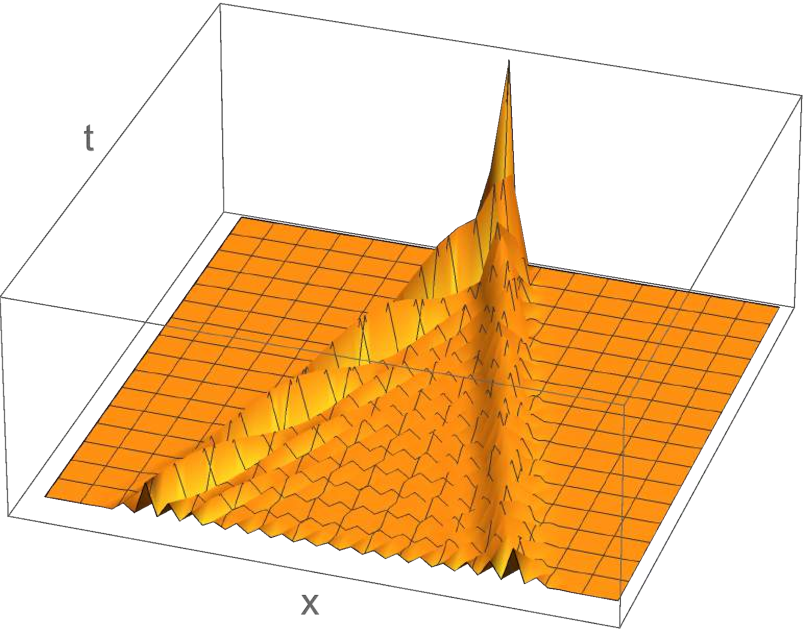
\includegraphics[clip=true, width=0.475\textwidth]{quantum_walk_evolution}
\captionspacefig \caption{Evolution on a 1D quantum walk on a line with a Hadamard coin operator. The walker begins localised at the origin and then spreads out as a superposition over the position space ($x$) with time ($t$). A key feature of this distribution is that its variance grows quadratically with time, compared with linear growth for the equivalent classical random walk. This enhanced spreading forms the basis of the quantum walk search algorithm, with quadratic enhancement compared to a classical search \cite{QWSearch}.} \label{fig:QW_ev}
\end{figure}

The single-walker walk on a linear graph is not of computational interest as it can be efficiently classically simulated. However, the formalism is easily logically generalised to multiple walkers on arbitrary graph topologies. We will illustrate this using the formalism of \cite{bib:RohdeMultiWalk11}, where \textit{walker operators}\index{Walker operators}, rather than walker basis states are evolved under time-evolution (i.e we operate in the Heisenberg picture rather than the Schr{\" o}dinger picture). In an optical context, walker operators are identically photonic creation operators. The walker operators are of the form $\hat{w}(x,c)^\dag$, where $x$ denotes the vertex number currently occupied by the walker, and $c$ denotes the previous vertex occupied by the walker. The single-walker basis states are then of the form $\hat{w}(x,c)^\dag\ket{0}$, where $\ket{0}$ is the vacuum state containing no excitations. Notice the parallels to the previous example of a linear walk, where the coin degree of freedom specifies the direction the walker is following, which effectively acts as memory of the previous position.

The coin and step operators now take the form,
\begin{align}
\hat{C}: \,\,\, &\hat{w}(x,c)^\dag \to \sum_{j\in n_x}A_{c,j}^{(x)} \hat{w}(x,j)^\dag, \nonumber \\
\hat{S}: \,\,\, &\hat{w}(x,j)^\dag \to \hat{w}(j,x)^\dag.
\end{align}
Here $n_x$ denotes the set of vertices neighbouring $x$. The coin operators $A^{(x)}$ are \mbox{$\mathrm{SU}(|n_x|)$} unitary matrices representing the weights of edges within this neighbourhood. The step operator, on the other hand, is simply a permutation. A simple example is shown in Fig.~\ref{fig:QW_arbitrary_graph}.

\begin{figure}[!htbp]
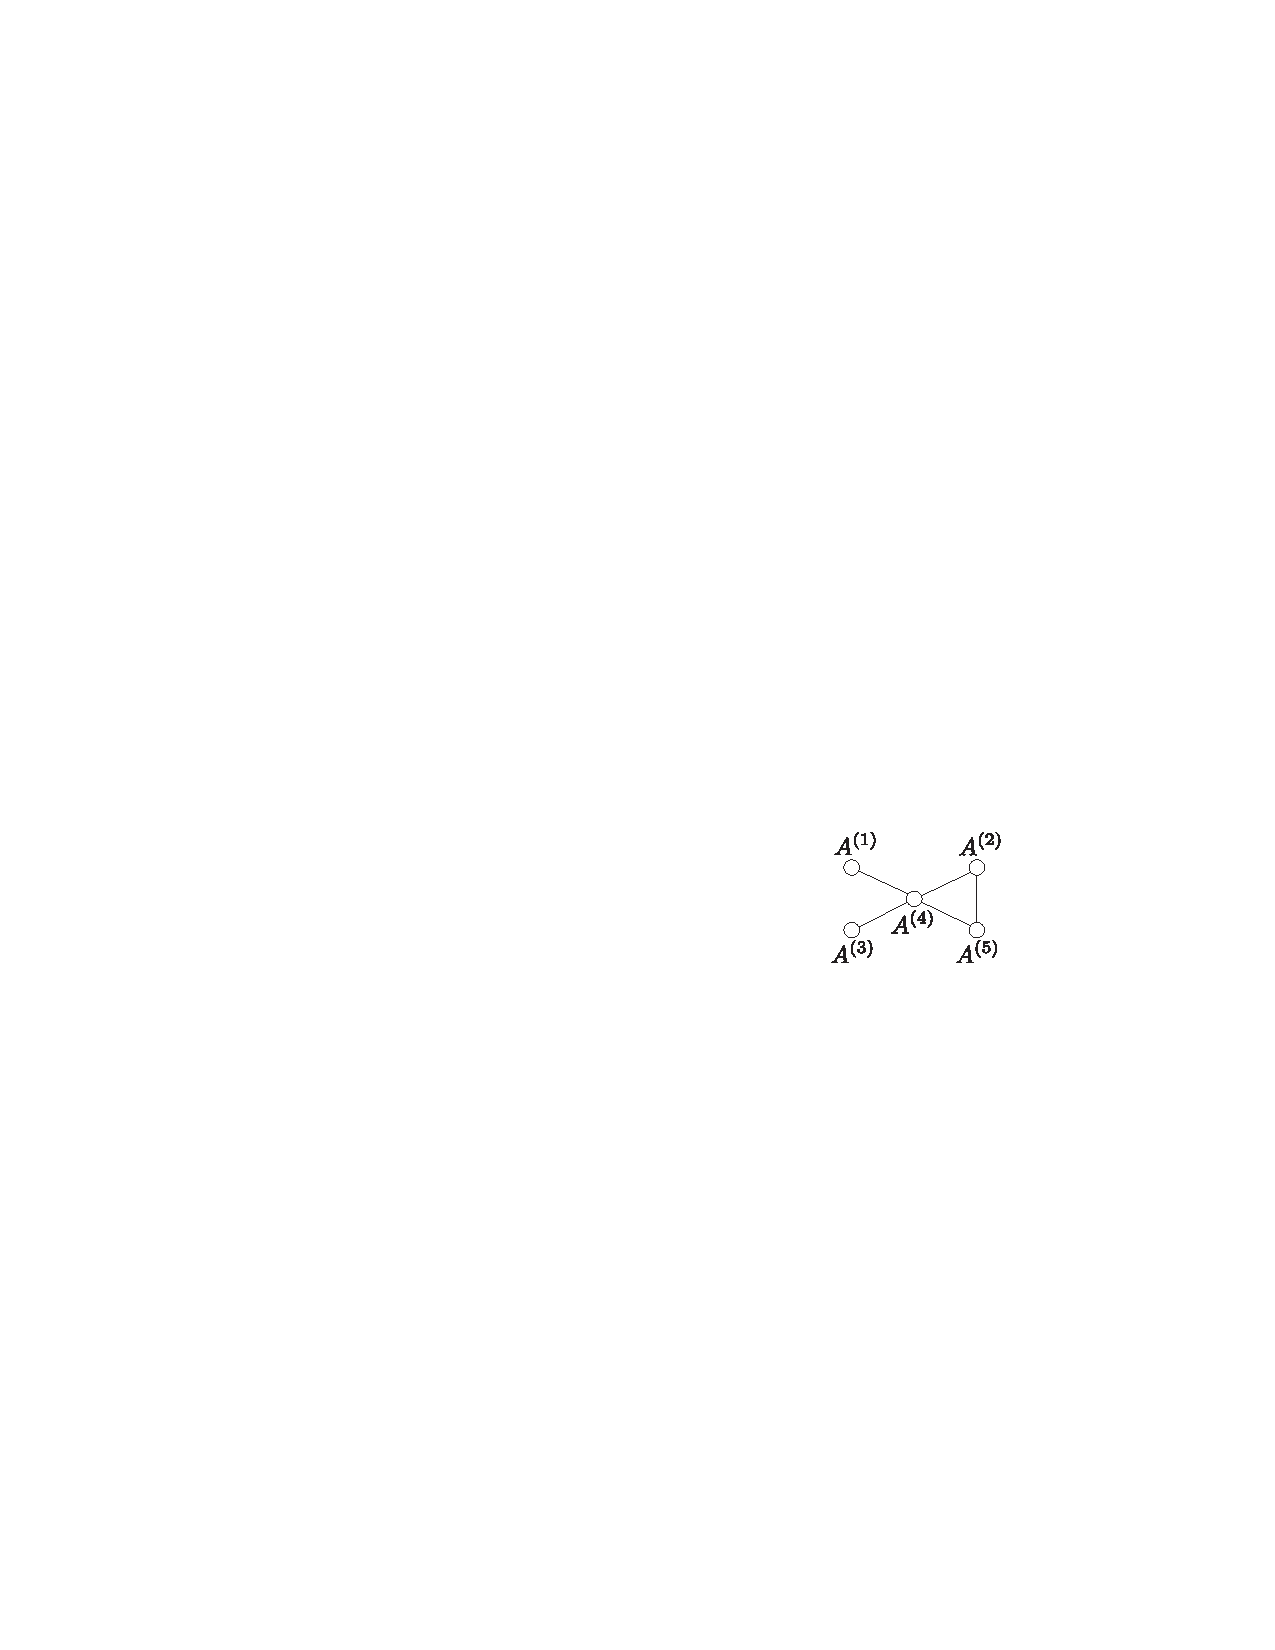
\includegraphics[clip=true, width=0.2\textwidth]{QW_arbitrary_graph}
\captionspacefig \caption{A simple example of a quantum walk on an irregular graph structure. Associated with each vertex $x$ is an $\mathrm{SU}(|n_x|)$ coin operator $A^{(x)}$, where $|n_x|$ is the number of neighbours to $x$.} \label{fig:QW_arbitrary_graph}\index{Quantum walk!Graphs}
\end{figure}

The total time evolution is defined analogously to before,
\begin{align}
\hat{U}_\mathrm{QW}(t) = (\hat{S}\hat{C})^t,
\end{align}
where \mbox{$t\in \mathbb{Z}_+$}.

With this formalism, multiple walkers are easily accommodated for simply with the addition of extra walker operators. Specifically, the $n$-walker basis states are of the form,
\begin{align}
\ket{\vec{x},\vec{c}} \propto \prod_{i=1}^n \hat{w}(x_i,c_i)^\dag \ket{0},
\end{align}
where we have ignored the normalisation factor, which is a function of the number of walkers in each basis state. Any graph topology can be represented, subject to the constraint that all $A^{(x)}$ are unitary. This implies that every vertex must have as many incoming as outgoing edges, which could be either directed or undirected, subject to this constraint.

Now the probabilities of measuring the walkers in different position configurations will be related to matrix permanents, in a similar manner to \textsc{BosonSampling}. But now the permanents will be of matrices that are functions of the set of $A^{(x)}$ matrices characterising the graph, rather than a Haar-random matrix.

It was shown by \cite{bib:RohdeMultiWalk11} that any such walk can be efficiently represented using a linear optics decomposition comprising at most $O(|V|^2)$ optical modes. Such a decomposition for \mbox{$|V|=3$} is shown in Fig.~\ref{fig:QW_LO_representation}.

\begin{figure}[!htbp]
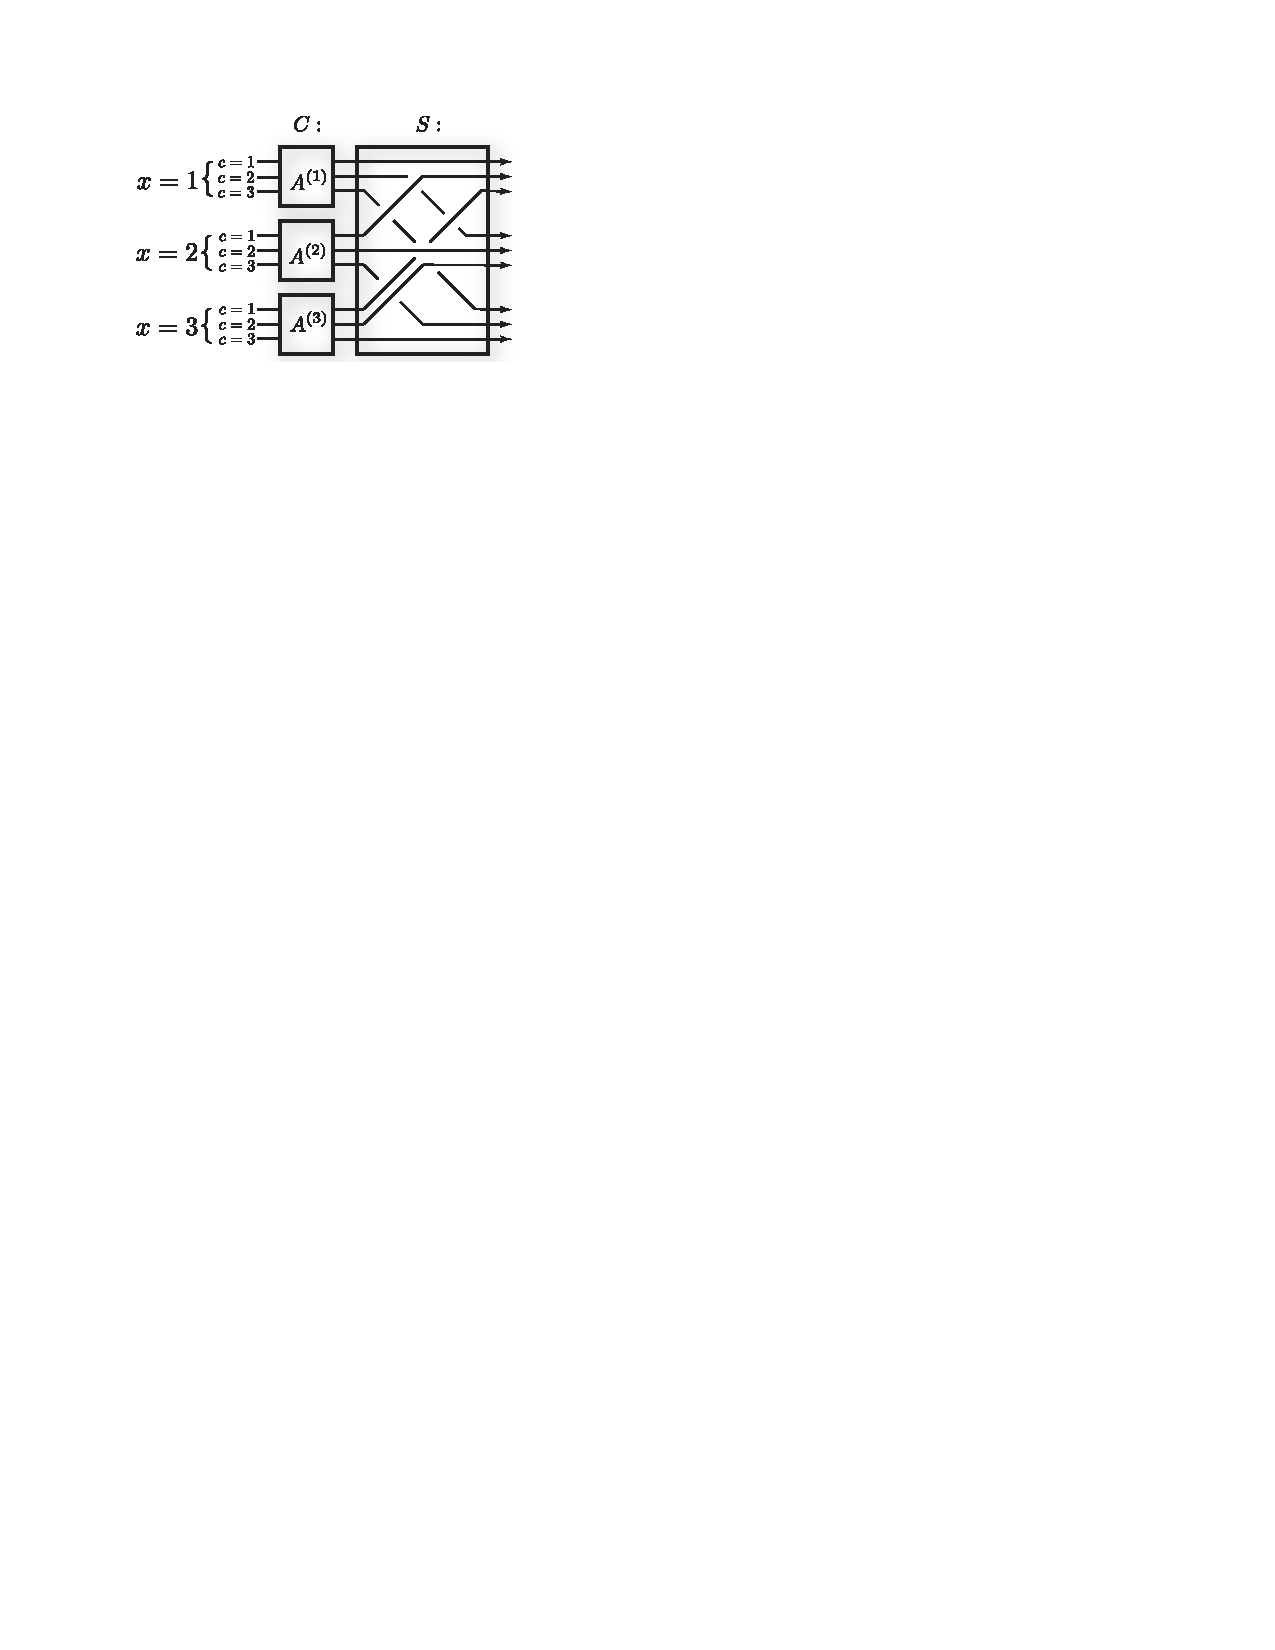
\includegraphics[clip=true, width=0.475\textwidth]{QW_LO_representation}
\captionspacefig \caption{Linear optics decomposition for a single step of an arbitrary 3-vertex discrete-time quantum walk. The coin operators, $A^{(x)}$, may be arbitrary $\mathrm{SU}(3)$ matrices, whereas the step operator is simply a permutation of the optical modes. $O(|V|^2)$ optical modes are required, which scales efficiently.} \label{fig:QW_LO_representation}
\end{figure}

Because of the graph structure of the walk, it lends itself naturally to distributed implementation. We might imagine that different subgraphs -- or `widgets' \cite{bib:Lovett10, bib:Childs09} -- implement different computational primitives or subroutines. These widgets might be proprietary or expensive to implement, and are therefore best outsourced over a network.

%
% Continuous-Variables
%

\subsection{Continuous-variables} \label{sec:CV_QC} \index{Continuous-variables!Quantum computation}

Until now we have focussed on optical systems where quantum information is encoded into discrete variables\index{Discrete-ance variables}, such as photon-number or polarisation. However, quantum states of light can also be considered in terms of continuous-variables (CVs)\index{Continuous-variables} in phase-space\index{Phase-space}.

In this picture, using squeezed states\index{Squeezed states} as a resource, qubits can be closely approximated by vacuum states squeezed in orthogonal directions, where the closeness of the approximation is determined by the squeezing parameter\footnote{In the limit of infinite squeezing the two orthogonally squeezed states becomes orthogonal, enabling the encoding of a genuine qubit.}.

A universal gate set can be constructed, enabling universal quantum computation to be implemented using this encoding. All the necessary elements may be readily implemented using present-day quantum optics technology and numerous CV quantum protocols have been demonstrated \cite{bib:RevModPhys.77.513}. Most notably, very large-scale CV cluster states have been experimentally prepared in the laboratory \cite{nickmenicucci???}.

In the CV picture, instead of representing states using photonic creation operators ($\hat a^\dag$), we express them in terms of the \textit{position} ($\hat x$)\index{Position operator} and \textit{momentum} ($\hat p$)\index{Momentum operator} operators, which can be expressed in terms of creation and annihilation operators as,
\begin{align}
\hat x &=    \sqrt{\frac{\hbar}{2 \omega}}(\hat a + \hat a^\dag), \nonumber \\
\hat p &= -i \sqrt{\frac{\hbar  \omega}{2}}(\hat a - \hat a^\dag), 
\end{align}
where $\omega$ is the optical frequency\index{Optical!Frequency}. These operators obey the commutation relation,
\begin{align}
[\hat x, \hat p] = i \hbar.
\end{align}

The position and momentum operators represent the quadratures\index{Quadratures} of a mode, and correspond to the real and imaginary components of a harmonic oscillator's\index{Harmonic oscillator} amplitude.

The position representation corresponds to expressing a state vector $\ket{\psi}$ in the position basis\index{Position basis representation},
\begin{align}
\ket{\psi} = \int \psi(x)\ket{x}\, dx,
\end{align}
where $\ket{x}$ are the eigenstates of the position operator. Here the wave function in the position representation\index{Position basis representation} is defined as,
\begin{align}
\psi(x) = \braket{x|\psi}.
\end{align}
The state can similarly be expressed in the momentum basis\index{Momentum basis representation},
\begin{align}
	\ket\psi = \int {\tilde\psi}(p) \ket{p}\, dp,
\end{align}
where,
\begin{align}
	{\tilde\psi}(p) = \braket{p|\psi}.
\end{align}

The quadrature eigenstates\index{Quadratures!Eigenstates} are mutually related to each other by a Fourier transform\index{Fourier transform},
\begin{align}
\ket{x} &= \frac{1}{\sqrt{\pi}} \int_{-\infty} ^\infty e^{-2 i x p} \ket{p} \,dp,\nonumber \\
\ket{p} &= \frac{1}{\sqrt{\pi}} \int_{-\infty} ^\infty e^{2 i x p} \ket{x} \,dx.
\end{align}

%
% Encoding Quantum Information Using Squeezed States
%

\subsubsection{Encoding quantum information using squeezed states}\index{Squeezed states!Encoding}

Position and momentum eigenstates are orthogonal and may therefore be employed to encode a single qubit. However, these eigenstates have infinite energy. That is, they are infinitely squeezed in phase-space (Sec.~\ref{sec:squeezed}, \ref{sec:non_lin_opt})\index{Infinite squeezing}. However, position and momentum eigenstates can be closely approximated using finite, but large squeezing. The squeezed states\index{Squeezed states} in the two quadratures will now no longer be orthogonal, but will have overlap that asymptotes to zero as squeezing is increased. Thus, squeezed states can be used to approximate qubits using non-orthogonal basis states. Squeezed states may be prepared directly using a spontaneous parametric down-conversion (SPDC)\index{Spontaneous parametric down-conversion (SPDC)} process (Sec.~\ref{sec:single_phot_src}) \cite{bib:PhysRevLett.75.4337, bib:o2009photonic}. CV encoding using squeezed states is illustrated in phase-space in Fig.~\ref{fig:squeezed_state_encoding}.

\begin{figure}[!htbp]
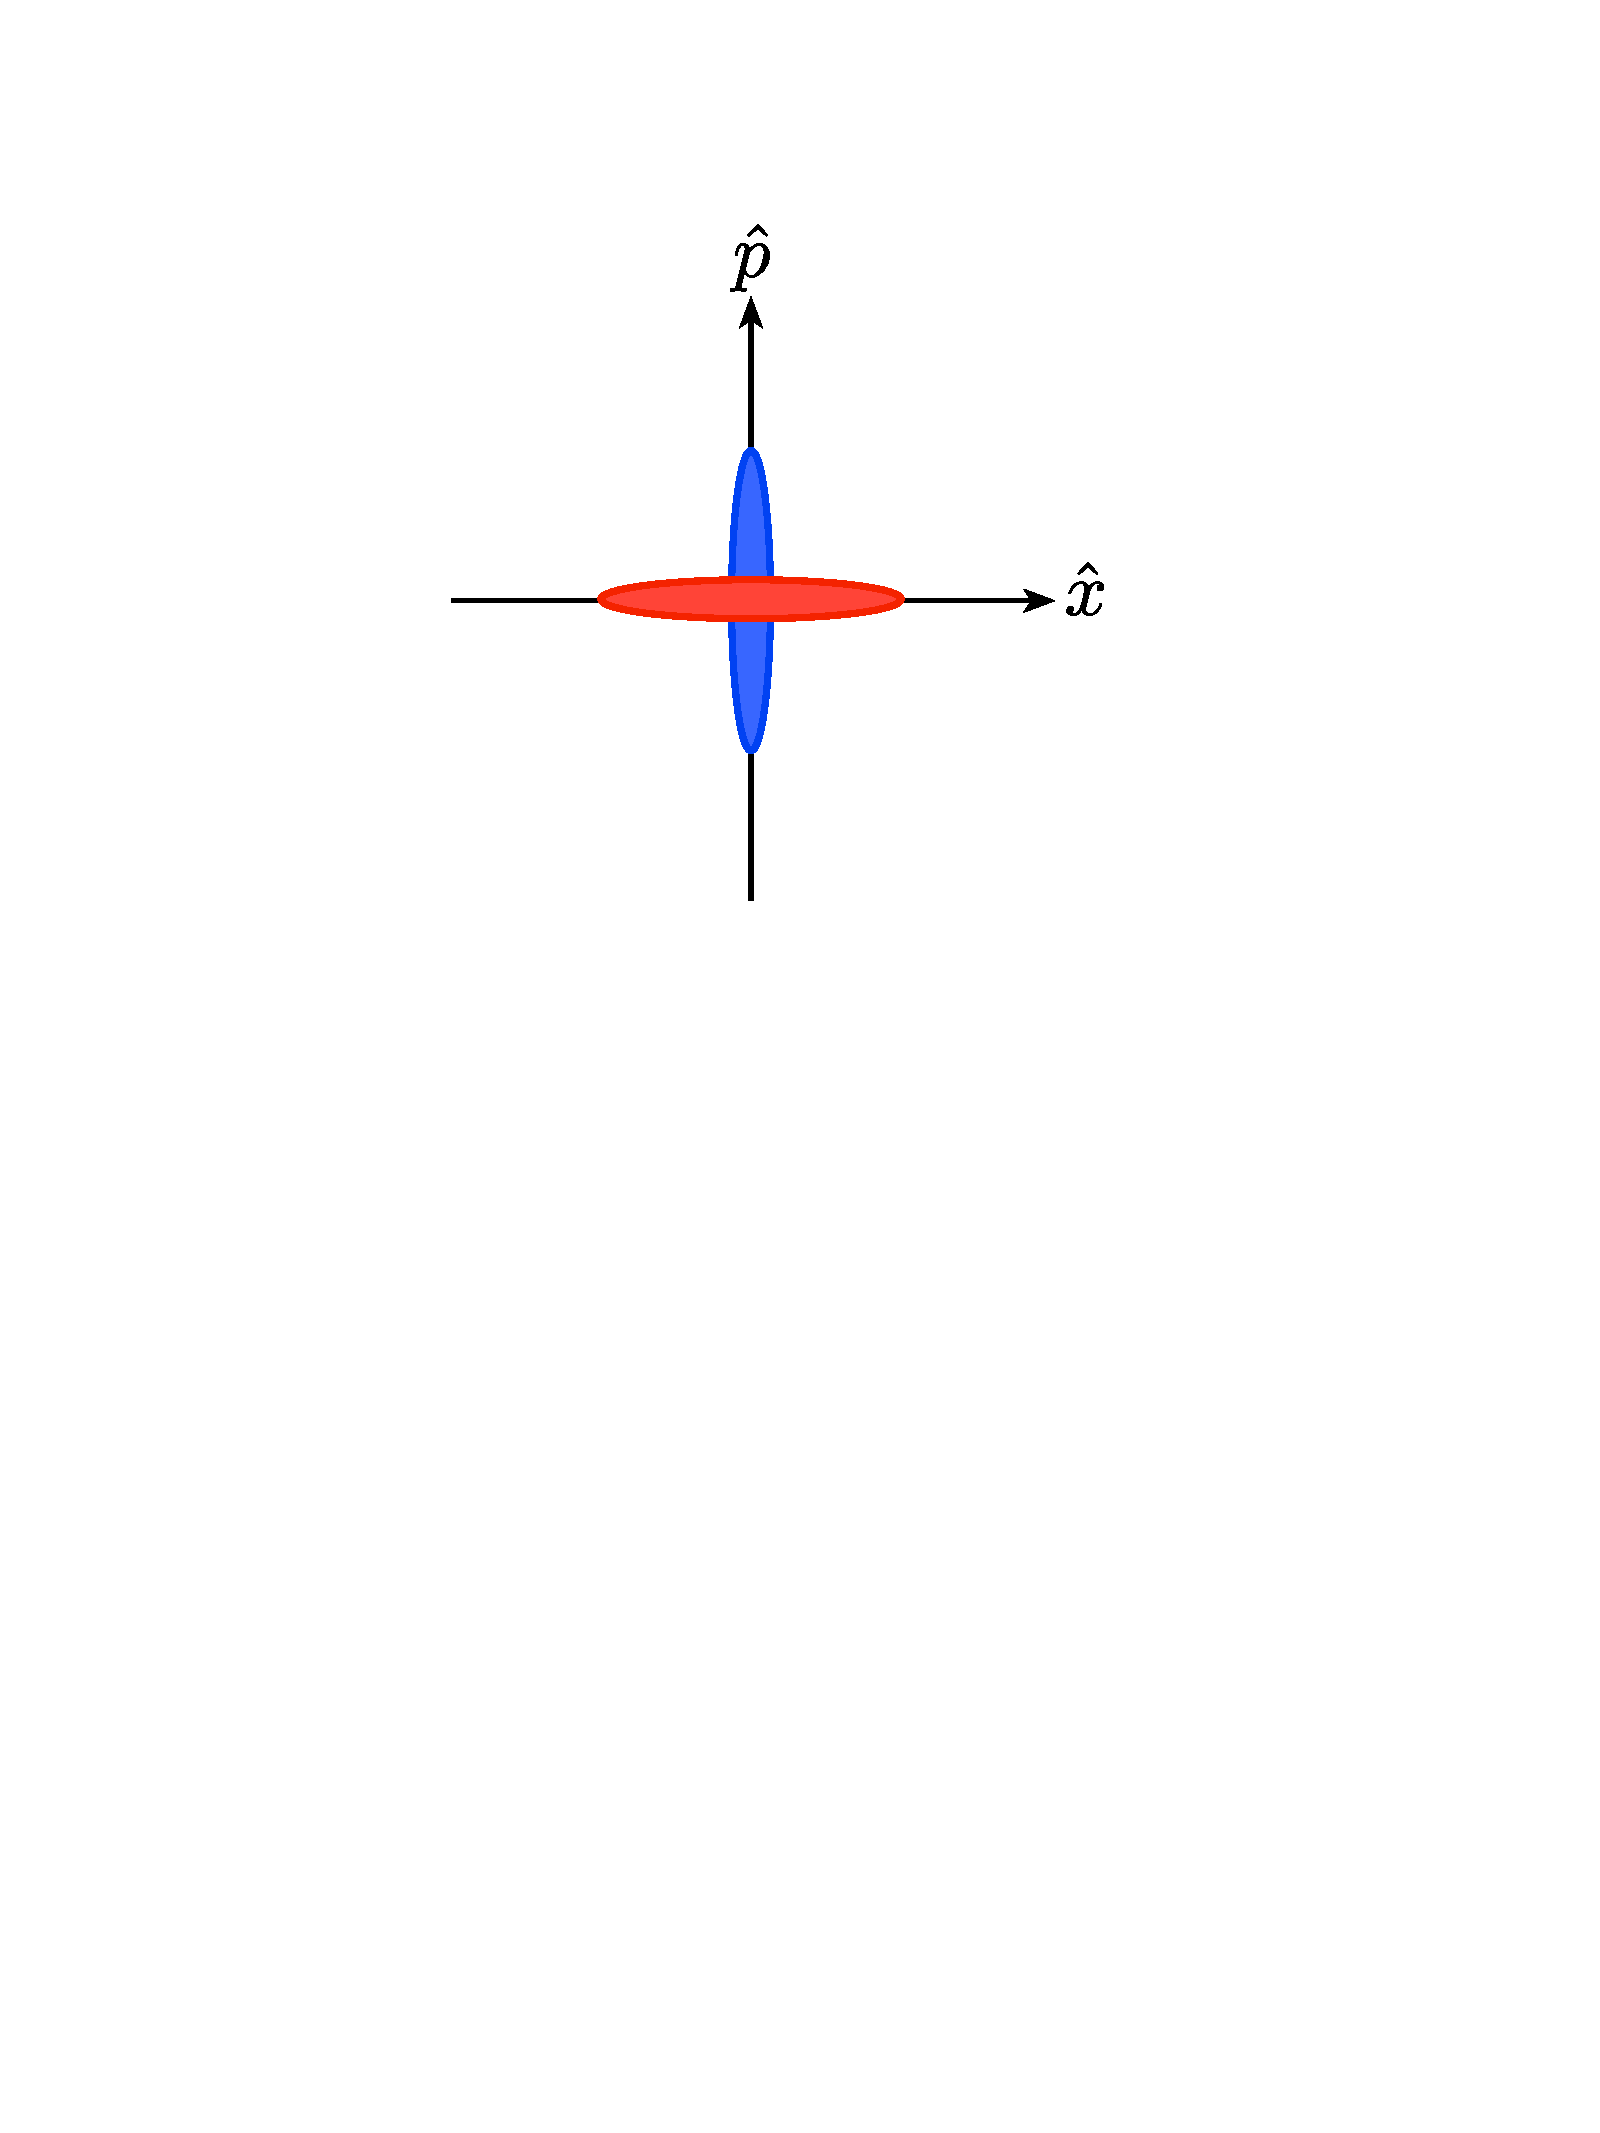
\includegraphics[clip=true, width=0.3\textwidth]{squeezed_state_encoding}
\captionspacefig \caption{Phase-space representation of two squeezed vacuum states, squeezed in the $\hat{x}$ (blue) and $\hat{p}$ (red) directions. In the limit of large squeezing these states become approximately orthogonal and may therefore approximate the encoding of a qubit.} \label{fig:squeezed_state_encoding}	
\end{figure}

Squeezing simply corresponds to a dilation along a particular axis in phase-space. Squeezing is represented using the squeezing operator\index{Squeezing operator},
\begin{align}\label{eq:sq_op}
\hat{S}(\xi) = \exp\left[ \frac{1}{2}(\xi^*\hat{a}^2 - \xi{\hat{a}^{\dag 2}})\right],
\end{align}
where \mbox{$\xi  = r e^{i \varphi}$}, $r$ is known as the squeezing parameter\index{Squeezing parameter}, which will determine the size of the squeezing and \mbox{$\varphi \in [0, 2\pi]$} denotes that axis along which the squeezing is taking place.

\comment{How is squeezing implemented physically in the lab?}

%
% Phase-Shifters
%

\subsubsection{Phase-shifters}\index{Phase-shifters}

A phase-shifter\index{Phase-shifters}, implementing the unitary operation,
\begin{align}
\hat{R}(\theta) = e^{i\theta \hat{n}},
\end{align}
where \mbox{$\hat{n}=\hat a^\dag \hat a$} is the photon-number operator, rotates a state in phase-space by angle $\theta$, implementing the transformation between the position and momentum operators,
\begin{align}
\begin{pmatrix}
\hat x_{\theta}\\
\hat p_{\theta}
\end{pmatrix}
=
\begin{pmatrix}\cos\theta & \sin\theta \\
-\sin\theta & \cos\theta
\end{pmatrix}
\begin{pmatrix}
\hat x\\
\hat p
\end{pmatrix}.
\end{align}
It is evident upon inspection that this can be thought of as a single-qubit rotation in the position/momentum basis. \comment{Is it right that this is a single qubit operation in the x/p basis?}

%
% Bell pairs
%

\subsubsection{Bell pairs}\index{Bell states}\label{sec:CV_bell_pairs}

In the squeezed basis one can prepare Bell pairs in an analogous manner to doing so using single-photon encoding. Namely, mixing two orthogonally squeezed states (squeezed and anti-squeezed states) on a 50:50 beamsplitter generates Bell-type entanglement. This is shown in Fig.~\ref{fig:CV_bell_pair}.

\begin{figure}[!htbp]
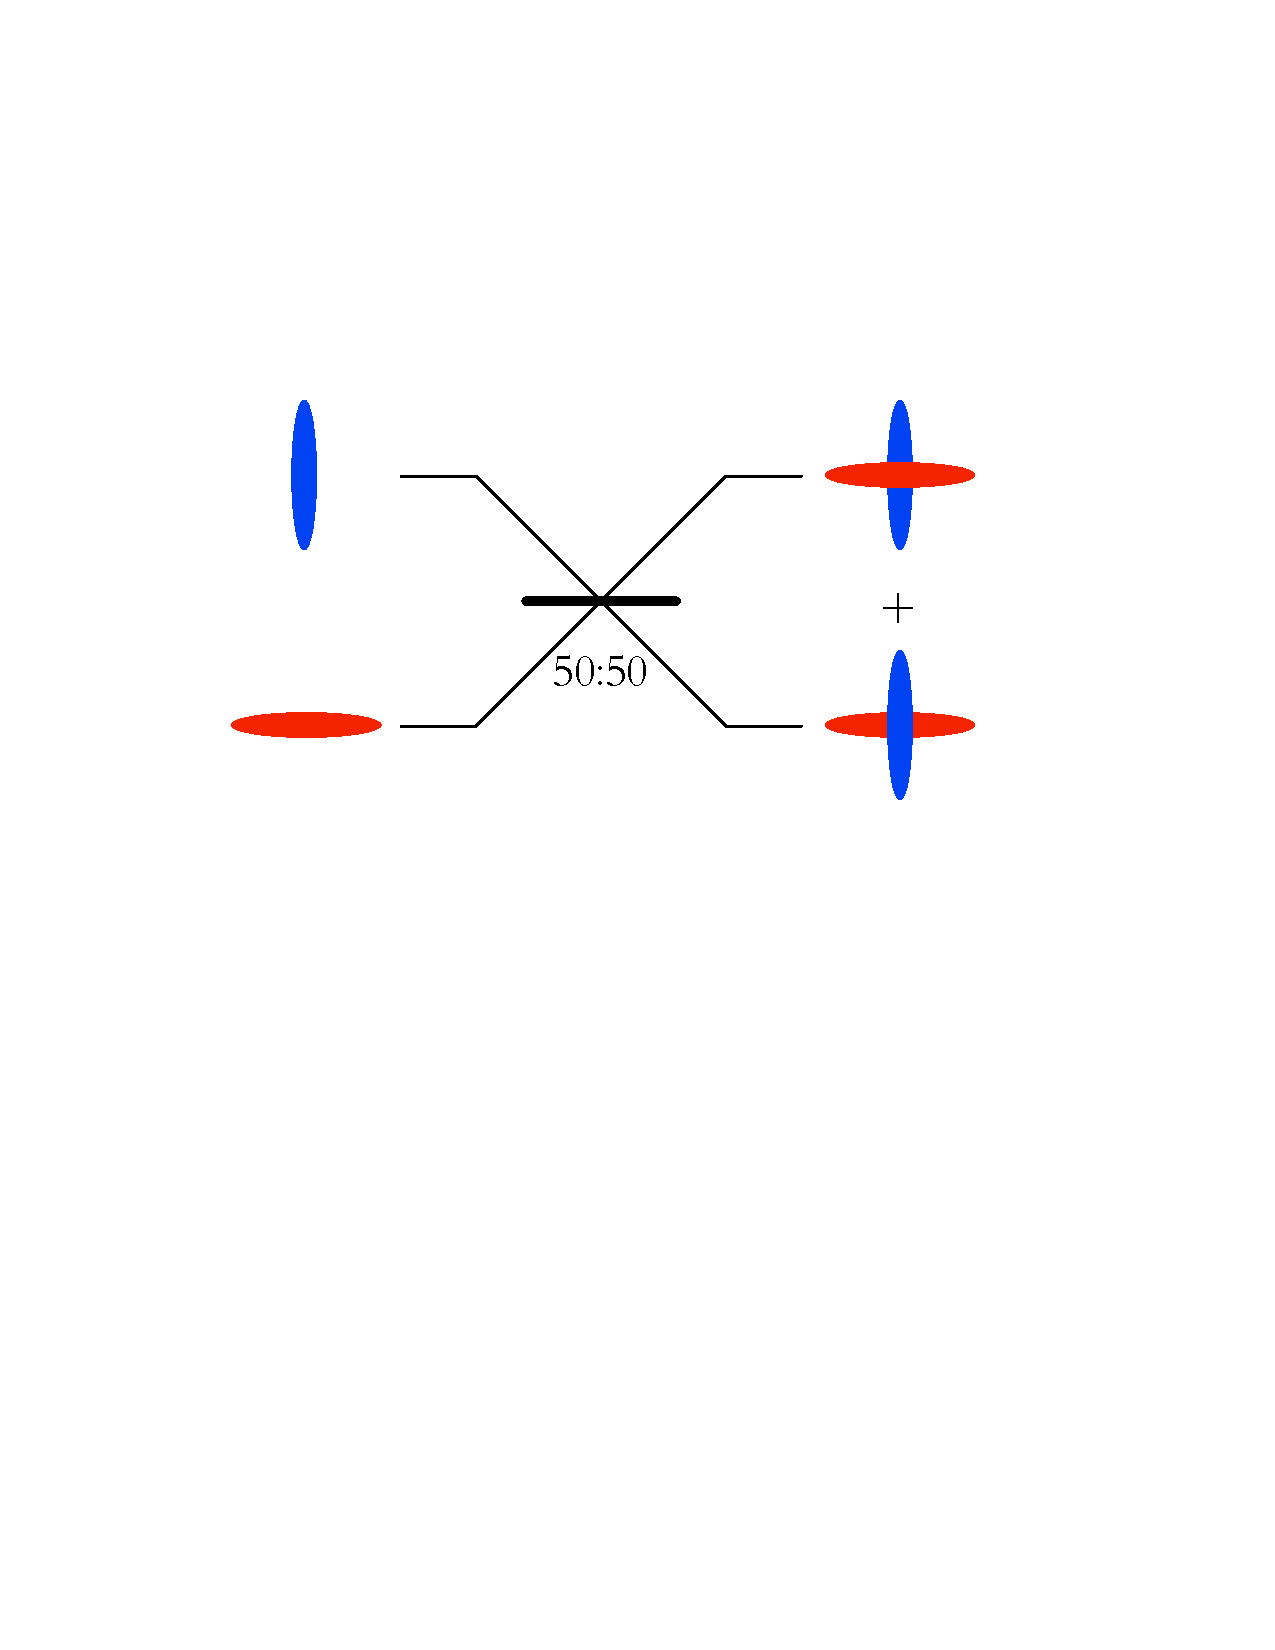
\includegraphics[clip=true, width=0.475\textwidth]{CV_bell_pair}
\captionspacefig \caption{Preparation of a CV Bell pair using a 50:50 beamsplitter to entangled two  squeezed states, squeezed in orthogonal directions in phase-space.}\label{fig:CV_bell_pair}	
\end{figure}

\comment{This is deterministic?}

%
% Measurement
%

\subsubsection{Measurement}

Measurement of CV states may be performed using homodyne detection\index{Homodyne detection} (Sec.~\ref{sec:homodyne}), which perform a projection along an arbitrary axis in phase-space, allowing $\hat{x}$ and $\hat{p}$, or any linear combination of the two, to be directly sampled.

Using a 50:50 beamsplitter to implement the reverse of Bell pair preparation (described previously in Sec.~\ref{sec:CV_bell_pairs}), one can construct a Bell analyser for performing projections in the Bell basis\index{Bell measurements}.

\comment{Is this right?}

\comment{Can we distinguish all 4 Bell states, or just 2 like LOQC?}

%
% Logical Operations
%

\subsubsection{Logical operations}

In the position/momentum picture, the logical generalisations of the Pauli $\hat{X}$ and $\hat{Z}$ qubit gates may be thought of as displacements (Sec.~\ref{sec:non_lin_opt}) in the real and imaginary directions in phase-space \cite{bib:KokLovettBook},
\begin{align}
\hat{X}(s) \equiv \hat{D}(s)	, \, s\in\mathbb{R},\nonumber\\
\hat{Z}(t) \equiv \hat{D}(it), \, t\in\mathbb{R},
\end{align}
where,
\begin{align}\label{eq:disp_op}
\hat{D}(\alpha) = \exp \left[\alpha\hat{a}^\dag - \alpha^*\hat{a}\right],
\end{align}
is the phase-space displacement operator\index{Displacement operator}.

These have the action,
\begin{align}
	\hat{X}(s)\ket{x} &= \ket{x+s},\nonumber \\
	\hat{Z}(t)\ket{p} &= \ket{p+t}. 
\end{align}

The logical generalisation of the CZ gate is,
\begin{align}
\hat{U}_\mathrm{CZ} = e^{\frac{i}{2} \hat x_1 \hat x_2},
\end{align}
which transforms two-mode quadrature eigenstates as,
\begin{align}
\hat{U}_\mathrm{CZ} \ket{s}_1 \ket{t}_2 = e^{\frac{i}{2} s_1 t_2} \ket{s}_1\ket{t}_2.
\end{align}

A full set of circuit model CV gates, universal for CV quantum computing is summarised in Table.~\ref{tab:CV_gates} \cite{bib:RevModPhys.84.621}.

\startnormtable
\begin{table}[!htbp]
\begin{tabular}{ |c|c| } 
 \hline
 Qubit model gate &  CV equivalent \\ 
  \hline\hline
 Pauli $X$ & $\hat{X}(s) = \exp[-i s \hat p]$  \\ 
 Pauli $Z$ & $\hat{Z}(t) = \exp[i t \hat x]$  \\ 
 Phase gate & $\hat{P}(\eta) = \exp[i \eta \hat x^2]$ \\
Hadamard   & $\hat{F}=\exp[i \frac{\pi}{8}(\hat p^2+\hat x^2)]$ \\
CZ		   & $\hat{U}_\mathrm{CZ}= \exp[\frac{i}{2}\hat x_1 \hat x_2]$ \\
CNOT 	   & $\hat{U}_\mathrm{CNOT} = \exp[-2i\hat x_1 \hat p_2]$\\
\hline
\end{tabular}
\captionspacetab \caption{Logical generalisations of a universal gate set to the CV model for quantum computing.\label{tab:CV_gates}}
\end{table}
\startalgtable

\comment{Here explicitly show construction of a CZ gate.}

\comment{Reference to work by Menicucci on fault tolerant implementation of CV QC.}

%
% Cluster States
%

\subsubsection{Cluster states}

\comment{Describe the basic building blocks in a squeezed state cluster state architecture}

\comment{Please add any citations necessary for this entire section. Both theory and experimental work.}

%
% Hybrid Light-Matter Architectures
%

\subsection{Hybrid light-matter architectures} \label{sec:hybrid} \index{Hybrid!Architectures}

It is unlikely that future, large-scale quantum computers will be purely optical. Some other technologies have a more favourable outlook in terms of scalability. Nonetheless, when it comes to networking quantum computers, optics is the natural approach, motivating investigation into hybrid architectures, where qubits are represented using some non-optical system, but entangling operations (EOs)\index{Entangling operations} between them are mediated by optical states and linear optics \cite{bib:Duan06, bib:Beugnon06}.

The natural example is matter qubits which couple to single-photon states, whereupon which-path erasure between coupled optical modes teleports entanglement onto the physical matter qubits\index{Entanglement!Teleportation}.\index{Which-path erasure} Similarly, measurement of the matter qubits may be performed by stimulating the emission\index{Stimulated emission} of photons from them. This idea has been applied to $\lambda$-configuration atomic qubits\index{Atomic qubits}\index{$\lambda$-configuration systems} \cite{bib:BarrettKok05}, shown in Fig.~\ref{fig:barrett_kok}, and atomic ensemble qubits \cite{bib:RohdeAtEns10} (Sec.~\ref{sec:atomic_ens}). The protocol is described in Alg.~\ref{alg:which_path}.

In principle, this technique could be applied to any physical system comprising natural or engineered $\lambda$-configured energy levels, which couple to accessible optical modes. This light-matter coupling\index{Light-matter!Coupling} may require carefully constructed optical cavities\index{Optical!Cavities}, as is the case for single atoms. Alternately, atomic ensemble qubits inherently undergo collective enhancement\index{Collective enhancement} in their light-matter coupling, mitigating the need for optical cavities.

Optically-mediated atomic ensemble architectures are particularly attractive, as discussed in Sec.~\ref{sec:atomic_ens}\index{Atomic ensembles}, owing to their long coherence lifetimes\index{Coherence time}, room temperature operation\index{Room temperature operation}, strong light-matter coupling, and robustness against qubit loss\index{Qubit loss}.

A novel `double heralding'\index{Double heralding} technique, introduced in \cite{bib:BarrettKok05}, allows photon loss\index{Photon loss} to be overcome during which-path erasure. Similarly, quantum states of light can be coupled to two-level quantum systems using Hamiltonians of the form shown in Eq.~(\ref{eq:two_level_hamil}). The preparation of long-distance entanglement between atomic systems has been demonstrated \cite{bib:Matsukevich05, bib:Matsukevich05b}

\begin{figure}[!htbp]
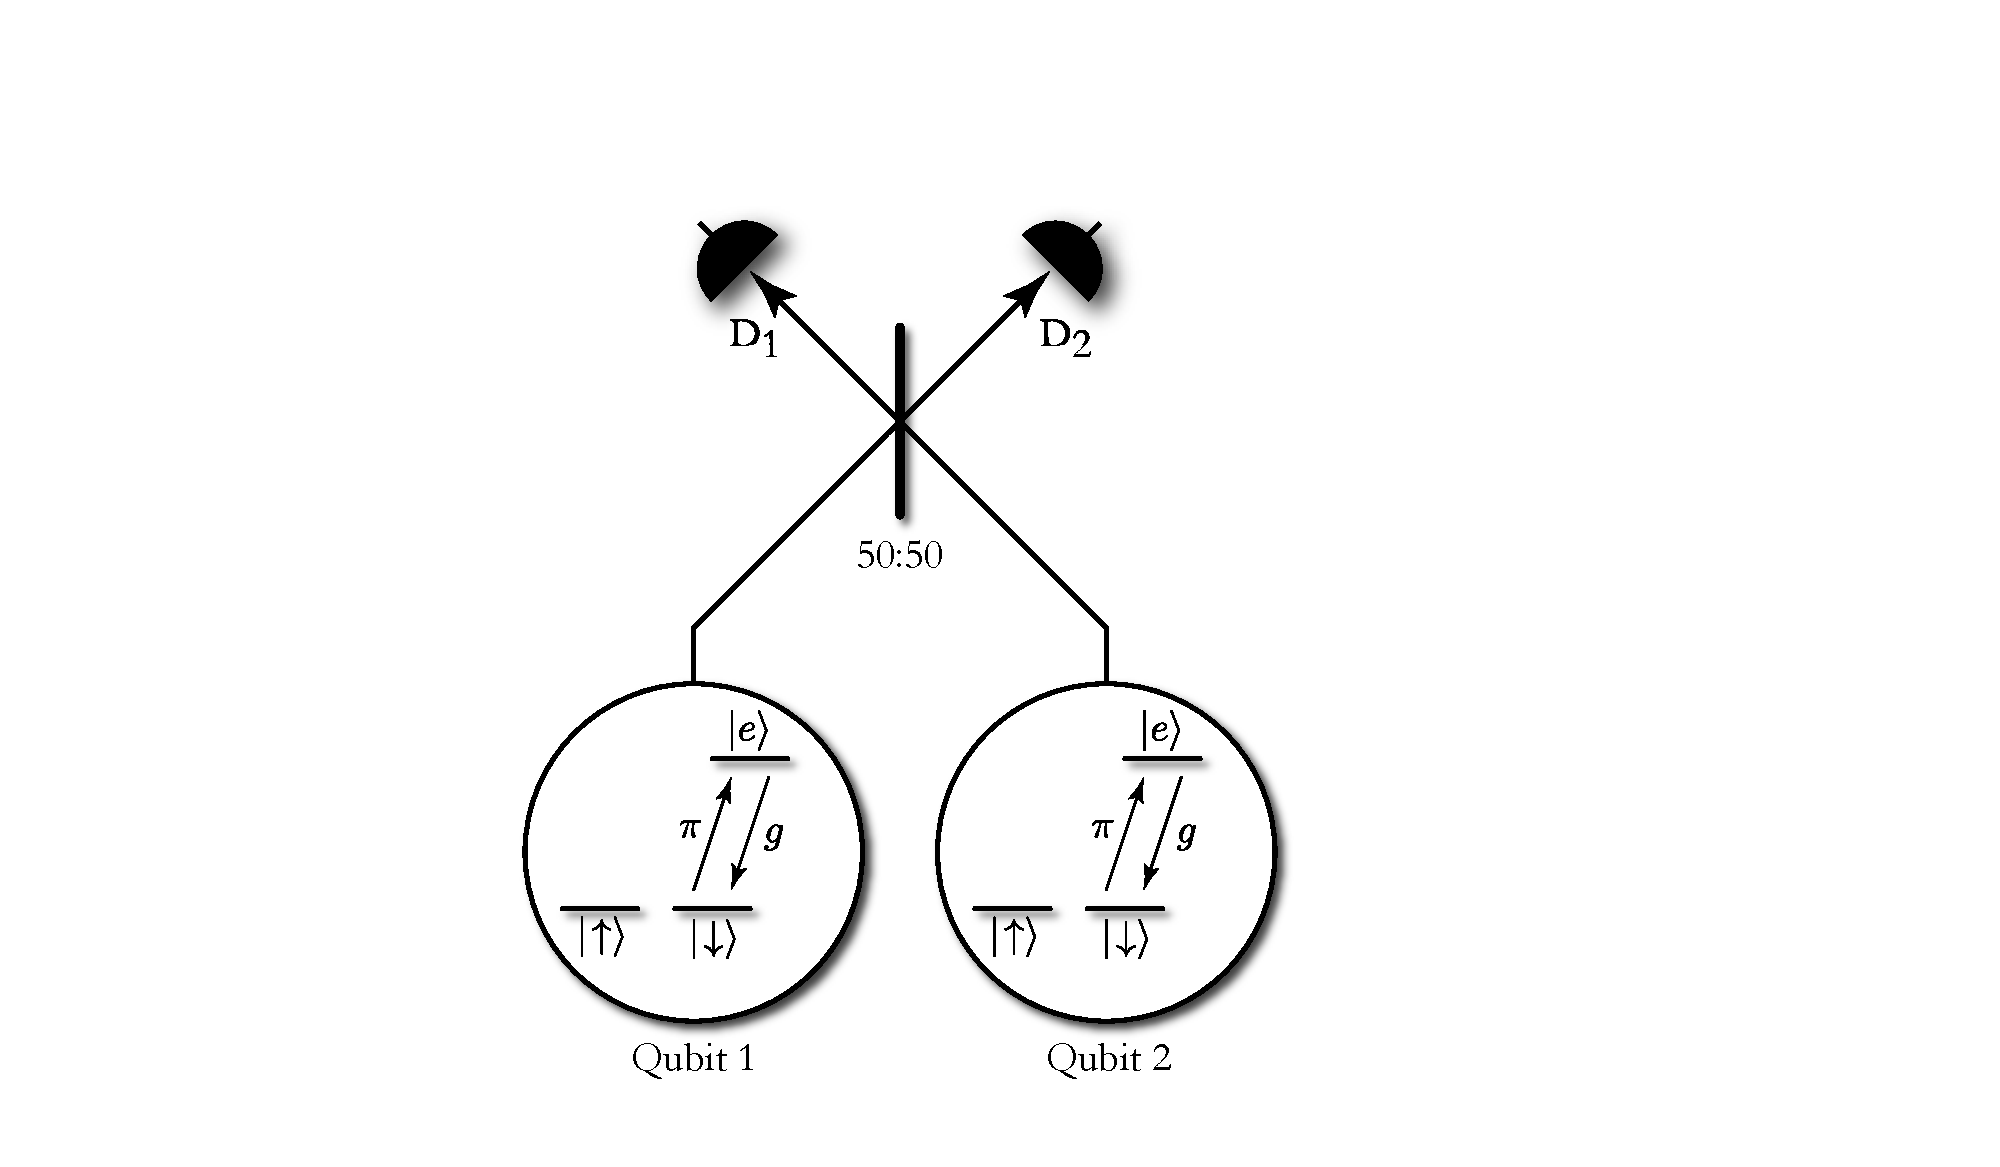
\includegraphics[clip=true, width=0.475\textwidth]{barrett_kok}
\captionspacefig \caption{Two atomic systems in $\lambda$-configurations, each coupled with an optical mode. An EO between them is mediated via linear optics which-path erasure. Each system contains two degenerate ground states, which jointly encode a qubit (\mbox{$\ket{0}\equiv\ket{\!\uparrow}$}, \mbox{$\ket{1}\equiv\ket{\!\downarrow}$}), and an additional excited state ($\ket{e}$), which only couples to the $\ket{\!\downarrow}$ state. A $\pi$-pulse excites the electron from the $\ket{\!\downarrow}$ to the $\ket{e}$ state, after which emission of a photon is associated with a coherent relaxation back to $\ket{\!\downarrow}$. If the two optical modes are interfered on a 50:50 beamsplitter, and a single photon is detected between the two photo-detectors, $D_1$ and $D_2$, the two emission processes become indistinguishable, and which-path erasure entangles the two qubits by projecting them onto a maximally entangled Bell pair. More complicated networks based on this EO allow the preparation of cluster states, enabling universal quantum computation. In a quantum networking context, the matter qubits could be held by a client, and the optical interferometry implementing the computation outsourced to the cloud, i.e the PBS, $D_1$ and $D_2$ are implemented in the cloud. This would also facilitate the preparation of shared entangled states, where different clients possess parts of an entangled state, potentially physically separated over long distances.} \label{fig:barrett_kok}
\end{figure}

The attractive feature of this type of approach is that the actual entanglement is generated using all-optical operations, despite the underlying logical qubits being stationary and potentially physically separated a long distance apart, mitigating the need for direct matter-matter interactions, and enabling distributed computation. Optical interfacing is discussed in Sec.~\ref{sec:opt_inter}. This allows the EOs to be performed remotely in the cloud, without physically moving the stationary qubits. Such hybrid systems present an interesting platform for cloud quantum computing -- despite the qubits being stationary, we are able to outsource the interactions between them to distant servers or even satellites.

Importantly, the beamsplitter mediating the which-path erasure EO is based upon HOM interference, and therefore does not require interferometric stability, making the outsourcing process relatively robust and suitable for long-range operation.

This protocol can be regarded as a variation on the entanglement swapping protocol (Sec.~\ref{sec:swapping}), whereby entanglement between matter qubits and optical modes is swapped onto entanglement between the distinct matter qubits.

Alternately, if there is no direct line of quantum communication between two qubits, an EO can be performed by directly employing the same idea in reverse. We imagine that a third party, such as a satellite, acts as a server for entangled Bell pairs. Two parties receive one qubit each from the pair. Then they perform an EO between their halves of the Bell pair and their local qubits. With appropriate local corrections, mediated by only cheap classical communication, this teleports the action of an EO onto the two qubits, creating a link between them.

Expanding upon this idea, we can envisage distributed models for quantum computation, where the qubits needn't even be of the same physical medium. We could, for example, entangle quantum dot qubits, atomic qubits, and atomic ensemble qubits with one another by coupling them to optical modes and performing which-path erasure between them. This enables distributed quantum computation between hosts possessing quantum infrastructure comprising different physical mediums (provided the photons emitted by those systems may be made indistinguishable, such that HOM interference is possible).

\begin{table}[!htbp]
\begin{mdframed}[innertopmargin=3pt, innerbottommargin=3pt, nobreak]
\texttt{
function WhichPathErasure():
\begin{enumerate}
\item Alice and Bob each prepare an equal superposition of the two logical basis states,
\begin{align}
\ket\psi_\mathrm{in} = &\frac{1}{2}(\ket{\!\uparrow}_{A_1}+\ket{\!\downarrow}_{A_1})\ket{0}_{A_2}\nonumber \\
&\cdot (\ket{\!\uparrow}_{B_1}+\ket{\!\downarrow}_{B_1})\ket{0}_{B_2},
\end{align}
where $A_1/B_1$ denote the matter qubits, and $A_2/B_2$ denote their coupled optical modes.
\item Apply a $\pi$-pulse to each qubit, inducing a \mbox{$\ket{\!\downarrow}\to\ket{e}$} transition,
\begin{align}
\ket\psi_\pi = \hat{U}_\pi\ket\psi_\mathrm{in} = &\frac{1}{2}(\ket{\!\uparrow}_{A_1}+\ket{e}_{A_1})\ket{0}_{A_2}\nonumber \\
&\cdot (\ket{\!\uparrow}_{B_1}+\ket{e}_{B_1})\ket{0}_{B_2}.
\end{align}
\item Wait for a coherent relaxation, inducing the transition \mbox{$\ket{e}\to\ket{\!\downarrow}\hat{a}^\dag$}, which emits a single photon,
\begin{align}
\ket\psi_\mathrm{relax} = \hat{U}_\mathrm{relax}\ket\psi_\pi = &\frac{1}{2}(\ket{\!\uparrow}_{A_1}+\ket{\!\downarrow}_{A_1}\hat{a}^\dag_{A_2})\ket{0}_{A_2}\nonumber \\
&\cdot (\ket{\!\uparrow}_{B_1}+\ket{\!\downarrow}_{B_1}\hat{a}^\dag_{B_2})\ket{0}_{B_2}.
\end{align}
\item Apply a 50:50 beamsplitter between the two optical modes,
\begin{align}
\ket\psi_\mathrm{BS} = \hat{U}_\mathrm{BS} \ket\psi_\mathrm{relax} = &\frac{1}{2}(\ket{\!\uparrow}_{A_1}+\ket{\!\downarrow}_{A_1}[\hat{a}^\dag_{A_2}+\hat{a}^\dag_{B_2}])\nonumber \\
&\cdot (\ket{\!\uparrow}_{B_1}+\ket{\!\downarrow}_{B_1}[\hat{a}^\dag_{A_2}-\hat{a}^\dag_{B_2}])\nonumber \\
&\cdot \ket{0}_{A_2}\ket{0}_{B_2}.
\end{align}
\item Conditional upon detecting exactly one photon between the output optical modes, we obtain,
\begin{align}
\ket\psi_\mathrm{out}^{1,0} = \bra{1,0}_{A_2,B_2} \ket\psi_\mathrm{BS} = \frac{1}{2} (\ket{\!\uparrow,\downarrow}_{A_1,B_1} + \ket{\!\downarrow,\uparrow}_{A_1,B_1}), \nonumber \\
\ket\psi_\mathrm{out}^{0,1} = \bra{0,1}_{A_2,B_2} \ket\psi_\mathrm{BS} = \frac{1}{2} (\ket{\!\uparrow,\downarrow}_{A_1,B_1} - \ket{\!\downarrow,\uparrow}_{A_1,B_1}),
\end{align}
which is a Bell pair between the matter qubits.
    \item $\Box$
\end{enumerate}}
\end{mdframed}
\captionspacealg \caption{Using which-path erasure to entangle two $\lambda$-configuration matter qubits via post-selected linear optics. Note that the two matter qubits could in principle be arbitrarily physically separated. Only the emitted photons need be brought together locally for the implementation of a beamsplitter operation. This lends such entanglement generation protocols to distributed implementation.} \label{alg:which_path}
\end{table}

%
% Atomic Ensembles
%

\subsection{Atomic ensembles}

\comment{To do}

%
% Ion Traps
%

\subsection{Ion traps}\index{Ion traps}

\comment{To do. Talk about optical interfacing.}

%
% Artificial Atoms
%

\subsection{Superconducting circuits}\index{Superconductors!Circuits}\label{sec:artificial_atoms}

Qubits may be engineered by considering the lowest two energy levels of a quantum system. Based on the spacing between their energy levels, such quantum systems are classified into two categories:
\begin{itemize}
	\item Quantum harmonic oscillator type: have equal spacing between energy levels.\index{Quantum harmonic oscillators}
	\item Atomic type: have unequal spacing between energy levels.\index{Artificial atoms}
\end{itemize}
We illustrate these two cases in Fig.~\ref{fig:artificial_atom_energy_levels}, with their corresponding energy level diagrams. The energy levels of these two classes of systems obey,
\begin{align}
E_{n} &= \hbar \omega \left(n+\frac{1}{2}\right) \quad (\mathrm{Oscillator\,levels}), \nonumber \\ 
E_{n} &= -\frac{E_{0}}{n^{2}} \quad (\mathrm{Atomic\,levels}),
\end{align}
where \mbox{$n\in\mathbb{Z}^+$} denotes the discrete energy level, $\omega$ is optical frequency, and $E_0$ is the lowest-lying ground state energy\index{Ground states}.

\begin{figure}[!htbp]
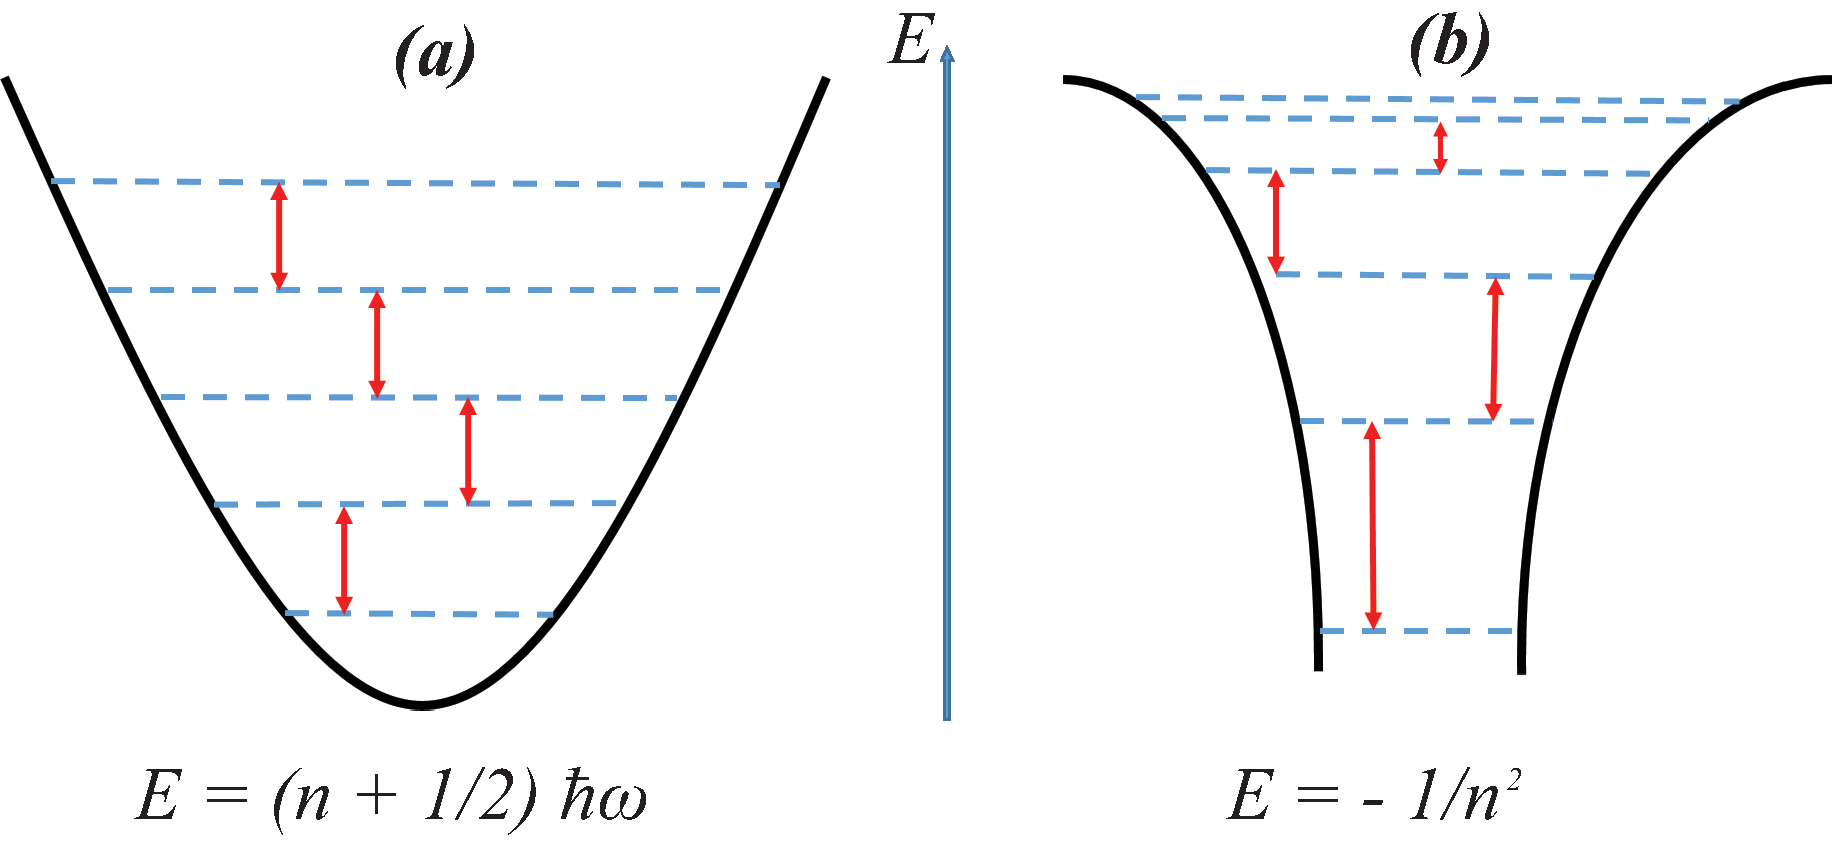
\includegraphics[clip=true, width=0.475\textwidth]{artificial_atom_energy_levels}
\caption{The energy levels of: (a) a quantum oscillator; and, (b) an atomic system. The quantum oscillator exhibits equidistant separation between energy levels, whereas for the atomic system the energy levels are non-uniform.}\label{fig:artificial_atom_energy_levels}\index{Energy levels}
\end{figure}

To construct a qubit we should be able to use external fields\index{Control fields} to control and selectively drive transitions between only two energy levels in the system. Such a procedure is easy to achieve in atomic systems, but it is not possible to address only two levels in a quantum oscillator due to the harmonicity\index{Harmonicity} (equal energy spacing) between energy levels. On the other hand, it's hard to work with individual natural atoms, mainly because of their size, which makes their individual isolation and control very challenging. To overcome this problem, we need to develop new quantum devices with anharmonic\index{Anharmonicity} energy spectra\index{Energy spectra}. Such devices are referred to as \textit{artificial atoms}\index{Artificial atoms}, due to their similarity to natural atoms in the anharmonicity of their energy level spectrum.

One of the most widely used types of artificial atom are superconducting qubits \cite{bib:martinis1985energy, bib:shnirman1997quantum, bib:averin1998adiabatic, bib:devoret2004superconducting, bib:makhlin2001quantum}\index{Superconductors!Qubits}, a class of non-linear quantum circuits\index{Non-linear quantum circuits}. An LC oscillator\index{LC oscillator} composed of an inductor $L$\index{Inductors} and capacitance $C$\index{Capacitors} is a typical example of a linear quantum circuit\index{Linear quantum circuits} with equal spacing. By introducing a Josephson junction\index{Josephson junction} into the linear quantum circuit we can make it non-linear, with anharmonic energy spectrum.

A Josephson junction \cite{bib:josephson1974the} comprises two bulk superconducting materials\index{Superconductors}, separated by a thin layer of insulating material\index{Insulators}. In the superconducting phase the superconductors contain Cooper-pairs\index{Cooper-pairs}, composed of paired electrons. These Cooper-pairs move from one superconducting layer to another through the insulating layer via quantum tunnelling\index{Tunnelling}. The quantum mechanical nature of Josephson junctions is determined by two important energy scales:
\begin{itemize}
\item Josephson coupling energy, $E_{J}$.\index{Josephson coupling energy}
\item Coulomb energy, $E_C$.\index{Coulomb energy}
\end{itemize}
The ratio between these two energy scales determines the energy spectrum of the superconducting qubit. This yields three distinct types of qubits:
\begin{itemize}
\item Voltage-driven charge qubits \cite{bib:bouchiat1998quantum, bib:nakamura1999coherent}.\index{Charge qubits}
	\item Flux-driven flux qubits \cite{bib:friedman2000quantum, bib:van2000quantum}.\index{Flux qubits}
	\item Current-driven phase qubits \cite{bib:martinis2002rabi}.\index{Phase qubits}
\end{itemize} 
These circuits and energy level diagrams for these are illustrated in Fig.~\ref{fig:superconductor_circuits}.

\begin{figure}[!htbp]
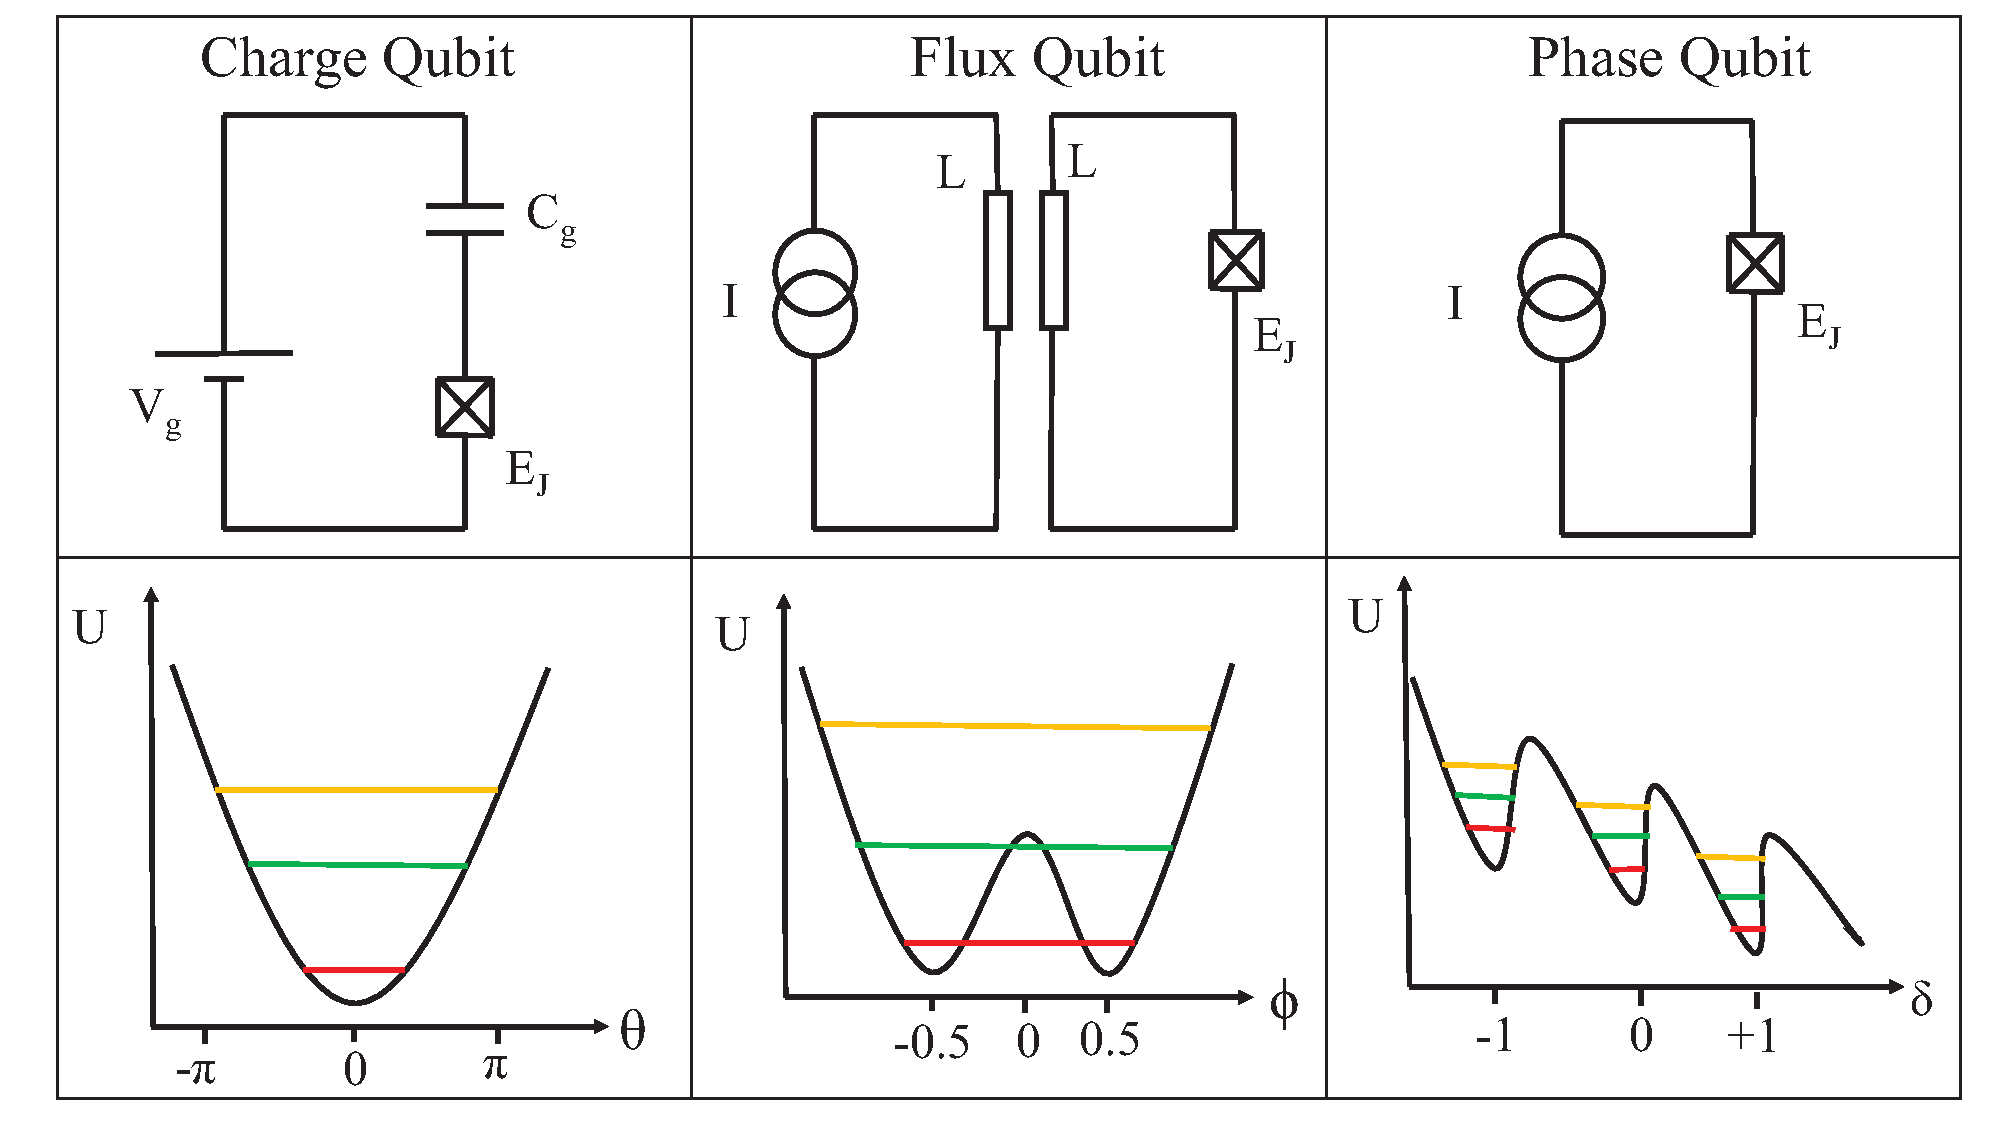
\includegraphics[clip=true, width=0.475\textwidth]{superconducting_qubits}
\caption{Simplified circuits of the different kinds of superconducting qubits, namely the charge qubit, flux qubit and phase qubit. Below each circuit are their respective energy level diagrams.}\label{fig:superconductor_circuits}
\end{figure}

\subsubsection{Charge qubits}\index{Charge qubits}

A non-linear quantum circuit driven by voltage\index{Voltage} is referred to as a charge qubit, whose Hamiltonian takes the form,
\begin{align}
\hat{H} = \frac{\hat{q}^{2}}{2C} - E_{J} \cos \left( \frac{2e}{\hbar} \hat\phi \right).
\label{circuitHamiltonian}
\end{align}
Here $\hat{q}$ is the charge in the superconducting system and $\hat\phi$ is flux\index{Flux}. The total capacitance of the circuit is given by $C$, and $E_{J}$ is the Josephson energy\index{Josephson energy}. The Hamiltonian in Eq.~(\ref{circuitHamiltonian}) can be rewritten as,
\begin{align}\label{eq:charge_qubit_hamiltonian}
\hat{H} = 4E_C (\hat{n} - n_{g})^{2} - E_{J} \cos (\hat{\phi}) .
\end{align}
The variables $\hat{q}$ and $\hat{\phi}$ are canonically conjugate\index{Canonically conjugate} and satisfy the commutation relation,
\begin{align}
[ \hat{\phi},\hat{q} ] = i \hbar.
\end{align}
In a truncated charge basis the Hamiltonian is,
\begin{align}
\hat{H} &= 4 E_C \sum_{n = -N}^{N} (\hat{n} - n_{g})^{2} \ket{n}\bra{n}\nonumber\\
&- E_{J} \sum_{n = -N}^{N-1} \ket{n+1}\bra{n} + \ket{n}\bra{n+1}.
\end{align}

The energy eigenstates are the charge states\index{Charge states} $\ket{n}$, hence these qubits are referred to as charge qubits. In general the charge qubit \cite{bib:bouchiat1998quantum, bib:nakamura1999coherent} is operated in the region,
\begin{align}
	\frac{E_J}{E_C} \approx 1.
\end{align}

Charge qubits are highly sensitive to noise except at particular working points referred to as `sweet spots'\index{Sweet spots}. But it is experimentally difficult to control the voltage and current such that the qubit is maintained at these desired working conditions.

To overcome this, a special design of charge qubit known as the \textit{transmission line shunted plasma oscillation qubit} or `transmon' \cite{bib:koch2007charge}\index{Transmon} with,
\begin{align}
\frac{E_J}{E_C} \gg 1,
\end{align}
was suggested. The transmon is highly robust against external noise compared to the charge qubit. But the energy levels become more and more harmonic\index{Harmonicity} (i.e equally spaced) as we move away from the region,
\begin{align}
	\frac{E_{J}}{E_{C}} \approx 1.
\end{align}
Thus the charge qubits are designed by giving consideration to the trade-off between robustness against external noise and the anharmonicity\index{Anharmonicity} between the levels. A 20-qubit prototype quantum computer developed by IBM\index{IBM} employs transmon-type superconducting qubits \cite{bib:gambetta2017building}. 

\subsubsection{Flux qubits}\index{Flux qubits}

The flux qubit is popularly known as the RF SQUID (Radio Frequency Superconducting QUantum Interference Device)\index{SQUIDs}, which uses an AC current\index{Alternating current}. This qubit can be considered as the magnetic analogue of the charge qubit. In a charge qubit the Josephson junction is driven by a capacitor, but in a flux qubit, a superconducting transformer\index{Superconductors!Transformers} circuit generates the flux which drives the circuit. The Hamiltonian of the circuit is,
\begin{align}
\hat{H} = \frac{\hat{q}^{2}}{2 C_{J}} + \frac{\hat\phi^{2}}{2 L} - E_{J} \cos \left( \frac{2e}{\hbar}(\hat\phi - \phi_\mathrm{ext}) \right).
\end{align}

Here we can observe that there are three energy scales namely,
\begin{align}
E_J,& \nonumber\\
E_{C} &= \frac{2e^{2}}{C},\nonumber\\
E_{L} &= \frac{{\phi_{0}}^{2}}{2L}.
\end{align}
The quantum properties of the qubits depend on the interplay between these parameters. The Cooper-pairs in a flux qubit are confined to a double well potential\index{Double well potential}. The variables $Q$ and the total magnetic flux $\Phi$\index{Magnetic flux} are the conjugate variables, satisfying the commutation relation,
\begin{align}
[\hat{Q},\hat\Phi] = i \hbar.
\end{align}

Flux qubits are very robust against charge noise \cite{bib:you2005fast}, and hence have very long decoherence times\index{Decoherence!Times}, making them one of the most attractive qubit candidates for the construction of quantum computers. The early quantum computing devices developed by D-Wave\index{D-Wave} employ flux qubits \cite{bib:harris2018phase}.

\subsubsection{Phase qubits}\index{Phase qubits}

Current-driven superconducting qubits are referred to as phase qubits \cite{bib:martinis2002rabi}. They are commonly known as DC SQUIDs, and operate in the regime of very high values of $E_{J}/E_{C}$.

The Hamiltonian of a phase qubit is,
\begin{align}
\hat{H} = E_{C} \hat{p}^{2} - I \phi_{0} \hat\delta - I_{0} \phi_{0} \cos \hat\delta,
\label{eq:phase_qubit_hamiltonian}
\end{align}
where $\hat\delta$ is the gauge invariant\index{Gauge invariance} phase-difference operator\index{Phase-difference operator} and the charge on the capacitor is $2pe$. These operators are conjugate variables, satisfying the commutation relation,
\begin{align}
	[\hat\delta, \hat{p}] = i \hbar.
\end{align}

In the phase qubit, Cooper-pairs\index{Cooper-pairs} experience a washboard potential\index{Washboard potential}. Since their decoherence times\index{Decoherence!Times} are very small compared to flux and charge qubits, they are not that widely employed.

\subsubsection{Quantum gates}\index{Quantum gates}

To build useful quantum information processing devices, we require quantum gates to act upon our superconducting qubits. This is a field under active development \cite{bib:blais2004cavity, bib:chow2011simple, bib:chow2013microwave}. Below we provide a brief description of the operation of single- and two-qubit quantum gates based on superconducting qubits.

\paragraph{Single-qubit gates}

A single superconducting qubit, which is coherently controlled using microwaves, can be used as a quantum gate. Let us consider a cavity with resonant frequency $\omega_{r}$\index{Resonant frequency} and drive frequency $\omega_{d}$\index{Drive frequency}, where the difference \mbox{$\Delta_{r} = \omega_{r} - \omega_{d}$} is the detuning\index{Detuning} between the cavity and the drive. When \mbox{$\omega_{d} \approx \omega_{r}$} one can read the state of a superconducting qubit using microwaves. But when \mbox{$\omega_{d} = \omega_{q} \ll \omega_{r}$} the microwave can be used to perform gate operations on the qubit without measuring its state.

A system comprising a superconducting qubit and a microwave can be described using the Jaynes-Cummings Hamiltonian\index{Jaynes-Cummings Hamiltonian},
\begin{align}
\hat{H} = \Delta _{r} \hat{a}^{\dag} \hat{a} - \frac{\Delta_{q}}{2} \hat\sigma_{z} + g (\hat{a}^{\dag} \hat\sigma_{-} + \hat{a} \hat\sigma_{+}) + \xi(t) (\hat{a}^{\dag} + \hat{a}),
\label{eq:driven_jc_hamiltonian}
\end{align}
where $\hat{a}^{\dag}$ ($\hat{a}$) is the creation (annihilation) operator corresponding to the microwave photon, and $\sigma_{+}$ ($\sigma_{-}$) is the spin raising (lowering) operator\index{Spin operators}. The factors \mbox{$\Delta_{r} = \omega_{r} - \omega_{d}$} and \mbox{$\Delta_{q} = \omega_{q} - \omega_{d}$} are the detuning parameters\index{Detuning}. The factor $g$ is the coupling between the microwave photon and the qubit, and $\xi(t)$ is the envelope\index{Envelope} of the microwave pulse. The effective Hamiltonian is,
\begin{align}
\hat{H}_\mathrm{eff} &= \left( \Delta_{r} + \frac{g^{2}}{\Delta} \hat\sigma_{z} \right) \hat{a}^{\dag} a - \frac{1}{2} \left(\Delta_{q} - \frac{g^{2}}{\Delta} \right) \hat\sigma_{z} \nonumber\\
&+ \xi(t) (\hat{a}^{\dag} + \hat{a}) - \frac{g \xi(t)}{\Delta} \hat\sigma_{x}.
\end{align}

To perform an $X$-gate, we choose a drive frequency\index{Drive frequency},
\begin{align}
\omega_{d} = \omega_{q} - \frac{g^{2}}{\Delta}(2 \bar{n} + 1),
\end{align}
which causes the $\sigma_{z}$ term to disappear, leaving us with a pure $\sigma_{x}$ rotation. Using a phase-shifted drive,
\begin{align}
H_{d}(t) = \xi(t) i (\hat{a}^{\dag} - \hat{a}),
\end{align}
one might obtain a pure $\sigma_{y}$ rotation, yielding a $Y$-gate. Finally we note that using a drive,
\begin{align}
	\omega_{d} = \omega_{q} - \frac{g^{2}}{\Delta}(2 \bar{n} + 1) - 2 \xi(t)\frac{g}{\Delta},
\end{align}
we may construct a Hadamard gate. 

\paragraph{Two-qubit gates}

Quantum gates operating on two qubits can be realised in many different ways. But in terms of their construction and operation, they can be divided into two classes. In the first class of quantum gates the superconducting qubits can be tuned over a wide range of frequencies. A good example of this is the iSWAP gate\index{iSWAP gate}, in which two Cooper-pair\index{Cooper-pairs} boxes are coupled via a transmission line resonator\index{Transmission line resonator}. In the rotating frame of reference\index{Rotating frame}, the effective Hamiltonian of the system is,
\begin{align}
\hat{H}_\mathrm{eff} &= \frac{g^{2}}{\Delta} \left( \hat{a}^{\dag} \hat{a} + \frac{1}{2} \right) (\hat\sigma_{z,1} + \hat\sigma_{z,2}) \nonumber\\
&- \frac{g^{2}}{\Delta} (\hat\sigma_{+,1} \hat\sigma_{-,2} + \hat\sigma_{+,2} \hat\sigma_{-,1}).
\end{align}

The parameters of the two qubits can be adjusted by tuning their flux. The interaction between qubits can be turned on and off by tuning the qubits in and out of resonance with one another. The advantage of the first class of quantum gates is that they can be operated in a region where the frequency of the two qubits differ from one another and the interaction between them is very strong. But the disadvantage is that they are sensitive to flux noise, hence requiring extra flux bias lines for tuning them properly.

The second class of quantum gates is built up of superconducting qubits with fixed frequencies, driven by microwaves. The cross-resonance gate\index{Cross-resonance gate}, the bSWAP\index{bSWAP gate} or Bell-Rabi gate\index{Bell-Rabi gate}, and the MAP gate\index{MAP gate} belong to this class. The effective Hamiltonian of the cross-resonance gate is,
\begin{align}
\hat{H}_\mathrm{eff} = - \left( \frac{\tilde{\omega}_{1} - \tilde{\omega}_2}{2} \right) \hat\sigma_{z,1} + \frac{\Omega(t)}{2} \left(\hat\sigma_{x,1} - \frac{J}{\Delta_{12}} \hat\sigma_{z,1} \hat\sigma_{x,2} \right),
\end{align}
where,
\begin{align}
	\tilde{\omega}_{1} &= \omega_{1} + \frac{J^{2}}{\Delta_{12}}, \nonumber\\
		\tilde{\omega}_{2} &= \omega_{2} - \frac{J^{2}}{\Delta_{12}}, \nonumber\\
\Delta &= \omega_{1} -\omega_{2}.		
\end{align}
The factors $\omega_{1}$ and $\omega_{2}$ are the frequencies of the first and second qubits, and $\Delta_{12}$ is the detuning\index{Detuning}. The first qubit is rotating with frequency $\frac{1}{2}(\tilde{\omega_{1}} - \tilde{\omega_{2}})$ around the $Z$-axis, with a little shift in the $X$-direction, yielding an $X$-gate. Similarly we can construct a microwave-activated CZ (MAP) gate\index{MAP gate} using two transmons. The system of two transmons is modelled using a system of two coupled Duffing oscillators\index{Duffing oscillators}. The effective Hamiltonian in the two qubit space reads,
\begin{align}
\hat{H}_\mathrm{eff} &= - \frac{1}{2} \left( \omega_{01} - \frac{\zeta}{2} \right) \hat\sigma_{z,1} - \frac{1}{2} \left( \omega_{10} - \frac{\zeta}{2} \right) \hat\sigma_{z,2} \nonumber\\
&+ \frac{\zeta}{4} \hat\sigma_{z,1} \hat\sigma_{z,2}. 
\end{align}

Through this Hamiltonian we can realise a CZ gate, with gate time $514$ns and high fidelity. The second class of quantum gates have a longer coherence time\index{Coherence time}, since the superconducting qubits can be parked at the sweet spots\index{Sweet spots} of coherence where the effects of noise on the qubits are less substantial. But, control of the qubits is much harder, since we need to maintain them with the same qubit parameters for an extended period of time.

%
% Adiabatic Quantum Computing & Quantum Annealing
%

\subsection{Adiabatic quantum computing \& quantum annealing}\index{Adiabatic quantum computation}\index{Quantum annealing}

\comment{To do. Talk about optical interfacing.}
